\documentclass[11pt,a4paper]{article}
\usepackage{lmodern}
\usepackage{amssymb,amsmath}
\usepackage{ifxetex,ifluatex}
\usepackage{fixltx2e} % provides \textsubscript
\ifnum 0\ifxetex 1\fi\ifluatex 1\fi=0 % if pdftex
  \usepackage[T1]{fontenc}
  \usepackage[utf8]{inputenc}
\else % if luatex or xelatex
  \ifxetex
    \usepackage{mathspec}
  \else
    \usepackage{fontspec}
  \fi
  \defaultfontfeatures{Ligatures=TeX,Scale=MatchLowercase}
\fi
% use upquote if available, for straight quotes in verbatim environments
\IfFileExists{upquote.sty}{\usepackage{upquote}}{}
% use microtype if available
\IfFileExists{microtype.sty}{%
\usepackage{microtype}
\UseMicrotypeSet[protrusion]{basicmath} % disable protrusion for tt fonts
}{}
\usepackage[top=3.3cm,left=3.3cm,right=3.3cm]{geometry}
\usepackage{hyperref}
\hypersetup{unicode=true,
            pdfborder={0 0 0},
            breaklinks=true}
\urlstyle{same}  % don't use monospace font for urls
\usepackage{color}
\usepackage{fancyvrb}
\newcommand{\VerbBar}{|}
\newcommand{\VERB}{\Verb[commandchars=\\\{\}]}
\DefineVerbatimEnvironment{Highlighting}{Verbatim}{commandchars=\\\{\}}
% Add ',fontsize=\small' for more characters per line
\usepackage{framed}
\definecolor{shadecolor}{RGB}{255,255,255}
\newenvironment{Shaded}{\begin{snugshade}}{\end{snugshade}}
\newcommand{\AlertTok}[1]{\textcolor[rgb]{0.94,0.16,0.16}{#1}}
\newcommand{\AnnotationTok}[1]{\textcolor[rgb]{0.56,0.35,0.01}{\textbf{\textit{#1}}}}
\newcommand{\AttributeTok}[1]{\textcolor[rgb]{0.77,0.63,0.00}{#1}}
\newcommand{\BaseNTok}[1]{\textcolor[rgb]{0.00,0.00,0.81}{#1}}
\newcommand{\BuiltInTok}[1]{#1}
\newcommand{\CharTok}[1]{\textcolor[rgb]{0.31,0.60,0.02}{#1}}
\newcommand{\CommentTok}[1]{\textcolor[rgb]{0.56,0.35,0.01}{\textit{#1}}}
\newcommand{\CommentVarTok}[1]{\textcolor[rgb]{0.56,0.35,0.01}{\textbf{\textit{#1}}}}
\newcommand{\ConstantTok}[1]{\textcolor[rgb]{0.00,0.00,0.00}{#1}}
\newcommand{\ControlFlowTok}[1]{\textcolor[rgb]{0.13,0.29,0.53}{\textbf{#1}}}
\newcommand{\DataTypeTok}[1]{\textcolor[rgb]{0.13,0.29,0.53}{#1}}
\newcommand{\DecValTok}[1]{\textcolor[rgb]{0.00,0.00,0.81}{#1}}
\newcommand{\DocumentationTok}[1]{\textcolor[rgb]{0.56,0.35,0.01}{\textbf{\textit{#1}}}}
\newcommand{\ErrorTok}[1]{\textcolor[rgb]{0.64,0.00,0.00}{\textbf{#1}}}
\newcommand{\ExtensionTok}[1]{#1}
\newcommand{\FloatTok}[1]{\textcolor[rgb]{0.00,0.00,0.81}{#1}}
\newcommand{\FunctionTok}[1]{\textcolor[rgb]{0.00,0.00,0.00}{#1}}
\newcommand{\ImportTok}[1]{#1}
\newcommand{\InformationTok}[1]{\textcolor[rgb]{0.56,0.35,0.01}{\textbf{\textit{#1}}}}
\newcommand{\KeywordTok}[1]{\textcolor[rgb]{0.13,0.29,0.53}{\textbf{#1}}}
\newcommand{\NormalTok}[1]{#1}
\newcommand{\OperatorTok}[1]{\textcolor[rgb]{0.81,0.36,0.00}{\textbf{#1}}}
\newcommand{\OtherTok}[1]{\textcolor[rgb]{0.56,0.35,0.01}{#1}}
\newcommand{\PreprocessorTok}[1]{\textcolor[rgb]{0.56,0.35,0.01}{\textit{#1}}}
\newcommand{\RegionMarkerTok}[1]{#1}
\newcommand{\SpecialCharTok}[1]{\textcolor[rgb]{0.00,0.00,0.00}{#1}}
\newcommand{\SpecialStringTok}[1]{\textcolor[rgb]{0.31,0.60,0.02}{#1}}
\newcommand{\StringTok}[1]{\textcolor[rgb]{0.31,0.60,0.02}{#1}}
\newcommand{\VariableTok}[1]{\textcolor[rgb]{0.00,0.00,0.00}{#1}}
\newcommand{\VerbatimStringTok}[1]{\textcolor[rgb]{0.31,0.60,0.02}{#1}}
\newcommand{\WarningTok}[1]{\textcolor[rgb]{0.56,0.35,0.01}{\textbf{\textit{#1}}}}
\usepackage{longtable,booktabs}
\usepackage{graphicx,grffile}
\makeatletter
\def\maxwidth{\ifdim\Gin@nat@width>\linewidth\linewidth\else\Gin@nat@width\fi}
\def\maxheight{\ifdim\Gin@nat@height>\textheight\textheight\else\Gin@nat@height\fi}
\makeatother
% Scale images if necessary, so that they will not overflow the page
% margins by default, and it is still possible to overwrite the defaults
% using explicit options in \includegraphics[width, height, ...]{}
\setkeys{Gin}{width=\maxwidth,height=\maxheight,keepaspectratio}
\IfFileExists{parskip.sty}{%
\usepackage{parskip}
}{% else
\setlength{\parindent}{0pt}
\setlength{\parskip}{6pt plus 2pt minus 1pt}
}
\setlength{\emergencystretch}{3em}  % prevent overfull lines
\providecommand{\tightlist}{%
  \setlength{\itemsep}{0pt}\setlength{\parskip}{0pt}}
\setcounter{secnumdepth}{5}
% Redefines (sub)paragraphs to behave more like sections
\ifx\paragraph\undefined\else
\let\oldparagraph\paragraph
\renewcommand{\paragraph}[1]{\oldparagraph{#1}\mbox{}}
\fi
\ifx\subparagraph\undefined\else
\let\oldsubparagraph\subparagraph
\renewcommand{\subparagraph}[1]{\oldsubparagraph{#1}\mbox{}}
\fi

%%% Use protect on footnotes to avoid problems with footnotes in titles
\let\rmarkdownfootnote\footnote%
\def\footnote{\protect\rmarkdownfootnote}

%%% Change title format to be more compact


\usepackage{titling}

\title{\vspace{3cm}\Huge{Bayesian Inference on Disease Transmission Networks}}
\author{\Large{Stone D. Chen}}

\date
{
    \vspace{5cm}
    \protect\includegraphics[width = 30mm]{uoalogo.png}\\
    \vspace{1.5cm}
    % Change to Masters if applicable
    Bachelor of Science (Honours)\\
    Department of Statistics\\
    The University of Auckland\\
    New Zealand
}

\begin{document}
\begin{titlingpage}
\maketitle
\end{titlingpage}

\pagenumbering{gobble}
\ 
\newpage
\pagenumbering{roman}

\section*{Acknowledgements}
I would like to thank my advisor, Dr. David Welch.
\newpage


\tableofcontents
\newpage



\pagenumbering{arabic}

\begin{abstract}
This dissertation presents an extension of a Bayesian model by for
infectious disease surveillance data by Held et al.
(\protect\hyperlink{ref-held_two-component_2006}{2006}). Their
two-component model captures patterns in a time series of incidence data
with a combination of a Poisson branching process for outbreaks and a
parameter driven component for seasonality. We extend their model to
multiple time series of incidence data that are spatially related, by
incorporating an Erdos-Renyi (ER) random graph. The ER random graph
represents a transmission network between the different spatial regions
and models dependencies between data in those regions. To obtain
parameter estimates, we use the Metropolis-Hastings algorithm and its
variants. We demonstrate estimating the graph parameters on simulated
data.
\end{abstract}

\hypertarget{introduction}{%
\section{Introduction}\label{introduction}}

On the 8th of May 2011, a 42-year-old female presented with
hemolytic-uremic syndrome (HUS), a severe illness that that can lead to
failure of the kidney and the heart. The cause was later identified as
an aggressive strain of \emph{Escherichia coli} known O104:H4. Over the
next two months, O104:H4 caused a severe outbreak of illness throughout
Germany, which at its peak caused 200 new cases per day; the same number
typically seen in an entire year. By July 7th, O104:H4 had affected
3,842 people over 50 of whom later died (\emph{EHEC O104}
\protect\hyperlink{ref-noauthor_ehec_2011}{2011} , pp.~2-3, 11). While
there was initial confusion around the source of the \emph{E. coli}, an
intensive investigation and development of new \emph{ad-hoc} methodology
(Weiser et al. \protect\hyperlink{ref-weiser_trace-back_2013}{2013})
determined the source to be contaminated bean sprouts. This
investigation involved determining the network of connections between
the illness, restaurants, suppliers ,and distributors.

The aim of this dissertation is to develop a statistical method to model
the shipping network of the contaminated sprouts using a graph. The
dataset of interest contains count data from \textasciitilde{} 412
administrative districts in Germany over the time span of the outbreak.
While this work presents a simple Erdos-Renyi random graph, the end goal
is to estimate covariates that affect the probability of transmission
between regions (e.g., the shipping network that transmitted the
\emph{E. coli} contaminated food).

Statistical methods to model infectious disease data typically are
mechanistic models that use expert knowledge of the underyling process
(Pawitan \protect\hyperlink{ref-pawitan_all_2001}{2001}, Ch. 1). One
such model is the Susceptible-Exposed-Infectious-Recovery (SEIR)
(Keeling and Rohani \protect\hyperlink{ref-keeling_modeling_2008}{2008}
, pp.~41-43) model and its variants. In the SEIR model, an entire closed
population of individuals is classified in one of the four eponymous
states. The dynamics of the model works as follows: susceptible
individuals can become exposed when in contact with an infectious
invidual, exposed individuals will eventually become infectious, and
infectious individuals will eventually be recovered and cannot be
re-exposed or infect susceptibles (e.g.~by immunity). If there is data
on what times individuals become susceptible, exposed, infectious, and
removed, parameters surrounding the epidemic of interest can be
estimated. For example, in Groendyke et al.
(\protect\hyperlink{ref-groendyke_bayesian_2011}{2011}), the time spent
in each state is modeled with Gamma random variables and the parameters
of the random variables can be estimated from the time data. Other
parameters of interest such as the intial infected can also be
estimated. They used an extended model to examine the canonical
Haggeloch measles outbreak of 1861 (Groendyke et al.
\protect\hyperlink{ref-groendyke_network-based_2012}{2012}). There they
estimate a contact network between individuals, where covariates can
affect the formation of the contact network and a corresponding
transmission tree. Their network model is a type of exponential random
graph model (ERGM) (Wasserman et al.
\protect\hyperlink{ref-wasserman_social_1994}{1994}). The ERGMs were
designed to be directly analogous to the generalized linear model (GLM).
It allows for statistics surrounding global graph structure such as the
number of triangles and \(k\)-stars to inform the probability of an edge
in a graph. Similar methodology has been applied to other biological
systems (e.g., parasite transmission (White et al.
\protect\hyperlink{ref-white_using_2017}{2017})) as well as social
networks. For example work by Lee et al.
(\protect\hyperlink{ref-lee_network_2018}{2018}) adapted this
methodology to sharing of information on social networks. Here people
are ``infected'' when they see a campaign and subsequently share it.
Their paper also includes a different type of network model, the
preferential attachment model (Albert and Barabasi
\protect\hyperlink{ref-albert_statistical_2002}{2002}). In this model
the probability of adding an edge to a vertex is directly proportional
to the degree of the vertex and creates a ``rich gets richer'' dynamic
and can better describe the degree distribution of social networks.

While effective, this sort of mechanistic model requires data at a
granularity not typical of surveillance data. For example the Hagelloch
measles data contains detailed information on individuals such as the
specific day when different symptoms appear as well as day of death,
when applicable (Albert Pfeilsticker
\protect\hyperlink{ref-albert_pfeilsticker_beitrage_1863}{1863}).
Surveillance data typically does not contain this information and also
often contains other problems such as underreporting (Diggle et al.
\protect\hyperlink{ref-diggle_-line_2003}{2003} , pp.~233-266) which
make it unsuitable to this type of model.

Instead, we begin with a model by Held et al.
(\protect\hyperlink{ref-held_two-component_2006}{2006}) for infectious
disease surveillance data. Held at al.'s method models infectious
disease incidence (i.e., new cases) as a branching Poisson process with
a cyclical endemic parameter. The cyclical endemic parameter models
``seasonality'' (e.g.~seasonal flu patterns) while the Poisson branching
process allows for ``outbreaks'' (e.g.~swine flu, H1N1). Their method
models a single time series of incidence data from a specific location
or region. We extend the model to multiple time series of incidence data
that are spatially related. We incorporate a graph that represents a
transmission network between the different spatial regions (e.g., the
administration district) and allow dependencies between count data in
those regions.

\hypertarget{the-two-component-model}{%
\section{The Two-Component Model}\label{the-two-component-model}}

Held et al. (\protect\hyperlink{ref-held_two-component_2006}{2006})
presents a stochastic model for the statistical analysis of infectious
disease counts that serves as the basis of the extended graph model.

The two components of the model are a simple Poisson branching process
with autoregressive parameter \(\lambda\) and a seasonal component fit
with a Fourier series. These components are described as the
``epidemic'' and ``endemic'' components respectively. Additionally, the
two-component model allows for \(\lambda\) to change over time, which
represents changing infectivity.

A branching process is a stochastic process that is used to model the
evolution (Grimmett and Stirzaker
\protect\hyperlink{ref-grimmett_probability_2004}{2004} , pp.~171-175,
243-255) of population over time. Suppose there's currently one parent
alive (cf., one person infectious). Then in a branching process, this
individual would give birth to a random number of offspring (cf., newly
infected) and then immediately die. Then at the next step, each of those
offspring become parents who individually give birth to a random number
of offspring. If the number of offspring a parent gives birth to comes
from a Poisson distribution with parameter \(\lambda\), then the process
is known as a Poisson branching process. It's in this sense that
\(\lambda\) is an autoregressive parameter since it describes the
relationship between the individuals in the previous time step to the
current one. In this case we assume that the \(\lambda\) value is
constant across individuals and over time (e.g.~\(\lambda\) is some
biological reproduction rate). In the case of the two-component model,
\(\lambda\) is fixed for individuals at a given time, but is allowed to
vary over time. This allows the model to capture the dynamics of disease
outbreaks (Figure \ref{sim_data}).

\hypertarget{two-component-model-notation}{%
\subsection{Two-Component Model
Notation}\label{two-component-model-notation}}

Let \(\vec{Z} = (Z_0, Z_1, ..., Z_n)\) be the count at each time step
\(t\) and let each \(Z_t= Y_t + X_t, t\in \{1,\dots, n\}\). The model is
then specified through \(Z_t | Z_{t-1}\).

\hypertarget{epidemic-component}{%
\subsection{Epidemic Component}\label{epidemic-component}}

The epidemic component is given by
\[Y_t|Z_{t-1} \sim\text{Pois}(\lambda_tZ_{t-1}),\] where \(\lambda_t\)
is the time varing infectivity parameter and \(Z_{t-1}\) is the the
count in the previous time step.

We can think of \(\lambda_t\) as the infectivity of the disease at time
\(t\) with an infected person causing new infections as
\(\text{Pois}(\lambda_t)\). Since each count at time \(Z_{t-1}\)
generates new infected i.i.d \(\text{Pois}(\lambda_t)\), then \(Z_t\) is
the sum of those random variables
\(\sum_1^{Z_{n-1}}\text{Pois}(\lambda_t) =\text{Pois}(\lambda_tZ_{n-1})\).

In this model, the \(\lambda_t\) is allowed to vary over time. We
restrict \(\lambda\) to be piecewise constant with \(K\) change points
at locations \(\theta_1 < \cdots < \theta_K\) with
\(\theta \in \{1,...,n-1\}\). If \(K = 0\) there is no change point and
the \(\lambda\) parameter is constant throughout.

If we only consider the process \(Z_t = Y_t\) (only the epidemic
component), when \(\lambda_t > 1\) an outbreak occurs (Held et al.
\protect\hyperlink{ref-held_two-component_2006}{2006}). When
\(\lambda_t < 1\) then the process ``goes extinct'' or reaches and
remains at 0 with probability 1 (Grimmett and Stirzaker
\protect\hyperlink{ref-grimmett_probability_2004}{2004} , pp.~245). Once
the process reaches a point where \(Z_t = 0\), it remains there as there
are no more infected to create new infected at the next time step.
Allowing \(\lambda_t\) to vary captures many scenarios, for example a
particularly infectious strain of the flu could cause \(\lambda_t\) to
increase above 1 and cause an outbreak. Later, new vaccines and
quarantine procedures can cause the overall infectivity to decrease
below 1.

\hypertarget{endemic-component}{%
\subsection{Endemic Component}\label{endemic-component}}

The endemic component in the model plays two roles: it allows the model
to capture cyclical behaviors in disease (e.g.~seasonal flu) and it also
prevents the branching process from going extinct. The endemic count is
modeled as \[X_t \sim \text{Pois}(\nu_t)\]
\[\log{\nu_t} = \gamma_0 + \sum_{l = 1}^L (\gamma_{2l-1}\sin(\rho l t)+\gamma_{2l}cos(\rho l t)).\]
That is \(\log{\nu_t}\) is fit with a Fourier series. Following Held et
al. (\protect\hyperlink{ref-held_two-component_2006}{2006}), the series
is computed with \(L = 1\) since it was determined higher order
frequencies were insignificant. That is, the truncated series is still
flexible enough to model cyclical patterns seen in disease. The
\(\gamma\)'s are estimated and inform the amplitude of the corresponding
curve. The \(\rho\) term is the base frequency and is set to \(2\pi/52\)
for weekly data.

\begin{figure}
\centering
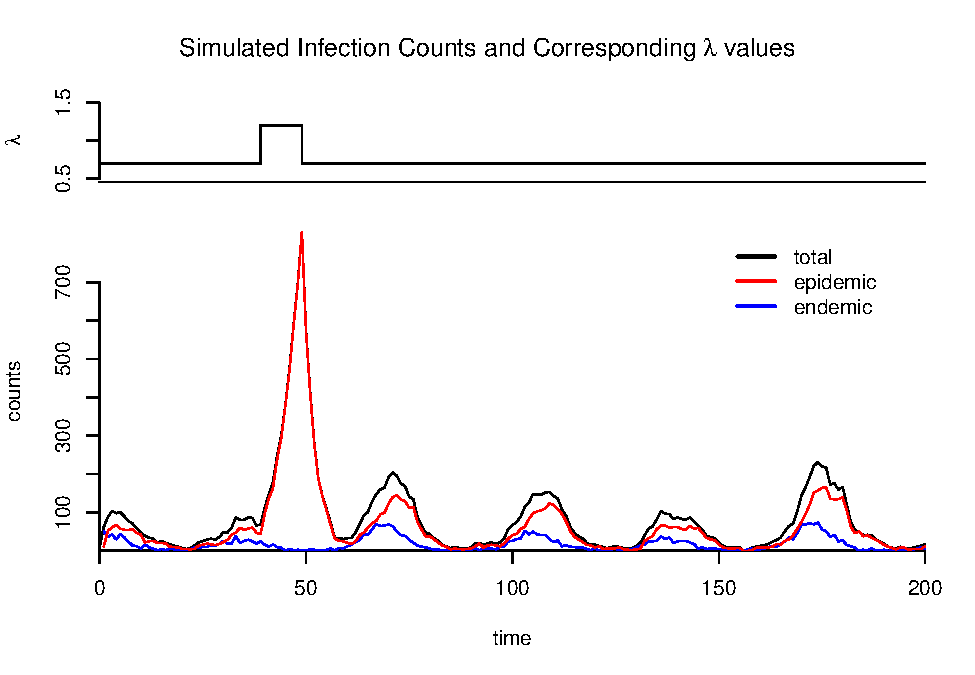
\includegraphics{thesis_draft_files/figure-latex/simulation figure-1.pdf}
\caption{\label{fig:sim_data} A simulated data set. \textbf{Top:}
\(\lambda\) epidemic parameter starts at \(0.7\), increases to \(1.2\)
and then returns to \(0.7\). \textbf{Bottom:} The simulated dataset. Red
shows the count from the epidemic process, blue the endemic and black is
the sum of the two.}
\end{figure}

\hypertarget{likelihood}{%
\subsection{Likelihood}\label{likelihood}}

The probability of the full time series \(\vec{Z}\) given the initial
starting count \(Z_0\) can be factored as a product of the probabilities
of each \(Z_t\) given the previous counts \(Z_{t-1}\),
\[P(\vec{Z}|Z_0,\theta, K, \lambda^{(1)}, \dots, \lambda^{(K+1)}, \gamma_0, \gamma_1, \gamma_2 ) = \prod_{t=1}^b P(Z_t|Z_t{-1}, \theta, K, \lambda^{(1)}, \dots, \lambda^{(K+1)}, \gamma_0, \gamma_1, \gamma_2),\]
where \(Z_t\) is distributed as sum of the Poisson endemic and epidemic
components,
\[Z_t|Z_{t-1}, \theta, K, \lambda^{(1)}, \dots, \lambda^{(K+1)}, \gamma_0, \gamma_1, \gamma_2 \ \ \sim\ \text{Pois}(\nu_t + \lambda_tZ_{t-1}),\]
where the endemic component \(\nu_t\) is described as,
\[\log{\nu_t} = \gamma_0 +  \gamma_{1}\sin(\rho  t)+\gamma_{2}\cos(\rho  t),\]

with \(rho = 2\pi/52\). Lastly, \(\lambda_t\) is piecewise function
described by
\[ \lambda_t =  \begin{cases} \lambda^{(1)}, & t < \theta_0 \\
\lambda^{(k)}, & \theta_{k} \leq t < \theta_{(k-1)} \\
\lambda^{(K+1)}, & t \geq \theta_K \end{cases}.\]

\hypertarget{multiple-locations-connected-by-a-graph}{%
\section{Multiple locations connected by a
graph}\label{multiple-locations-connected-by-a-graph}}

We would like to extend our data from a univariate time series of counts
\(Z_t\) to multiple time series of counts \(Z_{i,t}\) where \(i\) now
indexes separate time series. In this case we will say the \(i\) indexes
individual ``cities'' so \(Z_i\) represents the disease counts in city
\(i\). Now, a city \(i\)'s epidemic disease count at time \(t\) is
modeled as a function of both its own disease count \(Z_{i,t-1}\) and
possibly other cites' counts as well.

This dependence between cities is represented by a graph \(G\) where
\(N_v\), the number of vertices in graph is fixed and equal to the
number of cities. An (undirected) edge \(\{i,j\}\) connects vertices
\(i\) and \(j\) if the count in city \(i\) influences the count in city
\(j\) and vice versa. We call \(V = \{1,\dots,N_v \}\) the vertex set of
the graph where and \(E(G)\) is the set of unordered pairs of vertices
\(\{i,j\}\) (where \(i,j \in V\) and \(i \neq j\)) that describes the
edges present in graph \(G\). We represent the edge \(\{i,j\}\) as
\(e_{ij}\) and the indicator \(1[e_{ij}]=1\) if \(\{i,j\} \in E(G)\) and
0 otherwise.

\begin{figure}
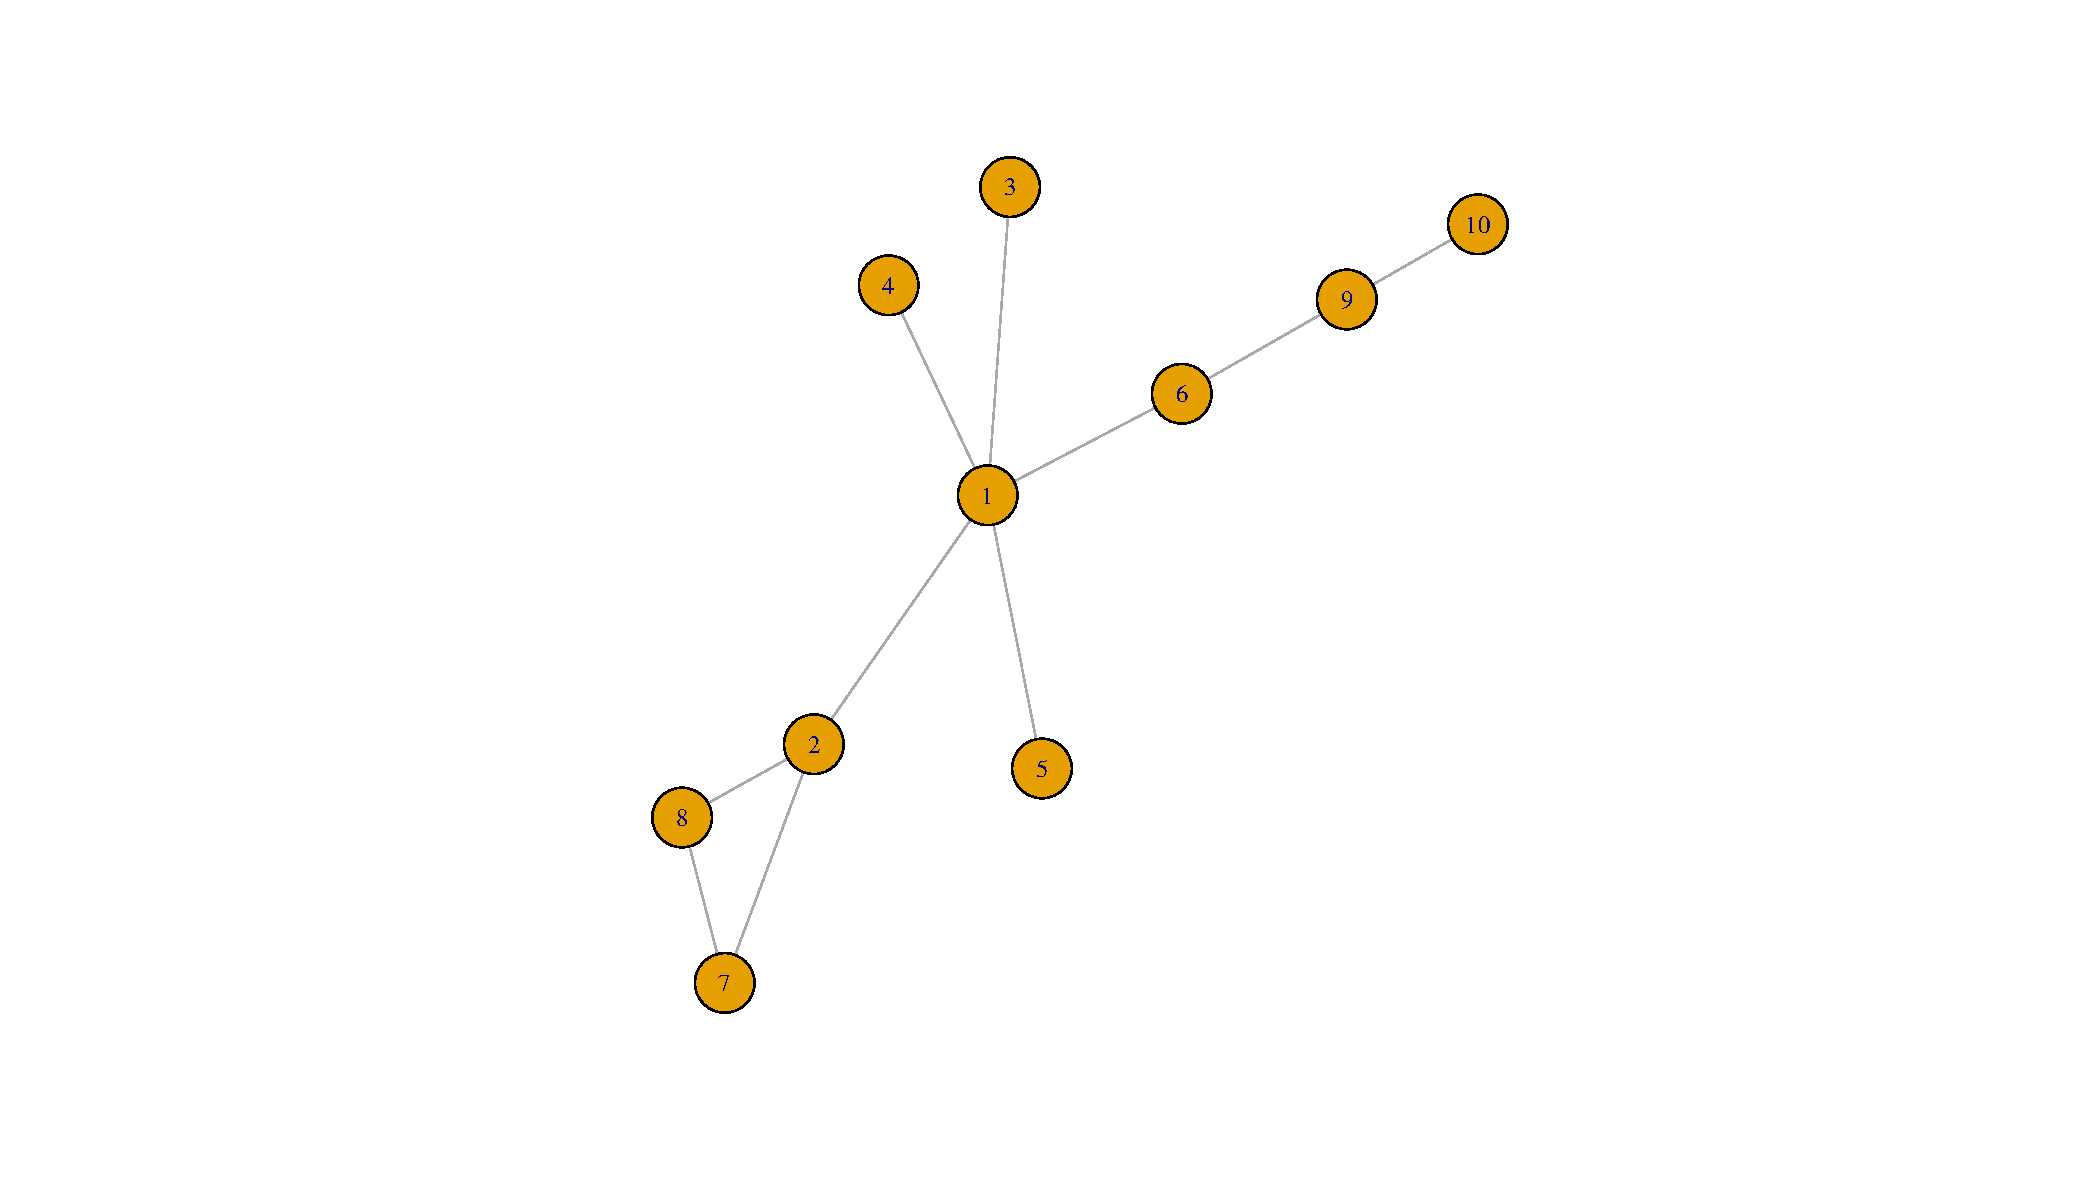
\includegraphics[trim={1 2cm 0 2cm},clip]{thesis_draft_files/figure-latex/unnamed-chunk-1-1} \caption{\label{fig:graph example} A graph configuration. The vertices $i \in \{1,\dots, 10\}$ represent cities each with their own disease counts $Z_{i,t}$. The edges between the graph represent whether the counts between the cities can affect each other. In this example city 1's disease counts at time $t$ are influenced by both its own counts and city 2, 4, 5 and 6's (i.e., every city connected to it) disease counts. City 10's disease counts are only influenced by its own and city 9's.}\label{fig:unnamed-chunk-1}
\end{figure}

We then model the disease count of city \(i\) at time \(t\) as a
function of \(Z_{i,t-1}\) (as before, its own count at time \(t-1\)) as
well as all the count of the cities \(j\) it is connected to,
\(Z_{j,t-1}\). Then the counts at city \(i\) at time \(t\) are modeled
as \[Z_t|Z_{t-1}, G = X_{i, t} + Y_{i,t}|G\] where
\[X_{i,t}: \text{count in city } i \text{ at time step } t \text{, due to endemic factors}, \]
\[Y_{i,t}|G : \text{count in city } i \text{ at time step } t \text{, due to epidemic factors}, \]
\[Z_{i,t}|G = X_{i,t} + Y_{i,t}|G: \text{count in city } i \text{ at time step } t.\]
As before we have the epidemic component as
\(X_{i,t} \sim\text{Pois}(\nu_t)\). For the epidemic component we now
include the additional counts from connected cities as

\[Y_{i,t}|G \sim ~ \text{Pois}\big(\lambda_t\sum_{j\neq i}^{N_v}Z_{j,t-1}1[e_{ij}=1]+ \lambda_tZ_{i,t-1}\big)|G, \]
where \(\lambda_t\sum_{j\neq i}^{N_v}Z_{j,t}1[e_{ij}=1]\) are the counts
from all cities connected to city \(i\). Then the epidemic component for
city \(i\) is the sum of all counts in every city \(j\) connected to
\(i\) in addition to the counts in city \(i\).

\hypertarget{migration}{%
\subsection{Migration}\label{migration}}

One issue with this model is that connecting two isolated cities
essentially doubles the infectivity parameter, since we include the
counts from both cities. In this formulation a connection between two
cities is equivalent to treating them as a single city. To make the
model more realistic, a migration parameter \(m \in (0,1)\) is
introduced so

\[Y_{i,t}|G \sim ~ \text{Pois}\big(m\lambda_t\sum_{j\neq i}^{N_v}Z_{j,t-1}1[e_{ij}=1]+ \lambda_tZ_{i,t-1}\big)|G.\]

The migration parameter \(m\) is then the fraction of counts in city
\(j\) that can cause infections in city \(i\), where \(m = 1\) is
equivalent to the previous model where all incidences in city \(j\) are
counted, whereas when \(m = 0\), no incidences are counted and the model
is equivalent to all cities \(i,j\) not being connected in graph \(G\)
(i.e, \(\{i,j\} \notin E(G)\))

\hypertarget{bayesian-inference}{%
\section{Bayesian Inference}\label{bayesian-inference}}

In Bayesian analysis, we aim to estimate the posterior distribution of
the parameters which we can calculate via Bayes' theorem:
\[ P(\theta|D) = \frac{P(D|\theta)P(\theta)}{P(D)}.\] \(P(\theta|D)\) is
the posterior distribution of the parameters, \(\theta\), given the data
\(D\). \(P(D|\theta)\) is the probability of the data \(D\) given the
parameter value \(\theta\). \(P(\theta)\) is the prior distribution of
\(\theta\) and represents the belief that the parameters will take
certain values before seeing the data. If we have little prior
information about a parameter, we can choose an uninformative prior to
reflect that ignorance. \(P(D)\) is the probability of the data
marginalized over the parameter space. One issue with Bayesian
estimation is finding the \(P(\text{D})\) term, which requires
computation of \(\int P(\text{D}|\theta)P(\theta)\) over the entire
parameter space. With many parameters, this integral is typically
analytically intractable. To handle this Markov chain Monte-Carlo
methods are used which we discuss in section
\protect\hyperlink{methods}{Methods/Implementation}.

We now specify the priors of the two-component and graph portions of the
model.

\hypertarget{priors-for-lambda-gamma-k-and-vectheta}{%
\subsection{\texorpdfstring{Priors for \(\lambda\), \(\gamma\), \(K\)
and
\(\vec{\theta}\)}{Priors for \textbackslash{}lambda, \textbackslash{}gamma, K and \textbackslash{}vec\{\textbackslash{}theta\}}}\label{priors-for-lambda-gamma-k-and-vectheta}}

The prior distribution for the \(\gamma\) parameters is Normal with
variance \(\sigma^2 = 3^2\) to describe an uninformative prior:

\[\gamma_i \sim N(0, 3), i \in \{0,1,2\}.\]

Since the \(\lambda\) values parameterize a Poisson distribution we set
the prior to be

\[ \lambda^{(k)} \sim \text{Gamma}(1, 1),\ k \in \{1, \dots, K + 1\}. \]

The \(\text{Gamma}(1, 1)\), is selected since it's the conjugate prior
of the Poisson. If \(\text{Gamma}\) is interpreted as the sum of
exponentials, then the shape = 1, rate = 1 parameterization represents
seeing a single occurence in 1 unit of time and also represents an
uninformative prior. An uninformative prior is important when we later
incorporate a graph since the magnitude of the \(\lambda_i\)'s can vary
with the connectivity of the graph.

The number of change points \(K\) takes values in \(\{1,\dots,N\}\)
where \(N\) is the total number of time points of counts collected. In
the Held et al. (\protect\hyperlink{ref-held_two-component_2006}{2006})
paper the number of change points is uniformly distributed
\(P(K = k) = 1/N\) representing uncertainty in the number of change
points. This is changed to \[K \sim \text{Pois}(2)\] representing that
idea that the disease count data is already of interest due to a
potential change in the infectivity of the disease.
\(K \sim\text{Pois}(2)\) places the highest mass on \(K = 2\) change
points which can capture a spike in disease counts (as seen in the
simulated data) before returning to a baseline endemic rate. It also
places mass on \(K = 1\) (e.g.~capturing a long term decrease in
infectivity due to intervention) and \(K = 3\) change points. It also
acts as a regularizer to help reduce overfitting the count time series
where each time point is given a unique \(\lambda_t\) value.

The probability of a specific location for a change point given the
number of change points is uniformly distributed among all the possible
change points, \[P(\theta|K=k) = \binom{N}{k}^{-1}.\] Then the
unnormalized posterior is then the product of the likelihood and the
priors,
\[ P(\theta, K, \lambda^{(1)}, \dots, \lambda^{(K+1)}, \gamma_0, \gamma_1, \gamma_2|Z)  \propto \]
\[\prod_{t=1}^N P(Z_t|Z_{t-1},\theta, K, \lambda^{(1)}, \dots, \lambda^{(K+1)}, \gamma_0, \gamma_1, \gamma_2)P(\theta|K)P(K)\prod_{k=1}^{K+1}P(\lambda^{(k)} )\prod_{i=0}^2P( \gamma_i)  .\]

\hypertarget{graph-prior}{%
\subsection{Graph Prior}\label{graph-prior}}

We model the graph \(G\) modeled as an Erdos-Renyi (ER) random graph. An
Erdos-Renyi random graph has a fixed vertex set
\(V(G) = \{1, \dots, N_v\}\) and is parameterized by \(p \in [0,1]\).
Then an edge \(e_{ij}\) is in the edge set \(E(G)\) with probability
\(p\) independent of every other edge in the graph. That is an ER graph
is parameterized as \(G \sim ER(p)\) and the likelihood of a graph \(G\)
given probability \(p\) on an edge is
\[\begin{aligned} G|p & = \prod_{i,j \in V(G),i \neq j} p^{1[e_{ij}]}(1-p)^{1-1[e_{ij}]} 
\\ & = p^{N_e}(1-p)^{\binom{N_v}{2}-N_e} \end{aligned}\] where \(N_e\)
is the number of edges.

We then place a prior on \(p\) as \(p \sim \text{Unif}(0,1)\)
representing a uncertainty about the sparseness of the graph. Now
computing the marginal probability of a graph we find
\[ \begin{aligned} P(G)  & = \int_0^1  P(G,p)dp   = \int_0^1 P(G|p)P(p)dp \\ 
&= \int_0^1 p^{N_e}(1-p)^{\binom{N_v}{2}-N_e}*1*dp = \frac{1}{(\binom{N_v}{2}+1) \binom{\binom{N_v}{2}}{N_e} },  \end{aligned}\]
where \(\binom{\binom{N_v}{2}}{N_e }\) is
\(\binom{N_v}{2} \text{ choose } N_e\) and this calculation is used to
induce the prior on the graph. It may be desirable to place a \(Beta\)
prior in \(p\) with higher mass on lower probabilities.

\hypertarget{posterior}{%
\subsection{Posterior}\label{posterior}}

To summarize, the posterior distribution is proportional to the product
of the likelihood and the priors of the graph and non-graph parameters

\[ P(\vec{\theta}, K, \lambda^{(1)}, \dots, \lambda^{(K+1)}, \gamma_0, \gamma_1, \gamma_2, G,p|Z)  \propto \]
\[\begin{aligned}\prod_{i=1}^{N_v}\prod_{t=1}^N P(Z_{i,t}|Z_{t-1},\theta, K, \lambda^{(1)}, \dots, \lambda^{(K+1)}, \gamma_0, \gamma_1, \gamma_2,G,p)*\\P(\theta|K)P(K)\prod_{k=1}^{K+1}P(\lambda^{(k)} )\prod_{i=0}^2P( \gamma_i)P(G|p)P(p), \end{aligned} \]

where \(\vec{\theta}\) is a \(K\) dimensional vector of locations of
change points (and takes values in \(\{1,\dots,N\}\) where \(n\) is end
of the time series); \(\lambda^{(1)}, \dots, \lambda^{(K+1)}\)
parameterize the epidemic component at the corresponding change points;
\(\gamma_0, \gamma_1, \gamma_2\) parameterize the Fourier series that
drives the endemic component; \(G\) is Erdos-Renyi (ER) random graph
that represents the dependencies between cities and \(p \in (0,1)\)
parameterizes the ER graphs and is the probability of an edge being in
the graph.

\hypertarget{metropolis-hastings-algorithm}{%
\subsection{Metropolis-Hastings
Algorithm}\label{metropolis-hastings-algorithm}}

To approximate the posterior distribution, we draw samples from it using
the Metropolis-Hastings algorithm (and its variant, the
Metropolis-Hastings-Green algorithm). The algorithm creates a Markov
Chain whose states are the parameter space and whose stationary
distribution is the posterior distribution. That is the Markov chain
will eventually enter states in proportion to the posterior
distribution.

The algorithm is as follows:

\begin{enumerate}
\def\labelenumi{\arabic{enumi}.}
\item
  Initialize the Markov chain at some state \(\theta_0\)
\item
  From the current state \(\theta\) at time \(n\) propose a new state
  \(j\) according to \(q\). The probability of proposing a transition
  \(\theta \rightarrow \theta^*\) is \(q(\theta^*|\theta)\)
\item
  Compute the acceptance probability
  \[\alpha(\theta^*|\theta) = \min\{1, \frac{P(D|\theta^*)P(\theta^*)}{P(D|\theta)P(\theta)}\frac{q(\theta|\theta^*)}{q(\theta^*|\theta)} \}\]
\item
  Generate \(U \sim \text{Unif}(0,1)\)
\item
  If \(U < \alpha(\theta|\theta^*)\) then accept the move and the
  parameter value at time \(n+1\) is \(\theta_{n+1} = \theta^*\). If
  \(U \geq \alpha(\theta|\theta^*)\) reject the move. Then the chain
  remains in the same state at time \(n+1\) and
  \(\theta_{n+1} = \theta\).
\item
  Repeat steps 1-5 for a large number of iterations.
\end{enumerate}

The fraction \(\frac{q(\theta^*|\theta)}{q(\theta|\theta^*)}\) is known
as the Hastings ratio and is a function of the proposal distribution. It
allows the base Metropolis algorithm (which requires symmetric
proposals) to work for arbitrary \(q\). Then the transition probability
is ratio of the posterior distributions whose denominators, \(P(D)\),
cancels leaving
\(\frac{P(D|\theta^*)P(\theta^*)}{P(D|\theta)P(\theta)}\). The proposal
ratio becomes important in asymmetric proposal distributions which
occurs in some of the graph proposals below. For example if two
parameter \(\theta, \theta^*\) values are equally likely,
\(P(\theta^*|D) = P(\theta|D)\) then the posterior distribution should
have approximately equal frequency of these two states. However if the
proposal distribution proposes entering \(\theta^*\) twice as frequently
as \(\theta^*\) then without the Hastings ratio there would be twice the
frequency of \(\theta^*\), since they're accepted at the same rate but
one is proposed twice is frequently. A similar issue is also seen when
jumping between parameter spaces. To handle this the
Metropolis-Hastings-Green algorithm is introduced which adds an
additional Jacobian term \(|J|\) to handle the change in dimension. This
is described further below.

\hypertarget{two-component-model}{%
\subsection{Two-Component Model}\label{two-component-model}}

\hypertarget{model-checking}{%
\subsection{Model Checking}\label{model-checking}}

\hypertarget{prior-checks}{%
\subsubsection{Prior Checks}\label{prior-checks}}

By setting the likelihood to always equal 1, the posterior is only a
function of the priors

\[\begin{aligned} P(\theta|D) & \propto P(D|\theta)P(\theta) \\ & \propto 1*P(\theta)  \end{aligned} \]
that is the samples returned by the MCMC should be drawn from the prior
distribution. This helps shows that the prior distributions are properly
implemented in the model as well as show potentially unintended
assumptions about the priors. Furthermore, it can help show any issues
with the Hastings computation. Other prior analysis include prior
sensitivity analysis where the effect of different priors on the
posterior distribution are examined. This is less important when the
datasets are large sense the likelihood portion generally dominates the
posterior calculation.

\hypertarget{effective-sample-size}{%
\subsubsection{Effective Sample Size}\label{effective-sample-size}}

The effective sample size is a downward adjustment of the number of
samples drawn from the posterior distribution. Since the samples are not
independent, their overall variance is lower than would be expected from
truly independent samples. To adjust for this the following is used to
estimate the effective sample size

\[ \widehat{n_{eff}} = \frac{mn}{1+ 2\sum_{t=1}^T \widehat{\rho_t}},  \]
where \(m\) is the number of chains, \(n\) is the samples per chain and
\(\widehat{\rho_t}\) is an estimate of the autocorrelation as seen in
Gelman et al. (\protect\hyperlink{ref-gelman_bayesian_2013}{2013}),
pp.~286. The effective sample size can be used to calculate estimates of
the variance of the means of the posterior distributions.

\hypertarget{well-calibrated}{%
\subsubsection{Well-Calibrated}\label{well-calibrated}}

A goal of frequentist statistical inference is to obtain confidence
intervals (CI), where a 95\% CI for a parameter would capture the true
parameter in 95\% of replications.

A credible interval plays a similar role in Bayesian inference. We would
like a 95\% credible interval for a parameter to capture the ``true''
parameter value 95\% of the time. If this is the case, then the model is
considered ``well-calibrated''. To do this for Bayesian models, we draw
samples of the estimated parameters from their prior distributions
\(\theta_{sample_1} \sim P(\theta)\) and then using the sampled
parameters we simulate data according to the likelihood function
\(D_{1} \sim P(D|\theta_{sample_1})\). The model is then used to compute
95\% credible intervals as if it were real data. This process is
repeated for
\((\theta_{sample_2}, D_2), \dots, (\theta_{sample_N}, D_N)\) and their
corresponding credible intervals are collected. We can then compare to
see if the 95\% credible intervals from the \(N\) parameter samples,
covers the true sampled parameter 95\% of the time (Carpenter
\protect\hyperlink{ref-carpenter_bayesian_2017}{2017}; Cook et al.
\protect\hyperlink{ref-cook_validation_2006}{2006}).

\hypertarget{posterior-predictive-checking}{%
\subsubsection{Posterior Predictive
Checking}\label{posterior-predictive-checking}}

If the model is a good fit for the data, then simulating data by
sampling according the posterior distribution, should result in
simulated data that looks similar to the true data. If this is not the
case, the model is potentially inadequate for capturing important
features of the data. This can be done in a qualitative manner where
obviously poor models can be investigated (Gelman et al.
\protect\hyperlink{ref-gelman_bayesian_2013}{2013},pp. 141--159;
Kruschke \protect\hyperlink{ref-kruschke_doing_2014}{2014},pp. 130--131)

\hypertarget{methods}{%
\section{Methods/Implementation}\label{methods}}

Here we describe the Metropolis-Hastings algorithms used to draw samples
from the posterior distributions of the parameters of interest. The
operators generate and evaluate proposals and are implemented as an R
function. Each operator accepts a list of parameters that represents the
current state of the Markov chain, then proposes an new state for a
given parameter (or set of parameters). The function then calculates the
log acceptance ratio and determines whether to accept its proposal or
reject it. It then returns the proposed parameters or returns the
original parameters (if it rejects the proposal). The algorithms are
implemented in base R (R Core Team
\protect\hyperlink{ref-r_core_team_r:_2019}{2019}) with some elements of
the likelihood computation implemented in Rcpp (Eddelbuettel and
François \protect\hyperlink{ref-eddelbuettel_rcpp:_2011}{2011}). Plots
are generated in base R and the bayesplot (Gabry and Mahr
\protect\hyperlink{ref-gabry_bayesplot:_2019}{2019}). Parallel chains
are implemented using doParallel (Corporation and Weston
\protect\hyperlink{ref-corporation_doparallel:_2019}{2019}) and
diagostics done with coda (Plummer et al.
\protect\hyperlink{ref-plummer_coda:_2006}{2006}).

\hypertarget{likelihood-computation}{%
\subsection{Likelihood Computation}\label{likelihood-computation}}

Each operator receives the log-likelihood of its proposal by passing the
proposal to either \texttt{compute\_log\_like()} function or the
\texttt{compute\_log\_like\_diff()} function. The
\texttt{compute\_log\_like()} function returns the unnormalized
log-likelihood of the proposed parameters. This is computationally more
efficient since computing the normalized likelihood of a Poisson
distribution requires the evalution of \(Z_{t}!\) for each data point.
The naive method of computing the entire log-likelihood was used as it
was computationally fast enough on the simulated dataset (without the
graph).

This differs from Held et al.
(\protect\hyperlink{ref-held_two-component_2006}{2006}) and Green
(\protect\hyperlink{ref-green_reversible_1995}{1995}) who perform
separate likelihood computations for each of their three operators:
birth (adding a change point), death (removing a change point) and
changing a \(\lambda\) value. Each of these operators changes only a
portion of the total likelihood computation and as such, it is
computationally more efficient to only compute the ratio of the changes.
For example, let \(\boldsymbol{\theta^*}\) be the proposed change point
vector where \(K^* = K + 1\) (i.e.~a new change point is added). Let
\(m\) be the index of the proposed change point and the rest of the
change points remain the same. Then the only part of the likelihood
computation that changes is in the interval between timepoints
\([\theta_{m-1}, \theta_{m+1})\) and since its the ratio between the
likelihoods of the proposed vs the current parameter set is important,
the parts that remain identical have a likelihood of 1 (or
log-likelihood of 0).

Similar reductions in comptutation can be done following changes in the
graph and are implemented in \texttt{compute\_log\_like\_diff()}. If an
edge \(e^*_{ik}\) is proposed then only \(Y_{i,t}\) and \(Y_{k,t}\) and
the corresponding \(Z\)'s are affected. As such only those two cities
need to be updated.
\[Y^*_{i,t}|G \sim ~ \text{Pois}\big(m\lambda_tZ_{k,t-1} +m\lambda_t\sum_{j=1}^{N_v}Z_{j,t-1}1[e_{ij}\in E(G)]+ \lambda_tZ_{i,t-1}\big) \]
\[Y^*_{k,t}|G \sim  \text{Pois}\big(m\lambda_tZ_{i,t-1} +m\lambda_t\sum_{j=1}^{N_v}Z_{j,t-1}1[e_{ij}\in E(G)]+ \lambda_tZ_{i,t-1}\big) \]
\[\begin{aligned} Y_{j,t}|G &\sim \text{Pois}\big(m\lambda_t\sum_{l=1}^{N_v}Z_{j,t-1}1[e_{jl}\in E(G^*)]+ \lambda_tZ_{i,t-1}\big)\\ & \sim  \text{Pois}\big(m\lambda_t\sum_{l=1}^{N_v}Z_{j,t-1}1[e_{jl}\in E(G)]+ \lambda_tZ_{i,t-1}\big) \end{aligned}\]

Then the likelihood ratio can be computed as (dropping conditioning
notation for clarity)

\[ \frac{P(Z^*_{i,t})P(Z^*_{k,t})}{P(Z_{i,t})P(Z_k,t)}\frac{\prod_j P(Z_{j})}{\prod_{j}P( Z_{j})} = \frac{P(Z^*_{i,t})P(Z^*_{k,t})}{P(Z_{i,t})P(Z_k,t)} \]
This lets the computational complexity stay constant with respect to the
size of the graph. This is currently implemented for the
\texttt{add\_edge\_op()} and \texttt{del\_edge\_op()} operators.

\hypertarget{change_gamma-change_lambda}{%
\subsection{\texorpdfstring{\texttt{change\_gamma()},
\texttt{change\_lambda()}}{change\_gamma(), change\_lambda()}}\label{change_gamma-change_lambda}}

The gamma and lambda parameters are updated in blocks via a standard
Metropolis-Hastings step (Gelman et al.
\protect\hyperlink{ref-gelman_bayesian_2013}{2013},p. 280). The gamma
and lambda proposals are each drawn from Normal distributions centered
at the current parameter values. That is the proposed parameter vectors
\(\gamma^*\) and \(\lambda^*\) are drawn from
\(\text{Norm}(\gamma, \sigma_\gamma)\) and
\(\text{Norm}(\lambda, \sigma_\lambda)\). The variance of the
distributions is scaled as \(\sigma_\gamma\) and \(\sigma_\lambda\)
which are hand selected to improve mixing.

Since the Normal distribution is symmetric, the Hastings ratio is 1 so
the acceptance ratio is the ratio of the likelihoods between the current
and proposed steps.

One potential issue is that gamma and lambda are used to compute the
parameter of a Poisson distribution, but the Normal distribution
proposals could potentially propose invalid parameter values. To remedy
this, the proposal operator checks to see whether the proposed parameter
value is valid (in this case positive) and automatically rejects the
proposed state (staying in the current state). This could be
side-stepped by using a non-symmetric proposal distribution such as
log-normal or a truncated normal and an adjustment of the Hastings ratio
to compensate for the asymmetry. However this does not seem to be an
issue in the simulated cases, the initial values are positive and the
jump (\(\sigma\)) size is small enough not to propose negative values.

\hypertarget{change_theta}{%
\subsection{\texorpdfstring{\texttt{change\_theta()}}{change\_theta()}}\label{change_theta}}

This operator proposes a new location for one of the current change
points \(\theta_1,\dots, \theta_K\). A change point
\(\theta_k, k \in \{1, \dots, K\}\) is selected uniformly at random from
all current change points. Then the proposed location \(\theta_k^*\) is
selected from values between
\(\{\theta_{k-1}+1,\dots, \theta_{k+1}-1\}\) uniformly at random. For
\(\theta_1\) and \(\theta_k\) the proposed values are from
\(\{0,\dots, \theta_1-1\}\) and \(\{\theta_K+1,\dots, N\}\)
respectively.

The \(\lambda\) are then updated to match the newly proposed location
as:

\[ \lambda_t =  \begin{cases} \lambda^{(1)} & t < \theta_0 \\
\lambda^{(k^*)}, & \theta_{k^*} \leq t < \theta_{(k^*-1)} \\
\lambda^{(K+1)}, & t \geq \theta_K \end{cases}\]

Since the proposal is generated uniformly at random between
\(\theta_{k-1}\) and \(\theta_{k+1}\) the proposal probability is
\[q(\theta_{k^*}|\theta_k) = \frac{1}{\theta_{k+1}-\theta_{k-1}-2} = q(\theta_k|\theta_k^*)\].
Furthermore the \(\lambda\) values are deterministically generated from
current \(\lambda_k\) values and the \(\theta_k^*\) values. The Hastings
ratio is then 1 and the acceptance rate is the ratio of the likelihoods.

\hypertarget{birthdeath_theta-and-reversible-jump-mcmc}{%
\subsection{\texorpdfstring{\texttt{birth/death\_theta()} and Reversible
Jump
MCMC}{birth/death\_theta() and Reversible Jump MCMC}}\label{birthdeath_theta-and-reversible-jump-mcmc}}

The \texttt{birth\_theta()} and \texttt{death\_theta()} operators allow
for an increase and decrease in the number of change points. Then the
parameter space can jump between a collection of possible models
\(\{M_K, K \in \{0,1,\cdots,n-1\}\}\) where \(K\) indexes the number of
change points. However models from different \(M_K\)'s have different
dimensions of \(\vec{\theta}\) and the likelihoods are not directly
comparable (since they are not defined on the same probability space).
To handle this we use a Reversible Jump MCMC (RJMCMC) as proposed in
Green (\protect\hyperlink{ref-green_reversible_1995}{1995}).

\hypertarget{birth_theta}{%
\subsubsection{\texorpdfstring{\texttt{birth\_theta()}}{birth\_theta()}}\label{birth_theta}}

For a birth step a new change point is chosen uniformly at random from
all possible time steps \(\{1,\dots,N\}\) that aren't currently change
points \(\{\theta_1,\dots,\theta_K\}\) and then added to the current set
of change points

\begin{enumerate}
\def\labelenumi{\arabic{enumi}.}
\item
  Draw \(u \sim Unif(0,1)\)
\item
  The following proposals for the new \(\lambda_1\) and \(\lambda_2\)
  values are from
  \[\lambda_1 = \lambda_0*(\frac{u}{1-u})^{(\theta_1-\theta_0)/(\theta_2-\theta_0)}\]
  \[\lambda_2 = \lambda_0*(\frac{1-u}{u})^{(\theta_2-\theta_1)/(\theta_2-\theta_0)}\]
  That is the new \(\lambda\) values are a compromise between the
  original value \(\lambda_0\) of the interval that was split. This
  compromise is a function of the location of the split in the interval.
\item
  In order to determine the acceptance probability for the proposal, the
  corresponding death move must also be determined. In death move a
  current change point is selected uniformly at random and then removed.
  Then the \(\lambda\) values are changed deterministically (as
  described later).
\end{enumerate}

The \(P(birth)\) and \(P(death)\) are the probabilities of proposing a
birth and death step and are selected such that \(P(birth) = P(death)\).
The \(q_{(K+1\rightarrow K)}(\theta|\theta^*)\) term is transition
probability from a parameter state with \(K\) to \(K+1\) change points.
The probability of being in the proposed state \(\theta^*\) and
proposing jumping back to the current state \(\theta\) is the
probability of selecting the newly added change point \(\theta_{k^*}\)
and deleting it. This occurs with probability \(1/(K+1)\) since the
change points are selected uniformly at random and there are \(K+1\)
change points in the proposed state. Similarly the probability of the
current proposal state is \(1/(N-K)\) since there are \(N-K\) possible
timesteps to add. Since \(u \sim U(0,1)\) then \(P(u) = 1\) and the
reverse move is deterministic so its probability is also 1 (and omitted
from the equation). Finally the Jacobian is given by
\[ |J_{birth}| = \frac{(\lambda_1 + \lambda_2)^2}{\lambda_0}\] .

Then the new acceptance ratio is
\[\alpha_{birth}(\theta^*|\theta) = \frac{P(death)}{P(birth)}\frac{q_{(K+1\rightarrow K)}(\theta|\theta^*)}{q_{(K\rightarrow K + 1)}(\theta^*|\theta)*P(u)}|J_{birth}|,\]
where
\[  \frac{P(death)}{P(birth)}\frac{q_{(K+1\rightarrow K)}(\theta|\theta^*)}{q_{(K\rightarrow K + 1)}(\theta^*|\theta)*P(u)} \]
\[= 1*\frac{\frac{1}{K+1}}{\frac{1}{N-K}*1} = \frac{N-K}{K+1} \]

\hypertarget{death_theta}{%
\subsubsection{\texorpdfstring{\texttt{death\_theta()}}{death\_theta()}}\label{death_theta}}

For the death proposal we randomly select any of the current change
points uniformly at random and remove it. Then the two \(\lambda\)
values associated with the removed change point (call them \(\lambda_1\)
and \(\lambda_2\) to match the above notation) are recombined
deterministically as

\[ \lambda_0 =\lambda_1^{\frac{\theta_m-\theta_{m-1}}{\theta_{m+1}-\theta_{m-1}}}*\lambda_2^{\frac{\theta_{m+1}-\theta_{m}}{\theta_{m+1}-\theta_{m-1}}} \]
where \(\theta_m\) is the theta value that was removed and \(\lambda_0\)
is the new \(\lambda\) value for the merged interval.

The probability of proposing the death of change point \(\theta_m\) is
\(1/K\) since it is chosen uniformly at random from
\(\boldsymbol{\theta}\) which has dimension \(K\). The
\(q_{(K-1\rightarrow K)}(\theta|\theta^*)\) term is the probability of
adding back the change point. Since the change points are birthed
uniformly at random from all change point not currently in the
\(\boldsymbol{\theta^*}\) vector, the probability of birthing the
\(\theta_m\) that was deleted which is \(1/(N-(K-1)) = 1/(N-K+1)\) And
the Jacobian is
\[|J_{death}| = \frac{1}{|J_{birth}|} = \frac{\lambda_0}{(\lambda_1 + \lambda_2)^2}\]
since the function is invertible.

Then the acceptance rate is computed as
\[\alpha_{death}(\theta^*|\theta) = \frac{P(birth)}{P(death)}\frac{q_{(K-1\rightarrow K)}(\theta|\theta^*)*P(u)}{q_{(K\rightarrow K - 1)}(\theta^*|\theta)}\frac{1}{|J_{death}|}\]
where
\[ \frac{P(birth)}{P(death)}\frac{q_{(K-1\rightarrow K)}(\theta|\theta^*)*P(u)}{q_{(K\rightarrow K - 1)}(\theta^*|\theta)} = 1*\frac{\frac{1}{N-K+1}}{\frac{1}{K}} = \frac{K}{N-K+1}.\]

\hypertarget{graph-proposals}{%
\subsection{Graph Proposals}\label{graph-proposals}}

The data structure for the graph is an adjacency list and is implemented
using a list of numeric vectors in R. While not a true hashmap,
numerically indexing the list allows for near \(O(1)\) look-ups (Horner
\protect\hyperlink{ref-horner_hash_2015}{2015}). To make proposals in
the graph space the following operators are used.

\hypertarget{add_edge_op-and-delete_edge_op}{%
\subsection{\texorpdfstring{\texttt{add\_edge\_op()} and
\texttt{delete\_edge\_op()}}{add\_edge\_op() and delete\_edge\_op()}}\label{add_edge_op-and-delete_edge_op}}

The \texttt{add\_edge\_op()} functions proposes adding an edge to the
graph by sampling uniformly at random from all edges not currently in
the graph. Let \(N_v\) be the number of vertices (cities) in the graph
and \(N_e\) the current number of edges. Then the probability of
selecting an edge to add is \(2/(N_v(N_v-1) - 2N_e)\) by symmetry. This
is determined as follows:

\begin{enumerate}
\def\labelenumi{\arabic{enumi}.}
\item
  \(N_v(N_v-1)\) is the total possible size of the adjacency list and
  \(N_e\) is the number of unique edges currently in the list. Then
  \(N_v(N_v-1) - 2N_e\) is the remaining ``slots'' in the adjacency
  list.
\item
  We draw uniformly at random \(A \in \{1,\dots,N_v(N_v-1) - 2N_e\}\)
  which represents an index of the edges not present in the graph.
\item
  Now we interate along the adjacency list \texttt{adj} whose length is
  the number of vertices \(N_v\). Starting from \(i = 1\) if
  \(A_i <= N_v - \text{length}(\text{adj}[i])\) then we know that the
  edge to be added is in \(\text{adj}[i]\) and we can search for the
  correct edge in \(O(|V|)\).
\item
  Otherwise if \(A_i > N_v - \text{length}(\text{adj}[i])\) then we
  recompute \(A_{i+1} = A_i - N_v + \text{length}(\text{adj}[i])\)
  increment \(i = i + 1\) and repeat.
\end{enumerate}

Then \(q(G^*_{N_e+1}|G_{N_e})\) the probability of proposing adding that
particular edge occurs with probability \(2/(N_v(N_v-1) - 2N_e)\), since
\(A_0\) is chosen uniformly at random from
\(\{1,\dots,N_v(N_v-1) - 2N_e\}\) and each edge \(e_{ij}\) is
represented twice (once in \text{adj}{[}i{]}: \{\dots,j,\dots\}) and
again in \(\text{adj}[j]: \{\dots,i,\dots\}\).

An edge is deleted by randomly sampling from the adjancency list. The
probability of \(q(G_{N_e}|G^*_{N_e+1})\) of deleting the edge (given
the graph where the proposed edge was added) occurs with probability
\(2/2(N_e+1) = 1/(N_e+1)\). Then the Hastings ratio for adding an edge
is

\[\frac{q(G_{N_e}|G^*_{N_e+1})}{q(G^*_{N_e+1}|G_{N_e})} = \frac{\frac{1}{N_e+1}}{\frac{2}{N_v(N_v-1) - 2N_e}} = \frac{N_v(N_v-1) - 2N_e}{2(N_e+1)},\]
and the Hastings ratio for removing an edge is given by

\[  \begin{aligned} \frac{q(G_{N_e}|G^*_{N_e-1})}{q(G^*_{N_e-1}|G_{N_e})} & = \frac{\frac{2}{N_v(N_v-1) - 2(N_e-1)}}{\frac{1}{N_e}} \\ &= \frac{2N_e}{N_v(N_v-1) - 2(N_e-1)}. \end{aligned}\]

\hypertarget{degree_preserving}{%
\subsection{\texorpdfstring{\texttt{degree\_preserving()}}{degree\_preserving()}}\label{degree_preserving}}

The degree preserving swap was implemented to allow changes to the graph
structure while maintaining the degree of each vertex. This is because
with large migration rates, the degree of the cities strongly influences
the likelihood. Let's assume that the migration rate \(m = 1\), then in
Figure \ref{fig:deg_pre}, city 5 and 2 have double the counts of cities
1, 3, 4, and 6. Let's also assume that the configuration on the right is
the true graph. If the MCMC algorithm proposes the graph on the left
first, to get to the graph on the right would require say, disconnecting
\(1-5\) as seen in the middle. With such a high migration rate, the
cities \(5\) and \(2\) would never be swapped (it would require
transitioning to a graph where city \(5\) would have degree \(2\) and
city \(1\) degree 0). The degree preserving swap handles directly
swapping between the left and right graphs without passing through the
middle.

This was implemented by selecting two edges (v11, v12) and (v21, v22)
and attempting to form the edges (v11, v22) and (v12, v21). If both
edges are not already in the graph then the swap is made. If either or
both edges exists, then the proposed swap is rejected. Since the
proposed swap is reversed by randomly selecting (v11, v22) and (v12,
v21), the Hastings ratio is 1 and the acceptance ratio is the ratio of
the likelihoods.

\begin{figure}

{\centering 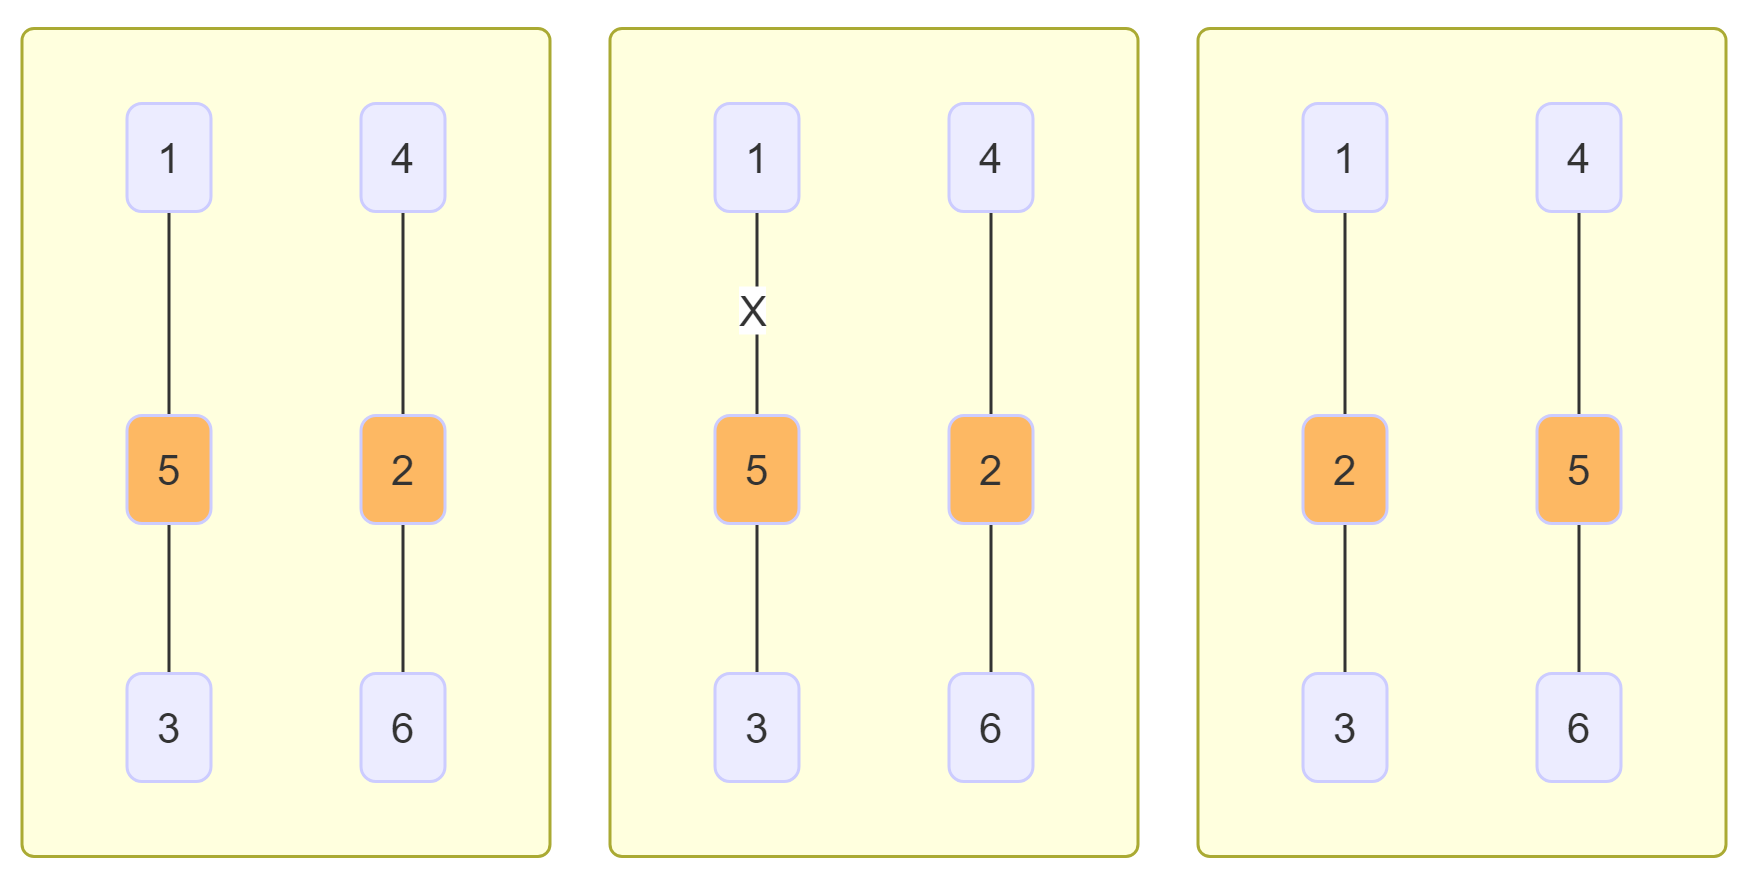
\includegraphics[width=0.75\linewidth]{C:/repos/disease_sim/degree_pre_diag} 

}

\caption{\label{fig:deg_pre}An example graph configuration that might necessitate a degree preserving swap. \textbf{Left} and \textbf{right}: two configurations of graphs whose vertices have the same degree, \textbf{middle}: a potential intermediary proposal. With one-step edge adding and deleting the likelihood of switching between these two graph is low if the migration rate is high enough.}\label{fig:unnamed-chunk-2}
\end{figure}

\hypertarget{rewire}{%
\subsection{\texorpdfstring{\texttt{rewire()}}{rewire()}}\label{rewire}}

The \texttt{rewire()} operator's goal is similar to that of the
\texttt{degree\_preserving()} operator. It tries to select an edge,
delete it, and then reattach one of the vertices randomly. The operator
selects uniformly at random an edge (v1, v2) and deletes it from the
adjacency list. It then randomly samples a vertex v3 and forms the edge
(v2, v3). Since the reverse move is selecting the edge (v2, v3) and then
rewiring (v1, v2), the Hastings ratio is 1.

\hypertarget{change_migration}{%
\subsection{\texorpdfstring{\texttt{change\_migration()}}{change\_migration()}}\label{change_migration}}

The migration proposal is drawn from a
\(\text{Unif}\sim (m-0.01, m+0.01)\). Since the Uniform distribution is
symmetric, the Hastings ratio is 1 so the acceptance ratio is the ratio
of the likelihoods between the current and proposed steps. The Uniform
was chosen over the Normal, since the variance of the Normal is larger
and can propose much larger jumps. This appears to cause many rejections
which slows the exploration of the space.

\hypertarget{results-and-discussion}{%
\section{Results and Discussion}\label{results-and-discussion}}

\hypertarget{prior-checks-1}{%
\subsection{Prior Checks}\label{prior-checks-1}}

Here the likelihood ratio was set to 1 so the only factor in accepting
or rejecting a state was the priors. As such we would expect to see the
posterior distributions of each parameter to be their respective prior
distributions. This helps check that the Hastings ratio is calculated
correctly and the implementation of the operators (excluding the
likelihood) are correct. The following data was collected by running
100,000 iterations (thinned to 10,000 samples) of proposing to update
either the \(\lambda\) vector, \(\gamma\) vector, adding a change point
(\(K \rightarrow K + 1\)) or removing a change point
(\(K \rightarrow K - 1\)).

\begin{figure}
\centering
\includegraphics{thesis_draft_files/figure-latex/lam_gamma_prior_check, prior_checks_2c-1.pdf}
\caption{\label{fig:pc2c} Prior Checks for \(\gamma\) and \(\lambda\).
Only 3 \(\lambda\) values are displayed. The KDE smoothed distribution
of values are plotted against the true density values of the priors
(that is \(P(\lambda) \sim \text{Gamma}(1,1)\) and
\(P(\gamma) \sim \text{Norm}(0,3)\). The differences appear to be due to
sampling and smoothing. \(\lambda_1\) shows the least agreement with the
prior.}
\end{figure}

The priors seen here are \[\vec\lambda \sim \text{Gamma}(1,1),\]
\[\vec\gamma \sim \text{Norm}(0,3),\] \[K \sim \text{Unif}(0,N).\]

In Figure \ref{fig:pc2c} we have plots of the samples of the \(\lambda\)
values (first 3) and the \(\gamma\) values. Each is overlayed with the
density of their respective priors in red. Overall there appears to be a
good match between the sampled values and their prior distributions.

In Figure \ref{fig:pois_hist} we have a frequency histogram of the
sampled values of \(K\) (the number of change points) overlayed with a
red circle. The red circle represents the appropriate density value from
the prior distribution of \(K\). Overall we see a good qualitative fit
between the values sampled from the posterior and the prior
distribution.

\begin{figure}
\centering
\includegraphics{thesis_draft_files/figure-latex/prior_check_k-1.pdf}
\caption{\label{fig:pois_hist} Sample probabilities of \(K\) overlayed
with true probabilities. Overall this shows a good agreement between the
sample probabilities and the true probabilties.}
\end{figure}

\hypertarget{inference-on-simulated-data}{%
\subsection{Inference on Simulated
Data}\label{inference-on-simulated-data}}

The following simulation parameters are taken from Held et al.
(\protect\hyperlink{ref-held_two-component_2006}{2006})'s simulations.

\pagebreak

\begin{longtable}[]{@{}cc@{}}
\toprule
parameters & simulation values\tabularnewline
\midrule
\endhead
K: number of changespoints & 2\tabularnewline
\(\boldsymbol{\lambda}\): epidemic parameters & 0.7, 1.2,
0.7\tabularnewline
\(\boldsymbol{\gamma}\): endemic parameters & log(10), 0.5,
1.5\tabularnewline
\(\boldsymbol{\theta}\): change points & 39, 49\tabularnewline
\bottomrule
\end{longtable}

\begin{figure}
\centering
\includegraphics{thesis_draft_files/figure-latex/gam_lam_traces_plot-1.pdf}
\caption{\label{fig:lam_trace} Trace plots for \(\boldsymbol{\gamma}\)
and \(\boldsymbol{\theta}\). The trace plots seem relatively well mixed.
The autocorrelation is likely a function of the correlation between the
each set of \(\boldsymbol{\gamma}\) and \(\boldsymbol{\theta}\)
respectively. Thinning could potentially reduce the autocorrelation
between sample draws.}
\end{figure}

Figure \ref{fig:lam_trace} are trace plots, which are time series of the
parameter draws. Typically a ``good'' trace plot shows no obvious
autocorrelation (which can indicate a proposal step that is too small)
or flat portions (proposal steps that are too large). Trace plots with
these patterns indicate that the sampler has not converged to the
posterior distribution of the parameter. ``Tuning'' or adjusting the
proposal jump size can help fix these patterns, with the end goal of
being able to efficiently explore the posterior distribution of the
parameter (Gelman et al.
\protect\hyperlink{ref-gelman_bayesian_2013}{2013},p. 296). The trace
plots for the \(\gamma\) parameters seem to have a slight pattern
particularly in the \(\gamma_0\) trace plot.

\begin{figure}
\centering
\includegraphics{thesis_draft_files/figure-latex/gamma_cor-1.pdf}
\caption{\label{fig:cor_gammas} Plots of \(\gamma_0\) vs \(\gamma_1\)
and \(\gamma_0\) vs \(\gamma_2\). Each point represents the
corresponding parameter value at the same sample draw, i.e., the values
of each parameter when the sample was accepted. The strong correlation
between the parameters can lead to poor mixing. Note the tails are due
to the initial values of the MCMC chain.}
\end{figure}

This is likely due to the correlation (see Figure \ref{fig:cor_gammas} )
between \(\gamma_0\), \(\gamma_1\) and \(\gamma_2\) due to their nature
of parameterizing a cyclical function. The same is true for the
\(\theta\) parameters; they are constrained such that
\(\theta_1 < \theta_2 < \theta_3\). The dependence can cause inefficient
sampling by proposing moves that are outside these narrow
regions/combinations of parameter values (Turner et al.
\protect\hyperlink{ref-turner_method_2013}{2013}). This autocorrelation
seen in the trace plots could possibly be reduced via thinning
i.e.~taking every \(k\) samples instead of every sample. Gelman et al.
(\protect\hyperlink{ref-gelman_bayesian_2013}{2013}) mentions that they
have found it useful to store no more than a total of \(1000\)
iterations.

The \(\theta_3\) trace plot is of note because it is only valid for when
\(K = 3\); the \(\theta_3\) does not exist otherwise.

\begin{figure}

{\centering 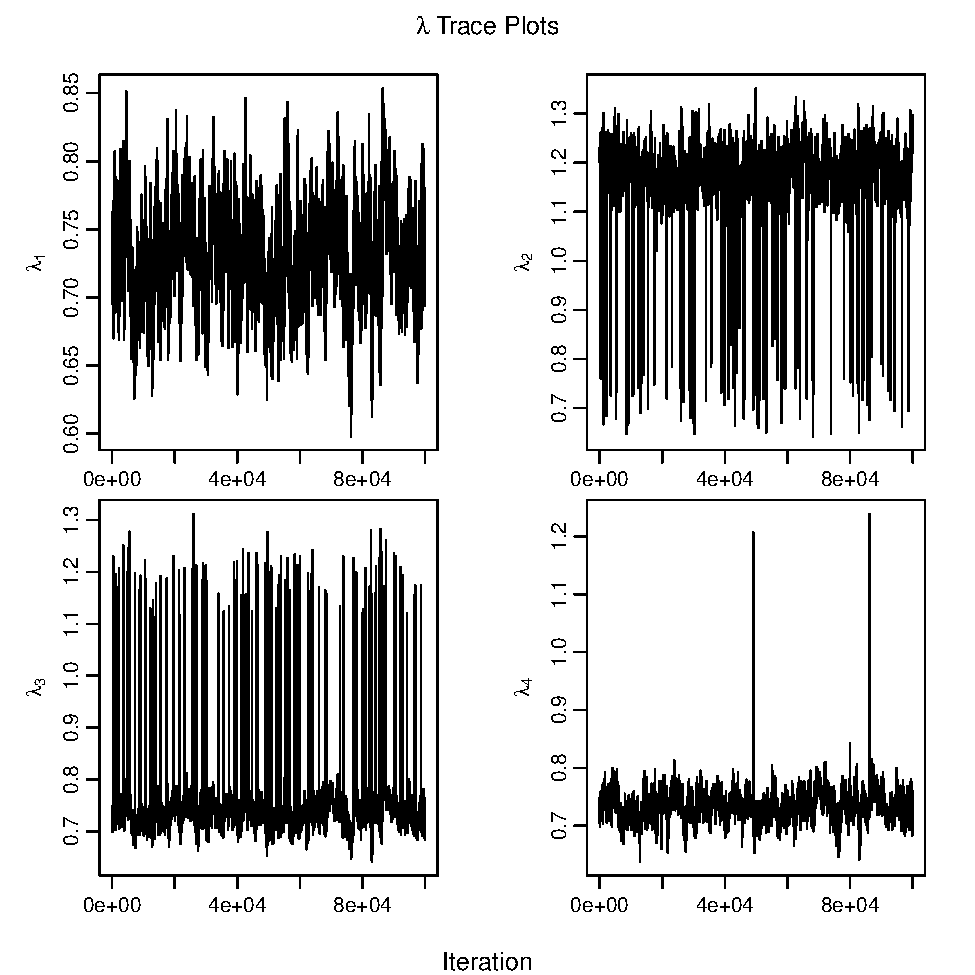
\includegraphics[height=0.41\textheight]{thesis_draft_files/figure-latex/lambda_traces-1} 

}

\caption{Trace plots for all $\lambda$ values. Overall the trace plots show that the samplers are mixing well with some minor autocorrelation that could potentially be resolved with thinning or more samples. The raw trace plots include the $\lambda$ values when there are 3 and 4 separate $\lambda$'s and is the cause of the random jumps.}\label{fig:lambda_traces}
\end{figure}

The \(\boldsymbol{\lambda}\) trace plots show that the \(\lambda_2\) and
\(\lambda_3\) traces appear to jump tightly around \(1.2\) and \(0.7\)
respectively while also jumping to \(0.7\) and \(1.2\) respectively.
This is an artifact of the dimension change in the model. When
\(K = 2\), \(\lambda_2\) is tightly fixed around \(1.2\) and
\(\lambda_3\) at \(0.7\) but when \(K = 2\), \(\lambda_3\) can take the
role of fitting the outbreak while \(\lambda_4\) models to the return
\(0.7\), the baseline.

\begin{figure}

{\centering \includegraphics[height=0.41\textheight]{thesis_draft_files/figure-latex/filtered_traces-1} 

}

\caption{Trace plots filtered for K = 2 and K = 3 showing how the different number of change points affects the traces of the individual $\lambda$ values.}\label{fig:filtered_traces}
\end{figure}

\begin{figure}
\centering
\includegraphics{thesis_draft_files/figure-latex/hist_samples_2c-1.pdf}
\caption{\label{fig:2c_dens} Histogram of posterior samples from \(K\),
\(\lambda_1\), \(\lambda_2\), \(\lambda_3\), \(\lambda_4\), \(\theta_1\)
and \(\theta_2\).}
\end{figure}

Figure \ref{fig:2c_dens} shows the histograms of the \(\lambda\) and
\(\gamma\) samples

\begin{longtable}[]{@{}ccc@{}}
\toprule
parameters & lower & upper\tabularnewline
\midrule
\endhead
K & 2 & 2\tabularnewline
\(\boldsymbol{\lambda_1}\) & 0.67 & 0.82\tabularnewline
\(\boldsymbol{\lambda_2}\) & 1.09 & 1.29\tabularnewline
\(\boldsymbol{\lambda_3}\) & 0.69 & 0.80\tabularnewline
\(\boldsymbol{\gamma_0}\) & 1.95 & 2.50\tabularnewline
\(\boldsymbol{\gamma_1}\) & 0.36 & 0.67\tabularnewline
\(\boldsymbol{\gamma_2}\) & 1.28 & 1.68\tabularnewline
\(\boldsymbol{\theta_1}\) & 39 & 49\tabularnewline
\(\boldsymbol{\theta_2}\) & 39 & 49\tabularnewline
\bottomrule
\end{longtable}

\pagebreak

\hypertarget{graph-inference-on-fixed-two-component-model}{%
\subsection{Graph Inference on Fixed Two-Component
Model}\label{graph-inference-on-fixed-two-component-model}}

\hypertarget{posterior-distribution-of-number-of-edges-matches-prior-distribution}{%
\subsubsection{Posterior distribution of number of edges matches prior
distribution}\label{posterior-distribution-of-number-of-edges-matches-prior-distribution}}

Here we set the prior ratio and the likelihood ratio to always equal to
1. In this case the posterior distribution should only be driven by the
proposal mechanism/operator and correctness of the operator can be
determined. The \texttt{add\_edge\_op()/del\_edge\_op()} operators,
should propose each graph with equal probability. In this case the
distribution of the number of edges should be \(\text{Binom}(105, 0.5)\)
since there are \(\binom{N_v}{N_e}\) graphs with \(N_e\) many edges.

\begin{figure}
\centering
\includegraphics{thesis_draft_files/figure-latex/post_edges-1.pdf}
\caption{\label{fig:binom_hist} Posterior probabilities of the number of
edge counts, overlayed with true probabilities. Overall this shows a
good agreement between the posterior probabilities and the true
probabilties.}
\end{figure}

\hypertarget{inference-on-the-number-of-edgesp-and-migration-rate}{%
\subsubsection{\texorpdfstring{Inference on the number of edges/\(p\)
and migration
rate}{Inference on the number of edges/p and migration rate}}\label{inference-on-the-number-of-edgesp-and-migration-rate}}

Next I simulated a dataset on a graph. Inference is carried out on the
graph and the migration rate, while the other parameters are fixed to
their true values. A single interation of the sampler proposes adding or
removing an edge (with equal probability) 25 times before proposing a
migration rate change. This allows the sampler to better explore the
highly correlated posterior distribution. For the following data
1,000,000 samples were drawn and thinned to every 200 samples (for a
total for 5000 samples). This was run for 8 chains which were used for
convergence diagnostics and then pooled together. \pagebreak

\begin{longtable}[]{@{}cc@{}}
\toprule
parameters & simulation values\tabularnewline
\midrule
\endhead
K: number of changespoints & 2\tabularnewline
\(\boldsymbol{\lambda}\): epidemic parameters & 0.35, 0.6,
0.35\tabularnewline
\(\boldsymbol{\gamma}\): endemic parameters & log(10)/2, 0.25,
0.75\tabularnewline
\(\boldsymbol{\theta}\): change points & 39, 49\tabularnewline
\(p\): Erdos-Renyi parameter & 0.15\tabularnewline
true number of edges & 16\tabularnewline
\(N_v\): number of vertices & 15\tabularnewline
\(m\): migration rate & 0.15\tabularnewline
\bottomrule
\end{longtable}

\begin{figure}
\centering
\includegraphics{thesis_draft_files/figure-latex/hist_post-1.pdf}
\caption{\label{fig:hist_edges} Histogram and trace of posterior samples
of the number of edges in the graph.}
\end{figure}

\begin{figure}
\centering
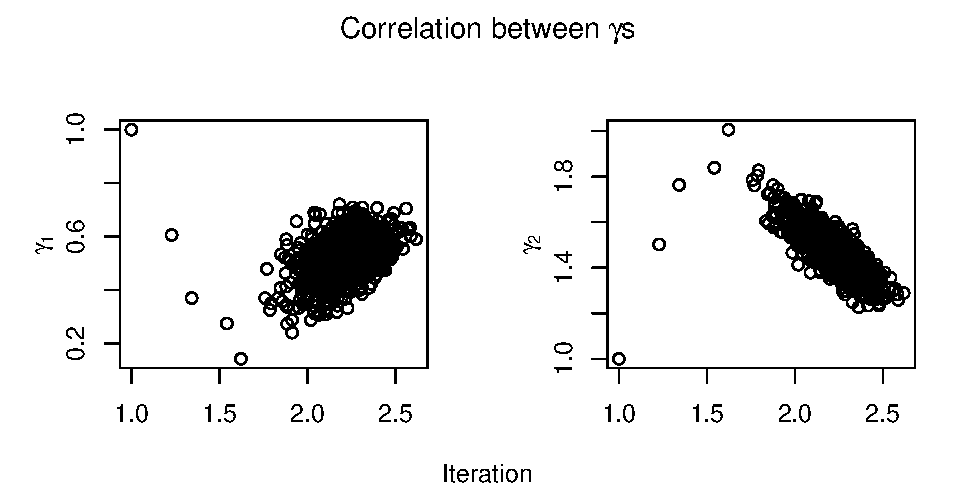
\includegraphics{thesis_draft_files/figure-latex/unnamed-chunk-3-1.pdf}
\caption{\label{fig:migration} Histogram and trace of posterior samples
of the migration rate. This shows relatively slow mixing. This could be
from a combination of the inherent difficulty of exploring the space as
well as poor tuning of the migration proposal.}
\end{figure}

The individual trace plots in Figure \ref{fig:hist_edges} and Figure
\ref{fig:migration} shows that each chain appears to mix rather slowly.
This could be due to the inherent difficulty in exploring the correlated
migration rate/graph space with the current operators.

\begin{figure}
\centering
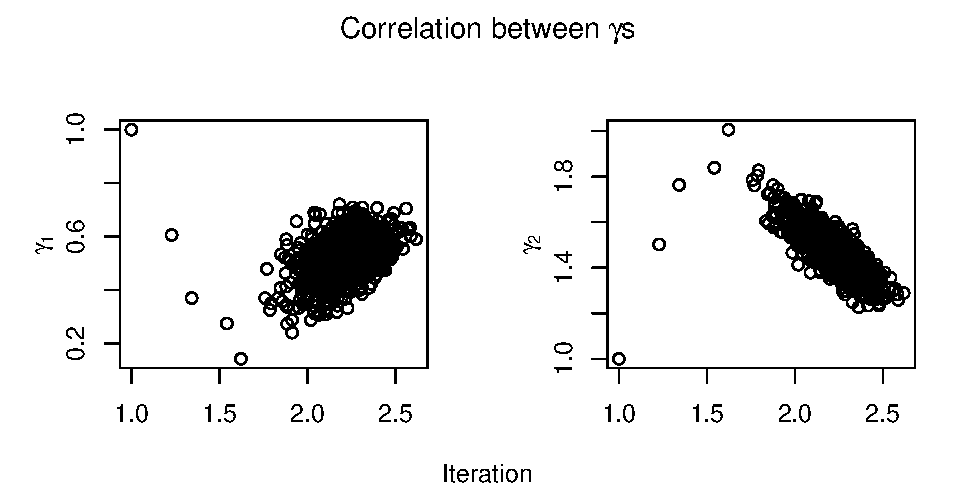
\includegraphics{thesis_draft_files/figure-latex/unnamed-chunk-4-1.pdf}
\caption{\label{fig:pooled} Histograms of pooled samples.}
\end{figure}

\begin{figure}

{\centering 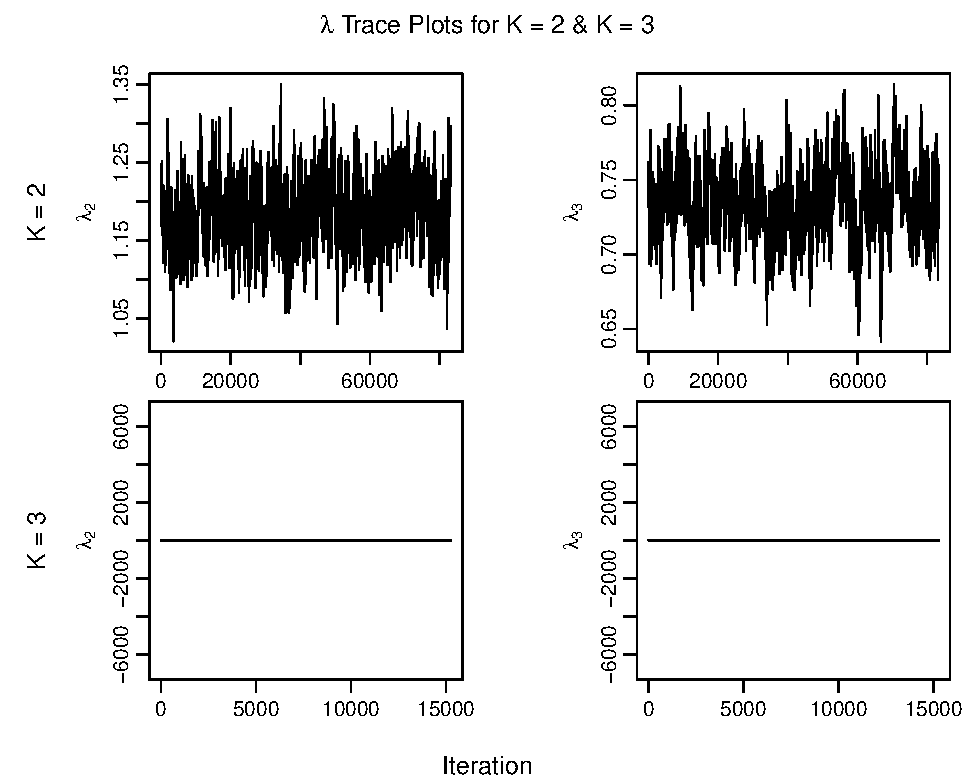
\includegraphics[width=0.65\linewidth]{thesis_draft_files/figure-latex/unnamed-chunk-5-1} 

}

\caption{\label{fig:p_mig_pairs} Joint posterior hex plot between migration rate and $p$ the parameter for the Erdos-Renyi graph. The $p$ value is directly computed from the number of edges by dividing by the total possible edges which is 105. The plot shows a strong negative correlation between $p$ and the migration rate.}\label{fig:unnamed-chunk-5}
\end{figure}

After diagnostics, samples from each of the chains were pooled together.
The effective sample size for the pooled chains are \texttt{11759} and
\texttt{6667} for the number of edges and the migration rate
respectively. Figure \ref{fig:pooled} shows histograms of the pooled
posterior samples of the number of edges and the migration rate. The
mean of the distribution of the number of edges is 16.31 edges and
median is 16 edges. The mean and median are close to the true number of
edges in the graph, \(16\). The mean migration rate is 0.155 and the
median migration rate is 0.151.

Figure \ref{fig:p_mig_pairs} shows a hex plot of the joint posterior
samples of \(p\) (which is computed by \(\frac{\text{num. edges}}{105}\)
where 105 is the maximum number of edges in a graph with 15 vertices)
and migration rate. It shows a strong negative correlation, which is
expected. If the migration rate is smaller than the true value \(m\)
(say \(0.5m\)) then the a city connected to \(d\) cities would need to
connect to \(2d\) many cities to have the ``correct'' counts. Similarly
if the migration rate is higher than the true migration, then the number
of edges would need to be lower than the true number of edges.

The 90\% HPDI for the number of edges and the migration rate are (9, 24)
and (0.08, 0.24) respectively and cover the true values.

\begin{longtable}[]{@{}ccc@{}}
\toprule
parameters & lower & upper\tabularnewline
\midrule
\endhead
\# of edges & 9 & 24\tabularnewline
migration & 0.08 & 0.24\tabularnewline
\bottomrule
\end{longtable}

\pagebreak

\hypertarget{conclusion}{%
\section{Conclusion}\label{conclusion}}

In this thesis, I've re-implemented a Metropolis-Hastings version Held
et al. (\protect\hyperlink{ref-held_two-component_2006}{2006})'s
two-component model and tested the model on simulated data. The MH
version was able to recover the true parameters, with the 90\% HPDI
covering the true parameters. I then extended the model to allow for
multiple time series and a graph informed dependency structure which was
implemented as an adjacency list. To perform inference on the graph,
several graph operators were implemented and tested. Special attention
was payed to computational efficiency of the operators and the
likelihood computation in order to allow the model to scale to larger,
more realistic data sets like the Germany \emph{E. coli} dataset which
contains data from \textasciitilde{} 400 districts each with
\textasciitilde{} 600 time points each.

\hypertarget{data-analysis-of-real-data}{%
\subsection{Data Analysis of Real
Data}\label{data-analysis-of-real-data}}

While the two-component parameters were held fixed to make test the
graph extension, this strategy could also work on a real data set. The
multiple time series can be compressed down to a univariate time series
by summing the data across each city at a particular time step. Then the
two-component parameters can be estimated on this compressed time
series. Then holding these parameters fixed, we could estimate the graph
on the full, uncompressed data. This should give identifical estimates
for the endemic \(\gamma\) parameters, the change points \(K\) and the
location of the change points \(\vec{\theta}\) since these are
independent of the connections between cities. Then only the \(\lambda\)
epidemic parameters need to estimated simulataneously with the graph and
migration rates. This would greatly simplify inference compared with
estimating all the parameters at once.

\hypertarget{future-extension}{%
\subsection{Future Extension}\label{future-extension}}

While this thesis only covers a constant migration rate, the end goal
would be to model the city (vertex) specific and between city (edge)
attributes that could affect the migration rate. For example the size of
the cities (city specific) and the distance between cities (between city
attribute) could be important predictors of migration rates. In the case
of the 2011 outbreak of \emph{E. coli} distance to the Autobahn and
shipping routes might be important since the \emph{E. coli} was carried
on contaminated produce. Determining what factors are most important in
determining migration rates could give clues to e.g., public health
officials, what locations are susceptible to outbreaks and importantly,
what are potential interventions to reduce outbreaks.

The migration rate \(m\) could be modelled as a logistic function of
these city parameters
\(m \sim logit(\beta_0 + \beta_1*X_1 + \beta_2*X_2 + \dots)\) where the
\(X_i\)'s can be both city specific attributes or edge specific
attributes. One simple example could be
\[m_{i,j} \sim \text{logit}\big(\text{pop. city }i*X_1 + \text{pop. city } j*X_2 + \frac{\text{pop. city }i*\text{pop. city }j}{d(\text{city }i, \text{city }j)}*X_3\big), \]
where \(d(i,j)\) is some distance metric (e.g.~euclidean, public
transportation distance). The populations of city \(i\) and city \(j\)
are city specific and
\(\frac{\text{pop. city }i*\text{pop. city }j}{d(\text{city }i, \text{city }j)}\)
is an edge specfic attribute. Then \(m_{ij}\) would be the migration
rate from city \(i\) to city \(j\) and \(m_{j,i}\) the rate from city
\(j\) to city \(i\).

Furthermore this would allow the graph to be changed from an undirected,
unweighted graph to a fully-connected directed graph with weighted
edges, where the weight of \(e_{i,j}\) is \(m_{i,j}\). If the number of
change points \(K\) and the location of the change points
\(\vec{\theta}\) is held fixed (e.g., by being previously estimated),
then all the parameters in the model are continuous and computational
issues regarding the discrete nature of the undirected graph can be
side-stepped. For example, having all the parameters be continuous could
allow for gradient-based sampling methods such as Hamitonian Monte Carlo
which holds the promise of efficient sampling with little to no tuning
required.

\pagebreak

\hypertarget{appendixcode}{%
\section{Appendix/Code}\label{appendixcode}}

\begin{Shaded}
\begin{Highlighting}[]
\NormalTok{pkgs =}\StringTok{ }\KeywordTok{c}\NormalTok{(}\StringTok{"compiler"}\NormalTok{, }\StringTok{"profvis"}\NormalTok{, }\StringTok{"igraph"}\NormalTok{,}\StringTok{"microbenchmark"}\NormalTok{, }\StringTok{"Rcpp"}\NormalTok{)}
\NormalTok{inst =}\StringTok{ }\KeywordTok{lapply}\NormalTok{(pkgs, library, }\DataTypeTok{character.only =} \OtherTok{TRUE}\NormalTok{)}
\end{Highlighting}
\end{Shaded}

\begin{Shaded}
\begin{Highlighting}[]
\CommentTok{#rcpp functions used to speed up parts of the likelihood computation}

\CommentTok{#cpp version of an unnormalized dpois where log = TRUE}
\CommentTok{#pre: two numeric vectors of the same length}
\CommentTok{#post: unnormalized loglikelhood}

\KeywordTok{cppFunction}\NormalTok{(}\StringTok{"double mypois(NumericVector data, NumericVector lambdas) \{}
\StringTok{  int n = data.size();}
\StringTok{  NumericVector plik(n);}
\StringTok{  plik = -lambdas + data*log(lambdas);}

\StringTok{  double tlik = 0;}

\StringTok{  for(int i = 0; i < n; ++i)\{}
\StringTok{    tlik += plik[i];}
\StringTok{  \}}

\StringTok{  return tlik;}
\StringTok{  \}"}\NormalTok{)}

\KeywordTok{cppFunction}\NormalTok{(}\StringTok{"NumericVector diff(NumericVector x)\{}
\StringTok{   return diff(x);}
\StringTok{\}"}\NormalTok{)}

\KeywordTok{cppFunction}\NormalTok{(}\StringTok{"NumericVector sort(NumericVector x) \{}
\StringTok{   NumericVector y = clone(x);}
\StringTok{   std::sort(y.begin(), y.end());}
\StringTok{   return y;}
\StringTok{\}"}\NormalTok{)}
\end{Highlighting}
\end{Shaded}

\begin{Shaded}
\begin{Highlighting}[]
\CommentTok{#cpp version of an unnormalized dpois where log = TRUE}
\CommentTok{#pre: data vector of counts, lambdas a vector of lambda values with }
\CommentTok{# length equal to the number of time points}
\CommentTok{#post: unnormalized loglikelhood}
\NormalTok{mypois <-}\StringTok{ }\ControlFlowTok{function}\NormalTok{(data, lambdas) \{}
  \KeywordTok{sum}\NormalTok{(}\OperatorTok{-}\NormalTok{lambdas }\OperatorTok{+}\StringTok{ }\NormalTok{data}\OperatorTok{*}\KeywordTok{log}\NormalTok{(lambdas))}
\NormalTok{\}}
\end{Highlighting}
\end{Shaded}

\hypertarget{data-simulation}{%
\subsection{Data Simulation}\label{data-simulation}}

\begin{Shaded}
\begin{Highlighting}[]
\CommentTok{#this code block simulates data used in the MCMC}
\CommentTok{#-----------graph initialization-------#}

\CommentTok{# edgelist for handrawn graph}
\NormalTok{el =}\StringTok{ }\KeywordTok{matrix}\NormalTok{(}\KeywordTok{c}\NormalTok{(}\DecValTok{1}\NormalTok{, }\DecValTok{2}\NormalTok{,}
              \DecValTok{1}\NormalTok{, }\DecValTok{3}\NormalTok{,}
              \DecValTok{1}\NormalTok{, }\DecValTok{4}\NormalTok{,}
              \DecValTok{1}\NormalTok{, }\DecValTok{5}\NormalTok{,}
              \DecValTok{1}\NormalTok{, }\DecValTok{6}\NormalTok{,}
              \DecValTok{2}\NormalTok{, }\DecValTok{7}\NormalTok{,}
              \DecValTok{2}\NormalTok{, }\DecValTok{8}\NormalTok{,}
              \DecValTok{7}\NormalTok{, }\DecValTok{8}\NormalTok{,}
              \DecValTok{6}\NormalTok{, }\DecValTok{9}\NormalTok{,}
              \DecValTok{9}\NormalTok{, }\DecValTok{10}\NormalTok{),}
            \DataTypeTok{byrow =} \OtherTok{TRUE}\NormalTok{,}
            \DataTypeTok{ncol =} \DecValTok{2}\NormalTok{)}

\NormalTok{g_city =}\StringTok{ }\KeywordTok{graph_from_edgelist}\NormalTok{(el, }\DataTypeTok{directed =} \OtherTok{FALSE}\NormalTok{)}
\CommentTok{############################################}

\CommentTok{#helpers}
\CommentTok{#unclass from igraph for later use}
\NormalTok{unclass_adjlist <-}\StringTok{ }\ControlFlowTok{function}\NormalTok{(adjlist) \{}
\NormalTok{  adjlist <-}\StringTok{ }\KeywordTok{unclass}\NormalTok{(adjlist)}
  \ControlFlowTok{for}\NormalTok{ (i }\ControlFlowTok{in} \DecValTok{1}\OperatorTok{:}\KeywordTok{length}\NormalTok{(adjlist)) \{}
\NormalTok{    adjlist[[i]] =}\StringTok{ }\KeywordTok{unclass}\NormalTok{(adjlist[[i]])}
\NormalTok{  \}}
  \KeywordTok{return}\NormalTok{(adjlist)}
\NormalTok{\}}

\CommentTok{# ER random graph generation}
\CommentTok{# g_city = sample_gnp(15, 0.175)}
\CommentTok{# plot(g_city)}

\NormalTok{adjlist =}\StringTok{ }\KeywordTok{as_adj_list}\NormalTok{(g_city, }\DataTypeTok{mode =} \StringTok{'all'}\NormalTok{)}
\NormalTok{adjlist <-}\StringTok{ }\KeywordTok{unclass_adjlist}\NormalTok{(adjlist)}

\CommentTok{#---simulate endemic component based on paper's values----#}
\NormalTok{N =}\StringTok{ }\DecValTok{199}     \CommentTok{#total epochs/time steps}
\NormalTok{init =}\StringTok{ }\DecValTok{10}   \CommentTok{#Z_0 value is the initial number of people infected}

\CommentTok{#------- setting endemic parameters-----------------------#}
\NormalTok{gamma  <-}\StringTok{ }\KeywordTok{c}\NormalTok{(}\KeywordTok{log}\NormalTok{(}\DecValTok{10}\NormalTok{), }\FloatTok{0.5}\NormalTok{, }\FloatTok{1.5}\NormalTok{) }\OperatorTok{/}\StringTok{ }\DecValTok{2}
\NormalTok{rho <-}\StringTok{ }\DecValTok{2} \OperatorTok{*}\StringTok{ }\NormalTok{pi }\OperatorTok{/}\StringTok{ }\DecValTok{52}
\NormalTok{t =}\StringTok{ }\DecValTok{1}\OperatorTok{:}\NormalTok{N}
\NormalTok{INDEP <-}
\StringTok{  }\KeywordTok{as.matrix}\NormalTok{(}\KeywordTok{data.frame}\NormalTok{(}
    \DataTypeTok{x0 =} \DecValTok{1}\NormalTok{,}
    \DataTypeTok{x1 =} \KeywordTok{sin}\NormalTok{(rho }\OperatorTok{*}\StringTok{ }\NormalTok{t),}
    \DataTypeTok{x2 =} \KeywordTok{cos}\NormalTok{(rho }\OperatorTok{*}\StringTok{ }\NormalTok{t }\OperatorTok{*}\StringTok{ }\FloatTok{1.5}\NormalTok{)}
\NormalTok{  ))}
\NormalTok{nu_t <-}\StringTok{ }\KeywordTok{as.matrix}\NormalTok{(INDEP) }\OperatorTok\StringTok{ }\NormalTok{gamma}
\NormalTok{ende_lambda =}\StringTok{ }\KeywordTok{rep}\NormalTok{(}\DecValTok{0}\NormalTok{, N)}
\NormalTok{ende_lambda =}\StringTok{ }\KeywordTok{exp}\NormalTok{(nu_t)}

\CommentTok{#-----setting epidemic lambda values -----------}
\NormalTok{K <-}\StringTok{ }\DecValTok{2}              \CommentTok{#changepoints}
\NormalTok{theta  <-}\StringTok{ }\KeywordTok{c}\NormalTok{(}\DecValTok{39}\NormalTok{, }\DecValTok{49}\NormalTok{) }\CommentTok{#location of changepoints}
\NormalTok{migration <-}\StringTok{ }\FloatTok{0.15}

\NormalTok{lambda <-}\StringTok{ }\KeywordTok{c}\NormalTok{(}\FloatTok{0.5}\NormalTok{, }\FloatTok{1.5}\NormalTok{, }\FloatTok{0.5}\NormalTok{) }\OperatorTok{/}\StringTok{ }\DecValTok{2}   \CommentTok{#lambda values}
\NormalTok{epi_lambda =}\StringTok{ }\KeywordTok{rep}\NormalTok{(lambda, }\KeywordTok{diff}\NormalTok{(}\KeywordTok{c}\NormalTok{(}\DecValTok{0}\NormalTok{, theta, N))) }\CommentTok{#lambda vector}

\CommentTok{#-----------------counts matrix ---------#}
\CommentTok{#separate counts from the ende and epi components}
\NormalTok{ende_c =}\StringTok{ }\KeywordTok{matrix}\NormalTok{(}\DecValTok{0}\NormalTok{, }\DataTypeTok{nrow =} \KeywordTok{gorder}\NormalTok{(g_city), }\DataTypeTok{ncol =}\NormalTok{ N)}
\NormalTok{epi_c =}\StringTok{ }\KeywordTok{matrix}\NormalTok{(}\DecValTok{0}\NormalTok{, }\DataTypeTok{nrow =} \KeywordTok{gorder}\NormalTok{(g_city), }\DataTypeTok{ncol =}\NormalTok{ N)}

\NormalTok{counts =}\StringTok{ }\KeywordTok{matrix}\NormalTok{(}\DecValTok{0}\NormalTok{, }\DataTypeTok{nrow =} \KeywordTok{gorder}\NormalTok{(g_city), }\DataTypeTok{ncol =}\NormalTok{ N)}
\NormalTok{counts[, }\DecValTok{1}\NormalTok{] =}\StringTok{ }\NormalTok{init}



\CommentTok{#get list of all adjacent vertices}
\NormalTok{adj =}\StringTok{ }\KeywordTok{as_adj_list}\NormalTok{(g_city)}

\CommentTok{#-----------compute data-----------------#}

\ControlFlowTok{for}\NormalTok{ (i }\ControlFlowTok{in} \DecValTok{1}\OperatorTok{:}\NormalTok{(N }\OperatorTok{-}\StringTok{ }\DecValTok{1}\NormalTok{)) \{}
  \CommentTok{#all rows/cities get same value from the ende}
\NormalTok{  ende_c[, i] =}\StringTok{ }\KeywordTok{rpois}\NormalTok{(}\KeywordTok{gorder}\NormalTok{(g_city), ende_lambda[i])}
  
  \ControlFlowTok{for}\NormalTok{ (j }\ControlFlowTok{in} \DecValTok{1}\OperatorTok{:}\KeywordTok{gorder}\NormalTok{(g_city)) \{}
\NormalTok{    counts_j =}\StringTok{ }\KeywordTok{sum}\NormalTok{(counts[adj[[j]], i]) }\OperatorTok{*}\StringTok{ }\NormalTok{migration }
    \CommentTok{#sum all adjacent counts}
\NormalTok{    counts_j =}\StringTok{ }\NormalTok{counts_j }\OperatorTok{+}\StringTok{ }\NormalTok{counts[j, i] }
    \CommentTok{#add self count}
\NormalTok{    epi_c[j, i] =}\StringTok{ }\KeywordTok{rpois}\NormalTok{(}\DecValTok{1}\NormalTok{, epi_lambda[i] }\OperatorTok{*}\StringTok{ }\NormalTok{counts_j) }
    \CommentTok{#generate new counts}
\NormalTok{    counts[j , i }\OperatorTok{+}\StringTok{ }\DecValTok{1}\NormalTok{] =}\StringTok{ }\NormalTok{ende_c[j, i] }\OperatorTok{+}\StringTok{ }\NormalTok{epi_c[j, i] }
    \CommentTok{#append new counts}
\NormalTok{  \}}
\NormalTok{\}}
\CommentTok{###########################################}
\CommentTok{#list of actual parameter values; useful for testing}

\NormalTok{actual <-}\StringTok{ }\KeywordTok{list}\NormalTok{(}
  \DataTypeTok{K =}\NormalTok{ K,}
  \DataTypeTok{theta =}\NormalTok{ theta,}
  \DataTypeTok{lambda =}\NormalTok{ lambda,}
  \DataTypeTok{LL =} \OperatorTok{-}\OtherTok{Inf}\NormalTok{,}
  \DataTypeTok{gamma =}\NormalTok{ gamma,}
  \DataTypeTok{INDEP =}\NormalTok{ INDEP,}
  \DataTypeTok{graph =}\NormalTok{ g_city,}
  \DataTypeTok{adj =}\NormalTok{ adjlist,}
  \DataTypeTok{counts =}\NormalTok{ counts,}
  \DataTypeTok{migration =}\NormalTok{ migration}
\NormalTok{)}
\end{Highlighting}
\end{Shaded}

\hypertarget{compute_log_prior}{%
\subsection{\texorpdfstring{\texttt{compute\_log\_prior()}}{compute\_log\_prior()}}\label{compute_log_prior}}

\begin{Shaded}
\begin{Highlighting}[]
\CommentTok{#' Computes and returns the log prior of the parameters}
\CommentTok{#'}
\CommentTok{#' @param input a list containing the parameters}
\CommentTok{#' @return the log prior probability of the parameters}

\NormalTok{compute_log_prior <-}\StringTok{ }\ControlFlowTok{function}\NormalTok{(input)\{}
\NormalTok{  K =}\StringTok{ }\NormalTok{input}\OperatorTok{$}\NormalTok{K}
\NormalTok{  theta =}\StringTok{ }\NormalTok{input}\OperatorTok{$}\NormalTok{theta}
\NormalTok{  lambda =}\StringTok{ }\NormalTok{input}\OperatorTok{$}\NormalTok{lambda}
\NormalTok{  gamma =}\StringTok{ }\NormalTok{input}\OperatorTok{$}\NormalTok{gamma}
  
\NormalTok{  adj =}\StringTok{ }\NormalTok{input}\OperatorTok{$}\NormalTok{adj}
\NormalTok{  edge_count =}\StringTok{ }\NormalTok{input}\OperatorTok{$}\NormalTok{edge_count}
  
\NormalTok{  prior_star <-}\StringTok{ }\OperatorTok{-}\KeywordTok{log}\NormalTok{( }\KeywordTok{choose}\NormalTok{( }\KeywordTok{choose}\NormalTok{(}\KeywordTok{length}\NormalTok{(adj), }\DecValTok{2}\NormalTok{), edge_count)) }
   \OperatorTok{-}\KeywordTok{log}\NormalTok{(}\KeywordTok{choose}\NormalTok{(N, K)) }\OperatorTok{+}
\StringTok{     }\KeywordTok{sum}\NormalTok{(}\KeywordTok{dgamma}\NormalTok{(lambda, }\DecValTok{1}\NormalTok{, }\DecValTok{1}\NormalTok{, }\DataTypeTok{log =} \OtherTok{TRUE}\NormalTok{)) }\OperatorTok{+}
\StringTok{     }\KeywordTok{sum}\NormalTok{(}\KeywordTok{dnorm}\NormalTok{(gamma, }\DecValTok{0}\NormalTok{, }\DecValTok{3}\NormalTok{, }\DataTypeTok{log =} \OtherTok{TRUE}\NormalTok{)) }\OperatorTok{+}
\StringTok{     }\KeywordTok{dpois}\NormalTok{(K, }\DecValTok{2}\NormalTok{, }\DataTypeTok{log =} \OtherTok{TRUE}\NormalTok{)}

  \KeywordTok{return}\NormalTok{(prior_star)}
\NormalTok{\}}
\end{Highlighting}
\end{Shaded}

\hypertarget{likelihood-function}{%
\subsection{Likelihood Function}\label{likelihood-function}}

\hypertarget{compute_log_like_diff}{%
\subsubsection{\texorpdfstring{\texttt{compute\_log\_like\_diff()}}{compute\_log\_like\_diff()}}\label{compute_log_like_diff}}

\begin{Shaded}
\begin{Highlighting}[]
\CommentTok{#' Computes the differences in the log-likelihoods between the new graph}
\CommentTok{#' and the old graph and return the difference}
\CommentTok{#' @param input a list containing the parameters}
\CommentTok{#'  (including the proposed adjancency list)}
\CommentTok{#' the old adjacency list and the two vertices that are changed}
\CommentTok{#' @return the log prior probability of the parameters}

\NormalTok{compute_log_like_diff <-}\StringTok{ }\ControlFlowTok{function}\NormalTok{(input, old_adj, v1, v2) \{}
\NormalTok{  K =}\StringTok{ }\NormalTok{input}\OperatorTok{$}\NormalTok{K}
\NormalTok{  theta =}\StringTok{ }\NormalTok{input}\OperatorTok{$}\NormalTok{theta}
\NormalTok{  lambda =}\StringTok{ }\NormalTok{input}\OperatorTok{$}\NormalTok{lambda}
\NormalTok{  gamma =}\StringTok{ }\NormalTok{input}\OperatorTok{$}\NormalTok{gamma}
\NormalTok{  INDEP =}\StringTok{ }\NormalTok{input}\OperatorTok{$}\NormalTok{INDEP}
\NormalTok{  LL =}\StringTok{ }\NormalTok{input}\OperatorTok{$}\NormalTok{LL}
\NormalTok{  adj =}\StringTok{ }\NormalTok{input}\OperatorTok{$}\NormalTok{adj}
\NormalTok{  counts =}\StringTok{ }\NormalTok{input}\OperatorTok{$}\NormalTok{counts}
\NormalTok{  migration =}\StringTok{ }\NormalTok{input}\OperatorTok{$}\NormalTok{migration}
  
  \CommentTok{#replicate lambda values to the }
  \CommentTok{#correct length according to the changepoints}
  \ControlFlowTok{if}\NormalTok{ (K }\OperatorTok{==}\StringTok{ }\DecValTok{0}\NormalTok{) \{}
\NormalTok{    vepi_star <-}\StringTok{ }\KeywordTok{rep}\NormalTok{(lambda, N)}
\NormalTok{  \} }\ControlFlowTok{else}\NormalTok{ \{}
\NormalTok{    vepi_star <-}\StringTok{ }\KeywordTok{rep}\NormalTok{(lambda, }\KeywordTok{diff}\NormalTok{(}\KeywordTok{c}\NormalTok{(}\DecValTok{0}\NormalTok{, theta, N)))}
\NormalTok{  \}}
  
  \CommentTok{#generate the infection counts matrix according to which }
  \CommentTok{# vertices/cities are adjacent}
  
  
  \CommentTok{#---------------new data------------------------------#}
\NormalTok{  inf_counts =}\StringTok{ }\KeywordTok{matrix}\NormalTok{(}\DecValTok{0}\NormalTok{, }\DataTypeTok{nrow =} \DecValTok{2}\NormalTok{, }\DataTypeTok{ncol =}\NormalTok{ N)}
  
\NormalTok{  inf_counts[}\DecValTok{1}\NormalTok{, ] =}\StringTok{ }\KeywordTok{.colSums}\NormalTok{(counts[adj[[v1]], , }\DataTypeTok{drop =} \OtherTok{FALSE}\NormalTok{],}
                             \KeywordTok{length}\NormalTok{(adj[[v1]]), N) }\OperatorTok{*}
\StringTok{    }\NormalTok{migration }\OperatorTok{+}\StringTok{ }\NormalTok{counts[v1, ]}
  
\NormalTok{  inf_counts[}\DecValTok{2}\NormalTok{, ] =}\StringTok{ }\KeywordTok{.colSums}\NormalTok{(counts[adj[[v2]], , }\DataTypeTok{drop =} \OtherTok{FALSE}\NormalTok{],}
                             
                             \KeywordTok{length}\NormalTok{(adj[[v2]]), N) }\OperatorTok{*}
\StringTok{    }\NormalTok{migration }\OperatorTok{+}\StringTok{ }\NormalTok{counts[v2, ]}
  
  \CommentTok{#######################################################}
  
  \CommentTok{#------------------old data------------------------------#}
  
\NormalTok{  old_inf_counts =}\StringTok{ }\KeywordTok{matrix}\NormalTok{(}\DecValTok{0}\NormalTok{, }\DataTypeTok{nrow =} \DecValTok{2}\NormalTok{, }\DataTypeTok{ncol =}\NormalTok{ N)}
  
\NormalTok{  old_inf_counts[}\DecValTok{1}\NormalTok{, ] =}\StringTok{ }\KeywordTok{.colSums}\NormalTok{(counts[old_adj[[v1]], , }\DataTypeTok{drop =} \OtherTok{FALSE}\NormalTok{]}
\NormalTok{                                 , }\KeywordTok{length}\NormalTok{(old_adj[[v1]]), N) }\OperatorTok{*}
\StringTok{    }\NormalTok{migration }\OperatorTok{+}\StringTok{ }\NormalTok{counts[v1,]}
  
\NormalTok{  old_inf_counts[}\DecValTok{2}\NormalTok{, ] =}\StringTok{ }\KeywordTok{.colSums}\NormalTok{(counts[old_adj[[v2]], , }\DataTypeTok{drop =} \OtherTok{FALSE}\NormalTok{]}
\NormalTok{                                 , }\KeywordTok{length}\NormalTok{(old_adj[[v2]]), N) }\OperatorTok{*}
\StringTok{    }\NormalTok{migration }\OperatorTok{+}\StringTok{ }\NormalTok{counts[v2, ]}
  \CommentTok{#######################################################}
  
  
  \CommentTok{# ------- endemic and epidemic parameter matrices -----}
\NormalTok{  nu <-}\StringTok{ }\KeywordTok{exp}\NormalTok{(INDEP }\OperatorTok\StringTok{ }\NormalTok{gamma)  }\CommentTok{#generate nu parameter for endemic}
\NormalTok{  mat_ende_lambda <-}\StringTok{ }\KeywordTok{matrix}\NormalTok{(}\KeywordTok{rep}\NormalTok{(nu, }\DecValTok{2}\NormalTok{), }\DataTypeTok{nrow =} \DecValTok{2}\NormalTok{, }\DataTypeTok{byrow =} \OtherTok{TRUE}\NormalTok{)}
  
  \CommentTok{#creates matrix of lambdas from estimated lambda row}
\NormalTok{  mat_lambdas <-}
\StringTok{    }\KeywordTok{matrix}\NormalTok{(}\KeywordTok{rep}\NormalTok{(vepi_star, }\DecValTok{2}\NormalTok{), }\DataTypeTok{nrow =} \DecValTok{2}\NormalTok{, }\DataTypeTok{byrow =} \OtherTok{TRUE}\NormalTok{)}
  \CommentTok{#######################################################}
  
  \CommentTok{#-----------compute the log-likelihoods---------------#}
  \CommentTok{#data is for 2:N, first column is an initial value}
\NormalTok{  new_log_lik <-}
\StringTok{    }\KeywordTok{mypois}\NormalTok{(counts[}\KeywordTok{c}\NormalTok{(v1, v2), }\DecValTok{2}\OperatorTok{:}\NormalTok{N],}
\NormalTok{           inf_counts[, }\DecValTok{1}\OperatorTok{:}\NormalTok{(N }\OperatorTok{-}\StringTok{ }\DecValTok{1}\NormalTok{)] }\OperatorTok{*}\StringTok{ }\NormalTok{mat_lambdas[, }\DecValTok{1}\OperatorTok{:}\NormalTok{(N }\OperatorTok{-}\StringTok{ }\DecValTok{1}\NormalTok{)]}
           \OperatorTok{+}\StringTok{ }\NormalTok{mat_ende_lambda[, }\DecValTok{1}\OperatorTok{:}\NormalTok{(N }\OperatorTok{-}\StringTok{ }\DecValTok{1}\NormalTok{)])}
  
\NormalTok{  old_log_lik <-}
\StringTok{    }\KeywordTok{mypois}\NormalTok{(counts[}\KeywordTok{c}\NormalTok{(v1, v2), }\DecValTok{2}\OperatorTok{:}\NormalTok{N],}
\NormalTok{           old_inf_counts[, }\DecValTok{1}\OperatorTok{:}\NormalTok{(N }\OperatorTok{-}\StringTok{ }\DecValTok{1}\NormalTok{)] }\OperatorTok{*}\StringTok{ }\NormalTok{mat_lambdas[, }\DecValTok{1}\OperatorTok{:}\NormalTok{(N }\OperatorTok{-}\StringTok{ }\DecValTok{1}\NormalTok{)]}
           \OperatorTok{+}\StringTok{ }\NormalTok{mat_ende_lambda[, }\DecValTok{1}\OperatorTok{:}\NormalTok{(N }\OperatorTok{-}\StringTok{ }\DecValTok{1}\NormalTok{)])}
  \CommentTok{##################################################S#####}
  
  \KeywordTok{return}\NormalTok{(new_log_lik }\OperatorTok{-}\StringTok{ }\NormalTok{old_log_lik)}
\NormalTok{\}}
\end{Highlighting}
\end{Shaded}

\hypertarget{compute_log_like}{%
\subsubsection{\texorpdfstring{\texttt{compute\_log\_like()}}{compute\_log\_like()}}\label{compute_log_like}}

\begin{Shaded}
\begin{Highlighting}[]
\CommentTok{#' Computes and returns the unnormalized graph }
\CommentTok{#' log likelihood of the parameters. Recomputes all the data.}
\CommentTok{#' @param input a list containing the parameters}
\CommentTok{#' @return the log likelihood probability of the parameters}

\NormalTok{compute_log_like <-}\StringTok{ }\ControlFlowTok{function}\NormalTok{(input) \{}
\NormalTok{  K =}\StringTok{ }\NormalTok{input}\OperatorTok{$}\NormalTok{K}
\NormalTok{  theta =}\StringTok{ }\NormalTok{input}\OperatorTok{$}\NormalTok{theta}
\NormalTok{  lambda =}\StringTok{ }\NormalTok{input}\OperatorTok{$}\NormalTok{lambda}
\NormalTok{  gamma =}\StringTok{ }\NormalTok{input}\OperatorTok{$}\NormalTok{gamma}
\NormalTok{  INDEP =}\StringTok{ }\NormalTok{input}\OperatorTok{$}\NormalTok{INDEP}
\NormalTok{  LL =}\StringTok{ }\NormalTok{input}\OperatorTok{$}\NormalTok{LL}
\NormalTok{  adj =}\StringTok{ }\NormalTok{input}\OperatorTok{$}\NormalTok{adj}
\NormalTok{  counts =}\StringTok{ }\NormalTok{input}\OperatorTok{$}\NormalTok{counts}
\NormalTok{  migration =}\StringTok{ }\NormalTok{input}\OperatorTok{$}\NormalTok{migration}
  
  \CommentTok{#replicate lambda values to the correct }
  \CommentTok{#length according to the changepoints}
  \ControlFlowTok{if}\NormalTok{ (K }\OperatorTok{==}\StringTok{ }\DecValTok{0}\NormalTok{) \{}
\NormalTok{    vepi_star <-}\StringTok{ }\KeywordTok{rep}\NormalTok{(lambda, N)}
\NormalTok{  \} }\ControlFlowTok{else}\NormalTok{ \{}
\NormalTok{    vepi_star <-}\StringTok{ }\KeywordTok{rep}\NormalTok{(lambda, }\KeywordTok{diff}\NormalTok{(}\KeywordTok{c}\NormalTok{(}\DecValTok{0}\NormalTok{, theta, N)))}
\NormalTok{  \}}
  
  \CommentTok{#generate the infection counts matrix according to which}
  \CommentTok{# vertices/cities are adjacent}
\NormalTok{  ord =}\StringTok{ }\KeywordTok{length}\NormalTok{(adj)  }\CommentTok{#number of vertices in the graph}
\NormalTok{  inf_counts =}\StringTok{ }\KeywordTok{matrix}\NormalTok{(}\DecValTok{0}\NormalTok{, }\DataTypeTok{nrow =}\NormalTok{ ord, }\DataTypeTok{ncol =}\NormalTok{ N)}
  
  \ControlFlowTok{for}\NormalTok{ (i }\ControlFlowTok{in} \DecValTok{1}\OperatorTok{:}\NormalTok{ord) \{}
    \CommentTok{#inf_counts[i, ] = colSums(counts[adj[[i]], , drop = FALSE])*}
    \CommentTok{#migration + counts[i, ]}
\NormalTok{    inf_counts[i, ] =}\StringTok{ }\KeywordTok{.colSums}\NormalTok{(counts[adj[[i]], , }\DataTypeTok{drop =} \OtherTok{FALSE}\NormalTok{]}
\NormalTok{                      , }\KeywordTok{length}\NormalTok{(adj[[i]]), N)}\OperatorTok{*}\NormalTok{migration }\OperatorTok{+}\StringTok{ }\NormalTok{counts[i, ]}
\NormalTok{  \}}
  
  \CommentTok{# ------- endemic and epidemic parameter matrices ----}
\NormalTok{  nu <-}\StringTok{ }\KeywordTok{exp}\NormalTok{(INDEP }\OperatorTok\StringTok{ }\NormalTok{gamma)         }\CommentTok{#generate nu parameter for endemic}
  \CommentTok{#creates matrix of repeated rows}
\NormalTok{  mat_ende_lambda <-}\StringTok{ }\KeywordTok{matrix}\NormalTok{(}\KeywordTok{rep}\NormalTok{(nu, ord), }\DataTypeTok{nrow =}\NormalTok{ ord, }\DataTypeTok{byrow =} \OtherTok{TRUE}\NormalTok{)}
  
  \CommentTok{#creates matrix of lambdas from estimated lambda row}
\NormalTok{  mat_lambdas <-}
\StringTok{    }\KeywordTok{matrix}\NormalTok{(}\KeywordTok{rep}\NormalTok{(vepi_star, ord), }\DataTypeTok{nrow =}\NormalTok{ ord, }\DataTypeTok{byrow =} \OtherTok{TRUE}\NormalTok{)}
  
  \CommentTok{#compute the log-likelihood}
  \CommentTok{#data is for 2:N, first column is an initial value}
\NormalTok{  log_lik <-}
\StringTok{    }\KeywordTok{mypois}\NormalTok{(counts[, }\DecValTok{2}\OperatorTok{:}\NormalTok{N], }
\NormalTok{           inf_counts[, }\DecValTok{1}\OperatorTok{:}\NormalTok{(N }\OperatorTok{-}\StringTok{ }\DecValTok{1}\NormalTok{)] }\OperatorTok{*}\StringTok{ }\NormalTok{mat_lambdas[, }\DecValTok{1}\OperatorTok{:}\NormalTok{(N }\OperatorTok{-}\StringTok{ }\DecValTok{1}\NormalTok{)] }
           \OperatorTok{+}\StringTok{ }\NormalTok{mat_ende_lambda[, }\DecValTok{1}\OperatorTok{:}\NormalTok{(N }\OperatorTok{-}\StringTok{ }\DecValTok{1}\NormalTok{)])}
  
  \KeywordTok{return}\NormalTok{(log_lik)}
\NormalTok{\}}

\CommentTok{#-------for prior testing--------}

 \CommentTok{# compute_log_like_diff <- function(input, adj, v1,v2)\{}
 \CommentTok{#   0}
 \CommentTok{# \}}
\end{Highlighting}
\end{Shaded}

\hypertarget{non-graph-operators}{%
\subsection{Non-graph Operators}\label{non-graph-operators}}

\hypertarget{change_migration-1}{%
\subsubsection{\texorpdfstring{\texttt{change\_migration()}}{change\_migration()}}\label{change_migration-1}}

\begin{Shaded}
\begin{Highlighting}[]
\CommentTok{#' Proposes a new migration value using a MRW with a uniform }
\CommentTok{#' distribution}
\CommentTok{#' @param input a list containing the parameters}
\CommentTok{#' @return a list of either the newly proposed }
\CommentTok{#' state (input_star) or the state}

\NormalTok{change_migration <-}\StringTok{ }\ControlFlowTok{function}\NormalTok{(input) \{}
\NormalTok{  LL <-}\StringTok{ }\NormalTok{input}\OperatorTok{$}\NormalTok{LL}
\NormalTok{  migration <-}\StringTok{ }\NormalTok{input}\OperatorTok{$}\NormalTok{migration}
  
  \CommentTok{#propose new state from normal}
\NormalTok{  migration_star <-}\StringTok{ }\NormalTok{migration }\OperatorTok{+}\StringTok{ }\KeywordTok{runif}\NormalTok{(}\DecValTok{1}\NormalTok{, }\FloatTok{-0.01}\NormalTok{, }\FloatTok{0.01}\NormalTok{)}
  
  \ControlFlowTok{if}\NormalTok{ (migration_star }\OperatorTok{>}\StringTok{ }\DecValTok{1} \OperatorTok{||}\StringTok{ }\NormalTok{migration_star }\OperatorTok{<}\StringTok{ }\DecValTok{0}\NormalTok{)\{}
    \KeywordTok{return}\NormalTok{(input)}
\NormalTok{  \}}
  
  \CommentTok{#repackage list}
\NormalTok{  input_star <-}\StringTok{ }\NormalTok{input}
\NormalTok{  input_star}\OperatorTok{$}\NormalTok{migration <-}\StringTok{ }\NormalTok{migration_star}
  
\NormalTok{  LL_star <-}\StringTok{ }\KeywordTok{compute_log_like}\NormalTok{(input_star) }\CommentTok{#compute log likelihood}
\NormalTok{  prior_star <-}\StringTok{  }\KeywordTok{compute_log_prior}\NormalTok{(input_star) }\CommentTok{#compute LOG prior}
\NormalTok{  post_star <-}\StringTok{ }\NormalTok{LL_star }\OperatorTok{+}\StringTok{ }\NormalTok{prior_star }\CommentTok{#new log posterior}
  
\NormalTok{  U =}\StringTok{ }\KeywordTok{runif}\NormalTok{(}\DecValTok{1}\NormalTok{)}
  
  \ControlFlowTok{if}\NormalTok{ (}\KeywordTok{log}\NormalTok{(U) }\OperatorTok{<}\StringTok{ }\NormalTok{post_star }\OperatorTok{-}\StringTok{ }\NormalTok{LL) \{}
\NormalTok{    input_star}\OperatorTok{$}\NormalTok{LL <-}\StringTok{ }\NormalTok{post_star}
    \KeywordTok{return}\NormalTok{(input_star)}
\NormalTok{  \} }\ControlFlowTok{else}\NormalTok{ \{}
    \KeywordTok{return}\NormalTok{(input)}
\NormalTok{  \}}
  
\NormalTok{\}}
\end{Highlighting}
\end{Shaded}

\hypertarget{change_gamma-death_theta-birth_theta}{%
\subsubsection{\texorpdfstring{\texttt{change\_gamma()},
\texttt{death\_theta()},
\texttt{birth\_theta()}}{change\_gamma(), death\_theta(), birth\_theta()}}\label{change_gamma-death_theta-birth_theta}}

\begin{Shaded}
\begin{Highlighting}[]
\CommentTok{#' Proposes a new gamma parameter vector from a random normal}
\CommentTok{#'  Metropolis Random Walk (MRW)}
\CommentTok{#' @param input a list containing the current parameter state}
\CommentTok{#' @return a list of either the newly proposed state (input_star) or the}
\CommentTok{#' current Metropolis Random Walk (MRW)}

\NormalTok{change_gamma <-}\StringTok{ }\ControlFlowTok{function}\NormalTok{(input) \{}
\NormalTok{  LL <-}\StringTok{ }\NormalTok{input}\OperatorTok{$}\NormalTok{LL}
\NormalTok{  gamma <-}\StringTok{ }\NormalTok{input}\OperatorTok{$}\NormalTok{gamma}
  
  \CommentTok{#propose new state from normal}
\NormalTok{  gamma_star <-}\StringTok{ }\NormalTok{gamma }\OperatorTok{+}\StringTok{ }\KeywordTok{rnorm}\NormalTok{(}\DecValTok{3}\NormalTok{, }\DecValTok{0}\NormalTok{, }\FloatTok{0.01}\NormalTok{)}
  
  \CommentTok{#repackage list}
\NormalTok{  input_star <-}\StringTok{ }\NormalTok{input}
\NormalTok{  input_star}\OperatorTok{$}\NormalTok{gamma <-}\StringTok{ }\NormalTok{gamma_star}
  
\NormalTok{  LL_star <-}\StringTok{ }\KeywordTok{compute_log_like}\NormalTok{(input_star) }\CommentTok{#compute log likelihood}
\NormalTok{  prior_star <-}\StringTok{  }\KeywordTok{compute_log_prior}\NormalTok{(input_star) }\CommentTok{#compute LOG prior}
\NormalTok{  post_star <-}\StringTok{ }\NormalTok{LL_star }\OperatorTok{+}\StringTok{ }\NormalTok{prior_star }\CommentTok{#new log posterior}
  
\NormalTok{  U =}\StringTok{ }\KeywordTok{runif}\NormalTok{(}\DecValTok{1}\NormalTok{)}
  
  \ControlFlowTok{if}\NormalTok{ (}\KeywordTok{log}\NormalTok{(U) }\OperatorTok{<}\StringTok{ }\NormalTok{post_star }\OperatorTok{-}\StringTok{ }\NormalTok{LL) \{}
\NormalTok{    input_star}\OperatorTok{$}\NormalTok{LL <-}\StringTok{ }\NormalTok{post_star}
    \KeywordTok{return}\NormalTok{(input_star)}
\NormalTok{  \} }\ControlFlowTok{else}\NormalTok{ \{}
    \KeywordTok{return}\NormalTok{(input)}
\NormalTok{  \}}
  
\NormalTok{\}}


\CommentTok{#' Proposes removing a changepoint. Uses a Reversible Jump MCMC (RJMCMC)}
\CommentTok{#'as seen in Green 1995}
\CommentTok{#' @param input a list containing the current parameter state}
\CommentTok{#' @return a list of either the newly proposed state (input_star) or the}
\CommentTok{#' current state (input)}


\NormalTok{death_theta <-}\StringTok{ }\ControlFlowTok{function}\NormalTok{(input) \{}
\NormalTok{  K =}\StringTok{ }\NormalTok{input}\OperatorTok{$}\NormalTok{K}
\NormalTok{  theta =}\StringTok{ }\NormalTok{input}\OperatorTok{$}\NormalTok{theta}
\NormalTok{  lambda =}\StringTok{ }\NormalTok{input}\OperatorTok{$}\NormalTok{lambda}
\NormalTok{  LL =}\StringTok{ }\NormalTok{input}\OperatorTok{$}\NormalTok{LL}
  
  \CommentTok{#if K = 0 (no change points) then automatically reject this proposal}
  \ControlFlowTok{if}\NormalTok{ (K }\OperatorTok{==}\StringTok{ }\DecValTok{0}\NormalTok{) \{}
    \KeywordTok{return}\NormalTok{(input)}
\NormalTok{  \}}
  
  \CommentTok{#randomly sample from the current list of changepoints}
\NormalTok{  m <-}\StringTok{ }\KeywordTok{ceiling}\NormalTok{(}\KeywordTok{runif}\NormalTok{(}\DecValTok{1}\NormalTok{, }\DecValTok{0}\NormalTok{, }\KeywordTok{length}\NormalTok{(theta)))}
\NormalTok{  theta_star <-}\StringTok{ }\NormalTok{theta[}\KeywordTok{c}\NormalTok{(}\OperatorTok{-}\NormalTok{m)]  }\CommentTok{# remove that from the list}
  
  \CommentTok{#adjusting lambda values due to removal of changepoint}
  \CommentTok{#find lambda values that were adjacent to changepoint m}
\NormalTok{  lambda1 <-}\StringTok{ }\NormalTok{lambda[m]}
\NormalTok{  lambda2 <-}\StringTok{ }\NormalTok{lambda[m }\OperatorTok{+}\StringTok{ }\DecValTok{1}\NormalTok{]}
  
  \CommentTok{#adds endpoints to the vector of theta values}
\NormalTok{  temp_theta =}\StringTok{ }\KeywordTok{c}\NormalTok{(}\DecValTok{0}\NormalTok{, theta, N)}
\NormalTok{  j =}\StringTok{ }\NormalTok{m }\OperatorTok{+}\StringTok{ }\DecValTok{1}
  
  \CommentTok{#crate new value as a}
  \CommentTok{#geometric weighted sum of the previous two lambda values}
\NormalTok{  lambda0 <-}
\StringTok{    }\NormalTok{lambda1 }\OperatorTok{^}\StringTok{ }\NormalTok{((temp_theta[j] }\OperatorTok{-}\StringTok{ }\NormalTok{temp_theta[j }\OperatorTok{-}\StringTok{ }\DecValTok{1}\NormalTok{]) }\OperatorTok{/}
\StringTok{                 }\NormalTok{(temp_theta[j }\OperatorTok{+}\StringTok{ }\DecValTok{1}\NormalTok{] }\OperatorTok{-}\StringTok{ }\NormalTok{temp_theta[j }\OperatorTok{-}\StringTok{ }\DecValTok{1}\NormalTok{])) }\OperatorTok{*}
\StringTok{    }\NormalTok{lambda2 }\OperatorTok{^}\StringTok{ }\NormalTok{((temp_theta[j }\OperatorTok{+}\StringTok{ }\DecValTok{1}\NormalTok{] }\OperatorTok{-}\StringTok{ }\NormalTok{temp_theta[j]) }\OperatorTok{/}
\StringTok{                 }\NormalTok{(temp_theta[j }\OperatorTok{+}\StringTok{ }\DecValTok{1}\NormalTok{] }\OperatorTok{-}\StringTok{ }\NormalTok{temp_theta[j }\OperatorTok{-}\StringTok{ }\DecValTok{1}\NormalTok{]))}
  
  \CommentTok{#create new lambda proposal vector}
\NormalTok{  lambda_star <-}\StringTok{ }\NormalTok{lambda}
\NormalTok{  lambda_star[m] <-}
\StringTok{    }\NormalTok{lambda0 }\CommentTok{#insert the lambda value into the correct location}
\NormalTok{  lambda_star <-}\StringTok{ }\NormalTok{lambda_star[}\OperatorTok{-}\KeywordTok{c}\NormalTok{(m }\OperatorTok{+}\StringTok{ }\DecValTok{1}\NormalTok{)] }\CommentTok{#delete the extra value}
  
  \CommentTok{#repackage values into input_star}
\NormalTok{  input_star <-}\StringTok{ }\NormalTok{input}
\NormalTok{  input_star}\OperatorTok{$}\NormalTok{lambda <-}\StringTok{ }\NormalTok{lambda_star}
\NormalTok{  input_star}\OperatorTok{$}\NormalTok{theta <-}\StringTok{ }\NormalTok{theta_star}
\NormalTok{  input_star}\OperatorTok{$}\NormalTok{K <-}\StringTok{ }\NormalTok{K }\OperatorTok{-}\StringTok{ }\DecValTok{1}
  
  \CommentTok{#compute log likelihood}
\NormalTok{  LL_star <-}\StringTok{ }\KeywordTok{compute_log_like}\NormalTok{(input_star)}
  \CommentTok{#compule log prior}
\NormalTok{  prior_star <-}\StringTok{  }\KeywordTok{compute_log_prior}\NormalTok{(input_star)}
\NormalTok{  post_star <-}\StringTok{ }\NormalTok{LL_star }\OperatorTok{+}\StringTok{ }\NormalTok{prior_star }\CommentTok{#new log posterior}
  
  \CommentTok{#hastings ratio}
\NormalTok{  hastings <-}\StringTok{ }\KeywordTok{log}\NormalTok{(K) }\OperatorTok{-}\StringTok{ }\KeywordTok{log}\NormalTok{(N }\OperatorTok{-}\StringTok{ }\NormalTok{(K }\OperatorTok{-}\StringTok{ }\DecValTok{1}\NormalTok{))}
  
  \CommentTok{#value preserving jacobian for RJMCMC}
\NormalTok{  log_jacobian <-}\StringTok{ }\DecValTok{-2} \OperatorTok{*}\StringTok{ }\KeywordTok{log}\NormalTok{(lambda1 }\OperatorTok{+}\StringTok{ }\NormalTok{lambda2) }\OperatorTok{+}\StringTok{ }\KeywordTok{log}\NormalTok{(lambda0)}
  \CommentTok{#final log acceptance}
\NormalTok{  alpha <-}\StringTok{ }\NormalTok{post_star  }\OperatorTok{-}\StringTok{ }\NormalTok{LL }\OperatorTok{+}\StringTok{ }\NormalTok{log_jacobian }\OperatorTok{+}\StringTok{ }\NormalTok{hastings}
  
  \ControlFlowTok{if}\NormalTok{ (alpha }\OperatorTok{>}\StringTok{ }\KeywordTok{log}\NormalTok{(}\KeywordTok{runif}\NormalTok{(}\DecValTok{1}\NormalTok{))) \{}
\NormalTok{    input_star}\OperatorTok{$}\NormalTok{LL <-}\StringTok{ }\NormalTok{post_star}
    \KeywordTok{return}\NormalTok{(input_star)}
\NormalTok{  \}  }\ControlFlowTok{else}\NormalTok{ \{}
    \KeywordTok{return}\NormalTok{(input)}
\NormalTok{  \}}
\NormalTok{\}}


\CommentTok{#' Proposes adding a changepoint. Uses a Reversible Jump MCMC (RJMCMC) }
\CommentTok{#' as seen  in Green 1995}
\CommentTok{#' @param input a list containing the current parameter state}
\CommentTok{#' @return a list of either the newly proposed state (input_star) }
\CommentTok{#' or the current  state (input)}


\NormalTok{birth_theta <-}\StringTok{ }\ControlFlowTok{function}\NormalTok{(input) \{}
\NormalTok{  K =}\StringTok{ }\NormalTok{input}\OperatorTok{$}\NormalTok{K}
\NormalTok{  theta =}\StringTok{ }\NormalTok{input}\OperatorTok{$}\NormalTok{theta}
\NormalTok{  lambda =}\StringTok{ }\NormalTok{input}\OperatorTok{$}\NormalTok{lambda}
  
\NormalTok{  LL =}\StringTok{ }\NormalTok{input}\OperatorTok{$}\NormalTok{LL}
  
  \CommentTok{#if K = N, the max number of time }
  \CommentTok{#steps then automatically reject this propos}
  \ControlFlowTok{if}\NormalTok{ (K }\OperatorTok{==}\StringTok{ }\NormalTok{N) \{}
    \KeywordTok{return}\NormalTok{(input)}
\NormalTok{  \}}
  
  
  \CommentTok{#theta_m <- sample(setdiff(1:N, theta), 1)  # birth}
  
  \CommentTok{#randomly sample from all possible time steps}
\NormalTok{  theta_m <-}\StringTok{ }\KeywordTok{ceiling}\NormalTok{(}\KeywordTok{runif}\NormalTok{(}\DecValTok{1}\NormalTok{, }\DecValTok{0}\NormalTok{, N))}
  \CommentTok{#resample if the time step is already in the changepoint list}
  \ControlFlowTok{while}\NormalTok{ (theta_m }\OperatorTok\StringTok{ }\NormalTok{theta) \{}
\NormalTok{    theta_m <-}\StringTok{ }\KeywordTok{ceiling}\NormalTok{(}\KeywordTok{runif}\NormalTok{(}\DecValTok{1}\NormalTok{, }\DecValTok{0}\NormalTok{, N))}
\NormalTok{  \}}
  
  \CommentTok{#create a theta vector with the newly proposed changepoint}
\NormalTok{  theta_star <-}\StringTok{ }\KeywordTok{sort}\NormalTok{(}\KeywordTok{c}\NormalTok{(theta, theta_m))}
  \CommentTok{#determine the location of the changepoint in the vector}
\NormalTok{  m <-}\StringTok{ }\KeywordTok{which}\NormalTok{(theta_star }\OperatorTok{==}\StringTok{ }\NormalTok{theta_m)}
  
  \CommentTok{#add endpoints}
\NormalTok{  temp_theta_star =}\StringTok{ }\KeywordTok{c}\NormalTok{(}\DecValTok{0}\NormalTok{, theta_star, N)}
  
  \CommentTok{#---update lambda vectors; RJMCMC}
\NormalTok{  u <-}\StringTok{ }\KeywordTok{runif}\NormalTok{(}\DecValTok{1}\NormalTok{)}
\NormalTok{  j =}\StringTok{ }\NormalTok{m }\OperatorTok{+}\StringTok{ }\DecValTok{1} \CommentTok{#indexing help}
  \CommentTok{#take original lambda value and split is as a geoemtric average}
\NormalTok{  lambda0 <-}\StringTok{ }\NormalTok{lambda[m]}
\NormalTok{  lambda1 <-}
\StringTok{    }\NormalTok{lambda0 }\OperatorTok{*}\StringTok{ }\NormalTok{(u }\OperatorTok{/}\StringTok{ }\NormalTok{(}\DecValTok{1} \OperatorTok{-}\StringTok{ }\NormalTok{u)) }\OperatorTok{^}
\StringTok{    }\NormalTok{((temp_theta_star[j] }\OperatorTok{-}\StringTok{ }\NormalTok{temp_theta_star[j }\OperatorTok{-}\StringTok{ }\DecValTok{1}\NormalTok{]) }\OperatorTok{/}
\StringTok{                                 }
\StringTok{    }\NormalTok{(temp_theta_star[j }\OperatorTok{+}\StringTok{ }\DecValTok{1}\NormalTok{] }\OperatorTok{-}\StringTok{ }\NormalTok{temp_theta_star[j }\OperatorTok{-}\StringTok{ }\DecValTok{1}\NormalTok{]))}
  
\NormalTok{  lambda2 <-}
\StringTok{    }\NormalTok{lambda0 }\OperatorTok{*}\StringTok{ }\NormalTok{((}\DecValTok{1} \OperatorTok{-}\StringTok{ }\NormalTok{u) }\OperatorTok{/}\StringTok{ }\NormalTok{u) }\OperatorTok{^}
\StringTok{    }\NormalTok{((temp_theta_star[j }\OperatorTok{+}\StringTok{ }\DecValTok{1}\NormalTok{] }\OperatorTok{-}\StringTok{ }\NormalTok{temp_theta_star[j]) }\OperatorTok{/}
\StringTok{    }\NormalTok{(temp_theta_star[j }\OperatorTok{+}\StringTok{ }\DecValTok{1}\NormalTok{] }\OperatorTok{-}\StringTok{ }\NormalTok{temp_theta_star[j }\OperatorTok{-}\StringTok{ }\DecValTok{1}\NormalTok{]))}
  
  \CommentTok{#edge case when there is no changepoint}
  \ControlFlowTok{if}\NormalTok{ (K }\OperatorTok{==}\StringTok{ }\DecValTok{0}\NormalTok{) \{}
\NormalTok{    lambda0 <-}\StringTok{ }\NormalTok{lambda[}\DecValTok{1}\NormalTok{]}
\NormalTok{    lambda1 <-}
\StringTok{      }\NormalTok{lambda0 }\OperatorTok{*}\StringTok{ }\NormalTok{(u }\OperatorTok{/}\StringTok{ }\NormalTok{(}\DecValTok{1} \OperatorTok{-}\StringTok{ }\NormalTok{u)) }\OperatorTok{^}
\StringTok{      }\NormalTok{((temp_theta_star[j] }\OperatorTok{-}\StringTok{ }\NormalTok{temp_theta_star[j }\OperatorTok{-}\StringTok{ }\DecValTok{1}\NormalTok{]) }\OperatorTok{/}
\StringTok{     }\NormalTok{(temp_theta_star[j }\OperatorTok{+}\StringTok{ }\DecValTok{1}\NormalTok{] }\OperatorTok{-}\StringTok{ }\NormalTok{temp_theta_star[j }\OperatorTok{-}\StringTok{ }\DecValTok{1}\NormalTok{]))}
    
\NormalTok{    lambda2 <-}
\StringTok{      }\NormalTok{lambda0 }\OperatorTok{*}\StringTok{ }\NormalTok{((}\DecValTok{1} \OperatorTok{-}\StringTok{ }\NormalTok{u) }\OperatorTok{/}\StringTok{ }\NormalTok{u) }\OperatorTok{^}
\StringTok{      }\NormalTok{((temp_theta_star[j }\OperatorTok{+}\StringTok{ }\DecValTok{1}\NormalTok{] }\OperatorTok{-}\StringTok{ }\NormalTok{temp_theta_star[j]) }\OperatorTok{/}
\StringTok{      }\NormalTok{(temp_theta_star[j }\OperatorTok{+}\StringTok{ }\DecValTok{1}\NormalTok{] }\OperatorTok{-}\StringTok{ }\NormalTok{temp_theta_star[j }\OperatorTok{-}\StringTok{ }\DecValTok{1}\NormalTok{]))}
\NormalTok{  \}}
  
  \CommentTok{# updating the lambda vector }
  \CommentTok{#according to the location of the changepoint}
  \ControlFlowTok{if}\NormalTok{ (m }\OperatorTok{==}\StringTok{ }\DecValTok{1}\NormalTok{) \{}
\NormalTok{    lambda_star <-}\StringTok{ }\KeywordTok{c}\NormalTok{(lambda1, lambda2, lambda[}\OperatorTok{-}\DecValTok{1}\NormalTok{])}
\NormalTok{  \}}
  \ControlFlowTok{else} \ControlFlowTok{if}\NormalTok{ (m }\OperatorTok{==}\StringTok{ }\KeywordTok{length}\NormalTok{(theta_star)) \{}
\NormalTok{    lambda_star <-}\StringTok{ }\KeywordTok{c}\NormalTok{(lambda[}\DecValTok{1}\OperatorTok{:}\NormalTok{K], lambda1, lambda2)}
\NormalTok{  \}}
  \ControlFlowTok{else}\NormalTok{ \{}
\NormalTok{    lambda_star <-}
\StringTok{      }\KeywordTok{c}\NormalTok{(lambda[}\DecValTok{1}\OperatorTok{:}\NormalTok{(m }\OperatorTok{-}\StringTok{ }\DecValTok{1}\NormalTok{)], lambda1, lambda2, lambda[(m }\OperatorTok{+}\StringTok{ }\DecValTok{1}\NormalTok{)}\OperatorTok{:}\NormalTok{(K }\OperatorTok{+}\StringTok{ }\DecValTok{1}\NormalTok{)])}
\NormalTok{  \}}
  
  \CommentTok{#repackage the new proposed state}
\NormalTok{  input_star <-}\StringTok{ }\NormalTok{input}
\NormalTok{  input_star}\OperatorTok{$}\NormalTok{lambda <-}\StringTok{ }\NormalTok{lambda_star}
\NormalTok{  input_star}\OperatorTok{$}\NormalTok{theta <-}\StringTok{ }\NormalTok{theta_star}
\NormalTok{  input_star}\OperatorTok{$}\NormalTok{K <-}\StringTok{ }\NormalTok{K }\OperatorTok{+}\StringTok{ }\DecValTok{1}
  
\NormalTok{  LL_star <-}\StringTok{ }\KeywordTok{compute_log_like}\NormalTok{(input_star)}
\NormalTok{  prior_star <-}\StringTok{  }\KeywordTok{compute_log_prior}\NormalTok{(input_star)}
\NormalTok{  post_star <-}\StringTok{ }\NormalTok{LL_star }\OperatorTok{+}\StringTok{ }\NormalTok{prior_star }\CommentTok{#new log posterior}
  
  
  \CommentTok{#hastings ratio}
\NormalTok{  hastings <-}\StringTok{ }\OperatorTok{-}\KeywordTok{log}\NormalTok{(K }\OperatorTok{+}\StringTok{ }\DecValTok{1}\NormalTok{) }\OperatorTok{+}\StringTok{ }\KeywordTok{log}\NormalTok{(N }\OperatorTok{-}\StringTok{ }\NormalTok{K)}
\NormalTok{  log_jacobian <-}\StringTok{ }\DecValTok{2} \OperatorTok{*}\StringTok{ }\KeywordTok{log}\NormalTok{(lambda1 }\OperatorTok{+}\StringTok{ }\NormalTok{lambda2) }\OperatorTok{-}\StringTok{ }\KeywordTok{log}\NormalTok{(lambda0)}
  
\NormalTok{  alpha <-}\StringTok{ }\NormalTok{post_star  }\OperatorTok{-}\StringTok{ }\NormalTok{LL }\OperatorTok{+}\StringTok{ }\NormalTok{log_jacobian }\OperatorTok{+}\StringTok{ }\NormalTok{hastings}
  
  \ControlFlowTok{if}\NormalTok{ (alpha }\OperatorTok{>}\StringTok{ }\KeywordTok{log}\NormalTok{(}\KeywordTok{runif}\NormalTok{(}\DecValTok{1}\NormalTok{))) \{}
\NormalTok{    input_star}\OperatorTok{$}\NormalTok{LL <-}\StringTok{ }\NormalTok{post_star}
    \KeywordTok{return}\NormalTok{(input_star)}
\NormalTok{  \}}
  \ControlFlowTok{else}\NormalTok{ \{}
    \KeywordTok{return}\NormalTok{(input)}
\NormalTok{  \}}
\NormalTok{\}}


\CommentTok{#' Moves a changepoint. Moves it anywhere between the previous }
\CommentTok{#' changepoint and the next changepoint}
\CommentTok{#'}
\CommentTok{#' @param input a list containing the current parameter state}
\CommentTok{#' @return a list of either the newly proposed state }
\CommentTok{#' (input_star) or the current state (input)}

\NormalTok{change_theta <-}\StringTok{ }\ControlFlowTok{function}\NormalTok{(input) \{}
\NormalTok{  K =}\StringTok{ }\NormalTok{input}\OperatorTok{$}\NormalTok{K}
\NormalTok{  theta =}\StringTok{ }\NormalTok{input}\OperatorTok{$}\NormalTok{theta}
\NormalTok{  LL =}\StringTok{ }\NormalTok{input}\OperatorTok{$}\NormalTok{LL}
  
  \CommentTok{#edge case; K = 0, nothing to move; K = N no where to move}
  \ControlFlowTok{if}\NormalTok{ (K }\OperatorTok{==}\StringTok{ }\DecValTok{0} \OperatorTok{||}\StringTok{ }\NormalTok{K }\OperatorTok{==}\StringTok{ }\NormalTok{N) \{}
    \KeywordTok{return}\NormalTok{(input)}
\NormalTok{  \}}
  
  \CommentTok{#location of the selected changepoint in the temp_theta vector}
\NormalTok{  j <-}\StringTok{ }\KeywordTok{sample}\NormalTok{(}\DecValTok{1}\OperatorTok{:}\NormalTok{K, }\DataTypeTok{size =} \DecValTok{1}\NormalTok{) }\OperatorTok{+}\StringTok{ }\DecValTok{1}
  \CommentTok{#j <- ceiling(runif(1,1,K+1))}
  
\NormalTok{  temp_theta <-}\StringTok{ }\KeywordTok{c}\NormalTok{(}\DecValTok{0}\NormalTok{, theta, N }\OperatorTok{+}\StringTok{ }\DecValTok{1}\NormalTok{)}
  
  \CommentTok{#if there's no space to move the changepoint}
  \ControlFlowTok{if}\NormalTok{ (temp_theta[j }\OperatorTok{+}\StringTok{ }\DecValTok{1}\NormalTok{] }\OperatorTok{-}\StringTok{ }\NormalTok{temp_theta[j }\OperatorTok{-}\StringTok{ }\DecValTok{1}\NormalTok{] }\OperatorTok{<}\StringTok{ }\DecValTok{2}\NormalTok{) \{}
    \KeywordTok{return}\NormalTok{(input)}
\NormalTok{  \}}
  
  \CommentTok{#newly proposed location}
\NormalTok{  s_star <-}
\StringTok{    }\KeywordTok{ceiling}\NormalTok{(}\KeywordTok{runif}\NormalTok{(}\DecValTok{1}\NormalTok{, temp_theta[j }\OperatorTok{-}\StringTok{ }\DecValTok{1}\NormalTok{], temp_theta[j }\OperatorTok{+}\StringTok{ }\DecValTok{1}\NormalTok{] }\OperatorTok{-}\StringTok{ }\DecValTok{1}\NormalTok{))}
  \CommentTok{#s_star <- temp_theta[j] + sample(c(-1,1),1)}
  
  \CommentTok{#proposed theta vector}
\NormalTok{  theta_star <-}\StringTok{ }\NormalTok{theta}
\NormalTok{  theta_star[j }\OperatorTok{-}\StringTok{ }\DecValTok{1}\NormalTok{] <-}\StringTok{ }\NormalTok{s_star}
  
\NormalTok{  input_star <-}\StringTok{ }\NormalTok{input}
\NormalTok{  input_star}\OperatorTok{$}\NormalTok{theta <-}\StringTok{ }\NormalTok{theta_star}
  
\NormalTok{  LL_star <-}
\StringTok{    }\KeywordTok{compute_log_like}\NormalTok{(input_star)}
\NormalTok{  prior_star <-}\StringTok{  }\KeywordTok{compute_log_prior}\NormalTok{(input_star)}
\NormalTok{  post_star <-}\StringTok{ }\NormalTok{LL_star }\OperatorTok{+}\StringTok{ }\NormalTok{prior_star}
  
\NormalTok{  U <-}\StringTok{ }\KeywordTok{runif}\NormalTok{(}\DecValTok{1}\NormalTok{)}
  
  \ControlFlowTok{if}\NormalTok{ (}\KeywordTok{log}\NormalTok{(U) }\OperatorTok{<}\StringTok{ }\NormalTok{post_star }\OperatorTok{-}\StringTok{ }\NormalTok{LL) \{}
\NormalTok{    input_star}\OperatorTok{$}\NormalTok{LL <-}\StringTok{ }\NormalTok{post_star}
    \KeywordTok{return}\NormalTok{(input_star)}
\NormalTok{  \} }\ControlFlowTok{else}\NormalTok{ \{}
    \KeywordTok{return}\NormalTok{(input)}
\NormalTok{  \}}
\NormalTok{\}}


\CommentTok{#' Proposes a new lambda parameter vector from a random normal}
\CommentTok{#'  Metropolis Random Walk (MRW)}
\CommentTok{#' @param input a list containing the current parameter state}
\CommentTok{#' @return a list of either the newly proposed state (input_star) }
\CommentTok{#' or the current (input)}

\NormalTok{change_lambda <-}\StringTok{ }\ControlFlowTok{function}\NormalTok{(input, }\DataTypeTok{componentwise =} \OtherTok{FALSE}\NormalTok{) \{}
\NormalTok{  K =}\StringTok{ }\NormalTok{input}\OperatorTok{$}\NormalTok{K}
\NormalTok{  theta =}\StringTok{ }\NormalTok{input}\OperatorTok{$}\NormalTok{theta}
\NormalTok{  lambda =}\StringTok{ }\NormalTok{input}\OperatorTok{$}\NormalTok{lambda}
\NormalTok{  gamma =}\StringTok{ }\NormalTok{input}\OperatorTok{$}\NormalTok{gamma}
\NormalTok{  INDEP =}\StringTok{ }\NormalTok{input}\OperatorTok{$}\NormalTok{INDEP}
\NormalTok{  LL =}\StringTok{ }\NormalTok{input}\OperatorTok{$}\NormalTok{LL}
\NormalTok{  graph =}\StringTok{ }\NormalTok{input}\OperatorTok{$}\NormalTok{graph}
\NormalTok{  adj =}\StringTok{ }\NormalTok{input}\OperatorTok{$}\NormalTok{adj}
  
  \CommentTok{# #component wise}
  \CommentTok{# j <- sample(1:(K + 1), size = 1)}
  \CommentTok{# lambda_star[j] <- lambda_star[j] + rnorm(1,0,0.01)}
  
\NormalTok{  lambda_star <-}\StringTok{ }\NormalTok{lambda}
\NormalTok{  lambda_star <-}\StringTok{ }\NormalTok{lambda_star }\OperatorTok{+}\StringTok{ }\KeywordTok{rnorm}\NormalTok{(K }\OperatorTok{+}\StringTok{ }\DecValTok{1}\NormalTok{, }\DecValTok{0}\NormalTok{, }\FloatTok{0.0025}\NormalTok{)}
  
\NormalTok{  input_star <-}\StringTok{ }\NormalTok{input}
\NormalTok{  input_star}\OperatorTok{$}\NormalTok{lambda <-}\StringTok{ }\NormalTok{lambda_star}
  
\NormalTok{  LL_star <-}\StringTok{ }\KeywordTok{compute_log_like}\NormalTok{(input_star)}
\NormalTok{  prior_star <-}\StringTok{   }\KeywordTok{compute_log_prior}\NormalTok{(input_star)}
\NormalTok{  post_star <-}\StringTok{ }\NormalTok{LL_star }\OperatorTok{+}\StringTok{ }\NormalTok{prior_star }\CommentTok{#new log posterior}
  
  \CommentTok{#edge case}
  \ControlFlowTok{if}\NormalTok{ (post_star }\OperatorTok{==}\StringTok{ }\OperatorTok{-}\OtherTok{Inf} \OperatorTok{&&}\StringTok{ }\NormalTok{LL }\OperatorTok{==}\StringTok{ }\OperatorTok{-}\OtherTok{Inf}\NormalTok{) \{}
    \KeywordTok{return}\NormalTok{(input)}
\NormalTok{  \}}
  
\NormalTok{  U =}\StringTok{ }\KeywordTok{runif}\NormalTok{(}\DecValTok{1}\NormalTok{)}
  
  \ControlFlowTok{if}\NormalTok{ (}\KeywordTok{log}\NormalTok{(U) }\OperatorTok{<}\StringTok{ }\NormalTok{post_star }\OperatorTok{-}\StringTok{ }\NormalTok{LL) \{}
\NormalTok{    input_star}\OperatorTok{$}\NormalTok{LL <-}\StringTok{ }\NormalTok{post_star}
    \KeywordTok{return}\NormalTok{(input_star)}
\NormalTok{  \} }\ControlFlowTok{else}\NormalTok{ \{}
    \KeywordTok{return}\NormalTok{(input)}
\NormalTok{  \}}
\NormalTok{\}}
\end{Highlighting}
\end{Shaded}

\hypertarget{graph-helpers}{%
\subsection{Graph Helpers}\label{graph-helpers}}

The graph helpers maintain the invariant properties of the adjacency
list and an edge list.

\begin{Shaded}
\begin{Highlighting}[]
\NormalTok{remove_edge <-}\StringTok{ }\ControlFlowTok{function}\NormalTok{(adj_star, ep) \{}
\NormalTok{  m =}\StringTok{ }\KeywordTok{which}\NormalTok{(adj_star[[ep[}\DecValTok{2}\NormalTok{]]] }\OperatorTok{==}\StringTok{ }\NormalTok{ep[}\DecValTok{1}\NormalTok{])}
\NormalTok{  adj_star[[ep[}\DecValTok{2}\NormalTok{]]] =}\StringTok{ }\NormalTok{adj_star[[ep[}\DecValTok{2}\NormalTok{]]][}\OperatorTok{-}\NormalTok{m]}
  
\NormalTok{  m =}\StringTok{ }\KeywordTok{which}\NormalTok{(adj_star[[ep[}\DecValTok{1}\NormalTok{]]] }\OperatorTok{==}\StringTok{ }\NormalTok{ep[}\DecValTok{2}\NormalTok{])}
\NormalTok{  adj_star[[ep[}\DecValTok{1}\NormalTok{]]] =}\StringTok{ }\NormalTok{adj_star[[ep[}\DecValTok{1}\NormalTok{]]][}\OperatorTok{-}\NormalTok{m]}
  
  \KeywordTok{return}\NormalTok{(adj_star)}
\NormalTok{\}}

\NormalTok{add_edge <-}\StringTok{ }\ControlFlowTok{function}\NormalTok{(adj_star, ep) \{}
\NormalTok{  adj_star[[ep[}\DecValTok{2}\NormalTok{]]] =}\StringTok{ }\KeywordTok{sort}\NormalTok{(}\KeywordTok{c}\NormalTok{(adj_star[[ep[}\DecValTok{2}\NormalTok{]]], ep[}\DecValTok{1}\NormalTok{]))}
\NormalTok{  adj_star[[ep[}\DecValTok{1}\NormalTok{]]] =}\StringTok{ }\KeywordTok{sort}\NormalTok{(}\KeywordTok{c}\NormalTok{(adj_star[[ep[}\DecValTok{1}\NormalTok{]]], ep[}\DecValTok{2}\NormalTok{]))}
  
  \KeywordTok{return}\NormalTok{(adj_star)}
\NormalTok{\}}

\NormalTok{update_edge_c <-}\StringTok{ }\ControlFlowTok{function}\NormalTok{(elist, v1, v2, update_t) \{}
\NormalTok{  n_v1 <-}\StringTok{ }\KeywordTok{as.character}\NormalTok{(v1)}
\NormalTok{  n_v2 <-}\StringTok{ }\KeywordTok{as.character}\NormalTok{(v2)}
  
\NormalTok{  decrement_edge_c <-}\StringTok{ }\ControlFlowTok{function}\NormalTok{(elist, n_v1, n_v2) \{}
    \ControlFlowTok{if}\NormalTok{ (elist[[n_v1]] }\OperatorTok{==}\StringTok{ }\DecValTok{1}\NormalTok{) \{}
\NormalTok{      elist[n_v1] <-}\StringTok{ }\OtherTok{NULL}
\NormalTok{    \} }\ControlFlowTok{else}\NormalTok{ \{}
\NormalTok{      elist[[n_v1]] =}\StringTok{ }\NormalTok{elist[[n_v1]] }\OperatorTok{-}\StringTok{ }\DecValTok{1}
\NormalTok{    \}}
    
    \ControlFlowTok{if}\NormalTok{ (elist[[n_v2]] }\OperatorTok{==}\StringTok{ }\DecValTok{1}\NormalTok{) \{}
\NormalTok{      elist[n_v2] <-}\StringTok{ }\OtherTok{NULL}
\NormalTok{    \} }\ControlFlowTok{else}\NormalTok{ \{}
\NormalTok{      elist[[n_v2]] =}\StringTok{ }\NormalTok{elist[[n_v2]] }\OperatorTok{-}\StringTok{ }\DecValTok{1}
\NormalTok{    \}}
    \KeywordTok{return}\NormalTok{(elist)}
    
\NormalTok{  \}}
  
\NormalTok{  increment_edge_c <-}\StringTok{ }\ControlFlowTok{function}\NormalTok{(elist, n_v1, n_v2) \{}
    \ControlFlowTok{if}\NormalTok{ (}\KeywordTok{is.null}\NormalTok{(elist[[n_v1]])) \{}
\NormalTok{      elist[[n_v1]] <-}\StringTok{ }\DecValTok{1}
\NormalTok{    \} }\ControlFlowTok{else}\NormalTok{ \{}
\NormalTok{      elist[[n_v1]] =}\StringTok{ }\NormalTok{elist[[n_v1]] }\OperatorTok{+}\StringTok{ }\DecValTok{1}
\NormalTok{    \}}
    
    \ControlFlowTok{if}\NormalTok{ (}\KeywordTok{is.null}\NormalTok{(elist[[n_v2]])) \{}
\NormalTok{      elist[[n_v2]] <-}\StringTok{ }\DecValTok{1}
\NormalTok{    \} }\ControlFlowTok{else}\NormalTok{ \{}
\NormalTok{      elist[[n_v2]] =}\StringTok{ }\NormalTok{elist[[n_v2]] }\OperatorTok{+}\StringTok{ }\DecValTok{1}
\NormalTok{    \}}
    \KeywordTok{return}\NormalTok{(elist)}
    
\NormalTok{  \}}
  
  
  \ControlFlowTok{if}\NormalTok{ (update_t }\OperatorTok{==}\StringTok{ "del"}\NormalTok{) \{}
\NormalTok{    elist =}\StringTok{ }\KeywordTok{decrement_edge_c}\NormalTok{(elist, n_v1, n_v2)}
\NormalTok{  \} }\ControlFlowTok{else} \ControlFlowTok{if}\NormalTok{ (update_t }\OperatorTok{==}\StringTok{ "add"}\NormalTok{) \{}
\NormalTok{    elist =}\StringTok{ }\KeywordTok{increment_edge_c}\NormalTok{(elist, n_v1, n_v2)}
\NormalTok{  \}}
  
  \KeywordTok{return}\NormalTok{(elist)}
\NormalTok{\}}
\end{Highlighting}
\end{Shaded}

\hypertarget{graph-operators}{%
\subsection{Graph Operators}\label{graph-operators}}

\hypertarget{add_edge_op-del_edge_op}{%
\subsubsection{\texorpdfstring{\texttt{add\_edge\_op()},
\texttt{del\_edge\_op()}}{add\_edge\_op(), del\_edge\_op()}}\label{add_edge_op-del_edge_op}}

\begin{Shaded}
\begin{Highlighting}[]
\NormalTok{add_edge_op <-}\StringTok{ }\ControlFlowTok{function}\NormalTok{(input) \{}
\NormalTok{  K =}\StringTok{ }\NormalTok{input}\OperatorTok{$}\NormalTok{K}
\NormalTok{  theta =}\StringTok{ }\NormalTok{input}\OperatorTok{$}\NormalTok{theta}
\NormalTok{  lambda =}\StringTok{ }\NormalTok{input}\OperatorTok{$}\NormalTok{lambda}
\NormalTok{  gamma =}\StringTok{ }\NormalTok{input}\OperatorTok{$}\NormalTok{gamma}
\NormalTok{  INDEP =}\StringTok{ }\NormalTok{input}\OperatorTok{$}\NormalTok{INDEP}
\NormalTok{  LL =}\StringTok{ }\NormalTok{input}\OperatorTok{$}\NormalTok{LL}
  
\NormalTok{  num_edges =}\StringTok{ }\NormalTok{input}\OperatorTok{$}\NormalTok{edge_count}
  
\NormalTok{  adj =}\StringTok{ }\NormalTok{input}\OperatorTok{$}\NormalTok{adj}
\NormalTok{  ord =}\StringTok{ }\KeywordTok{length}\NormalTok{(adj)}
  \ControlFlowTok{if}\NormalTok{ (num_edges }\OperatorTok{==}\StringTok{ }\KeywordTok{choose}\NormalTok{(ord, }\DecValTok{2}\NormalTok{)) \{}
    \KeywordTok{return}\NormalTok{(input)}
\NormalTok{  \}}
  
\NormalTok{  max =}\StringTok{ }\NormalTok{ord }\OperatorTok{*}\StringTok{ }\NormalTok{(ord }\OperatorTok{-}\StringTok{ }\DecValTok{1}\NormalTok{) }\OperatorTok{-}\StringTok{ }\DecValTok{2} \OperatorTok{*}\StringTok{ }\NormalTok{num_edges}
\NormalTok{  A =}\StringTok{ }\KeywordTok{sample}\NormalTok{(}\DecValTok{1}\OperatorTok{:}\NormalTok{max, }\DecValTok{1}\NormalTok{)}
\NormalTok{  pos_edges =}\StringTok{ }\NormalTok{ord }\OperatorTok{-}\StringTok{ }\DecValTok{1}
  
  \ControlFlowTok{for}\NormalTok{ (i }\ControlFlowTok{in} \DecValTok{1}\OperatorTok{:}\NormalTok{ord) \{}
    \ControlFlowTok{if}\NormalTok{ (A }\OperatorTok{>}\StringTok{ }\NormalTok{(pos_edges }\OperatorTok{-}\StringTok{ }\KeywordTok{length}\NormalTok{(adj[[i]]))) \{}
\NormalTok{      A =}\StringTok{ }\NormalTok{A }\OperatorTok{-}\StringTok{ }\NormalTok{(pos_edges }\OperatorTok{-}\StringTok{ }\KeywordTok{length}\NormalTok{(adj[[i]]))}
\NormalTok{    \} }\ControlFlowTok{else}\NormalTok{ \{}
\NormalTok{      v1 =}\StringTok{ }\NormalTok{i}
\NormalTok{      possible_neighbors =}\StringTok{ }\KeywordTok{setdiff}\NormalTok{(}\DecValTok{1}\OperatorTok{:}\NormalTok{ord, i)}
\NormalTok{      to_add =}\StringTok{ }\KeywordTok{setdiff}\NormalTok{(possible_neighbors, adj[[i]])}
\NormalTok{      v2 =}\StringTok{ }\NormalTok{to_add[A]}
      \ControlFlowTok{break}
\NormalTok{    \}}
\NormalTok{  \}}
  
\NormalTok{  adj_star <-}\StringTok{ }\KeywordTok{add_edge}\NormalTok{(adj, }\KeywordTok{c}\NormalTok{(v1, v2))}
  
\NormalTok{  input_star <-}\StringTok{ }\NormalTok{input}
\NormalTok{  input_star}\OperatorTok{$}\NormalTok{adj <-}\StringTok{ }\NormalTok{adj_star}
\NormalTok{  input_star}\OperatorTok{$}\NormalTok{edge_count <-}\StringTok{ }\NormalTok{input}\OperatorTok{$}\NormalTok{edge_count }\OperatorTok{+}\StringTok{ }\DecValTok{1}
  
  \CommentTok{#LL_star <- compute_log_like(input_star)}
  \CommentTok{#prior_star <- compute_log_prior(input_star)}
  \CommentTok{#post_star <- LL_star + prior_star #new log posterior}
  \CommentTok{#alpha <- post_star - LL + hastings}
  
\NormalTok{  hastings <-}
\StringTok{    }\KeywordTok{log}\NormalTok{(ord }\OperatorTok{*}\StringTok{ }\NormalTok{(ord }\OperatorTok{-}\StringTok{ }\DecValTok{1}\NormalTok{) }\OperatorTok{-}\StringTok{ }\DecValTok{2} \OperatorTok{*}\StringTok{ }\NormalTok{num_edges) }\OperatorTok{-}\StringTok{ }\KeywordTok{log}\NormalTok{(}\DecValTok{2} \OperatorTok{*}\StringTok{ }\NormalTok{(num_edges }\OperatorTok{+}\StringTok{ }\DecValTok{1}\NormalTok{))}
\NormalTok{  rat <-}\StringTok{ }\KeywordTok{compute_log_like_rat}\NormalTok{(input_star, adj, v1, v2)}
\NormalTok{  prior_old <-}\StringTok{ }\KeywordTok{compute_log_prior}\NormalTok{(input)}
\NormalTok{  prior_star <-}\StringTok{ }\KeywordTok{compute_log_prior}\NormalTok{(input_star)}
\NormalTok{  alpha <-}\StringTok{ }\NormalTok{rat  }\OperatorTok{+}\StringTok{ }\NormalTok{hastings }\OperatorTok{+}\StringTok{ }\NormalTok{prior_star }\OperatorTok{-}\StringTok{ }\NormalTok{prior_old}
  
\NormalTok{  U =}\StringTok{ }\KeywordTok{runif}\NormalTok{(}\DecValTok{1}\NormalTok{)}
  
  \ControlFlowTok{if}\NormalTok{ (}\KeywordTok{log}\NormalTok{(U) }\OperatorTok{<}\StringTok{ }\NormalTok{alpha) \{}
\NormalTok{    input_star}\OperatorTok{$}\NormalTok{graph =}\StringTok{ }\DecValTok{1}
\NormalTok{    input_star}\OperatorTok{$}\NormalTok{LL <-}\StringTok{ }\NormalTok{LL }\OperatorTok{+}\StringTok{ }\NormalTok{rat }\OperatorTok{+}\StringTok{ }\NormalTok{prior_star }\OperatorTok{-}\StringTok{ }\NormalTok{prior_old}
    \KeywordTok{return}\NormalTok{(input_star)}
    
\NormalTok{  \} }\ControlFlowTok{else}\NormalTok{ \{}
\NormalTok{    input}\OperatorTok{$}\NormalTok{graph <-}\StringTok{ }\DecValTok{0}
    \KeywordTok{return}\NormalTok{(input)}
\NormalTok{  \}}
\NormalTok{\}}

\NormalTok{del_edge_op <-}\StringTok{ }\ControlFlowTok{function}\NormalTok{(input) \{}
\NormalTok{  K =}\StringTok{ }\NormalTok{input}\OperatorTok{$}\NormalTok{K}
\NormalTok{  theta =}\StringTok{ }\NormalTok{input}\OperatorTok{$}\NormalTok{theta}
\NormalTok{  lambda =}\StringTok{ }\NormalTok{input}\OperatorTok{$}\NormalTok{lambda}
\NormalTok{  gamma =}\StringTok{ }\NormalTok{input}\OperatorTok{$}\NormalTok{gamma}
\NormalTok{  INDEP =}\StringTok{ }\NormalTok{input}\OperatorTok{$}\NormalTok{INDEP}
\NormalTok{  LL =}\StringTok{ }\NormalTok{input}\OperatorTok{$}\NormalTok{LL}
  
\NormalTok{  num_edges =}\StringTok{ }\NormalTok{input}\OperatorTok{$}\NormalTok{edge_count}
\NormalTok{  edge_count <-}\StringTok{ }\NormalTok{input}\OperatorTok{$}\NormalTok{edge_count}
  
  
  \ControlFlowTok{if}\NormalTok{ (num_edges }\OperatorTok{==}\StringTok{ }\DecValTok{0}\NormalTok{) \{}
    \KeywordTok{return}\NormalTok{(input)}
\NormalTok{  \}}
  
\NormalTok{  adj =}\StringTok{ }\NormalTok{input}\OperatorTok{$}\NormalTok{adj}
\NormalTok{  ord =}\StringTok{ }\KeywordTok{length}\NormalTok{(adj)}
  
\NormalTok{  counts =}\StringTok{ }\KeywordTok{sapply}\NormalTok{(adj, length)}
\NormalTok{  v1s =}\StringTok{ }\KeywordTok{sample}\NormalTok{(}\DecValTok{1}\OperatorTok{:}\NormalTok{ord, }\DecValTok{1}\NormalTok{, }\DataTypeTok{prob =}\NormalTok{ counts)}
  
\NormalTok{  v11 <-}\StringTok{ }\NormalTok{v1s[}\DecValTok{1}\NormalTok{]}
  
  \ControlFlowTok{if}\NormalTok{ (}\KeywordTok{length}\NormalTok{(adj[[v11]]) }\OperatorTok{==}\StringTok{ }\DecValTok{1}\NormalTok{) \{}
\NormalTok{    v12 =}\StringTok{ }\NormalTok{adj[[v11]]}
\NormalTok{  \} }\ControlFlowTok{else}\NormalTok{ \{}
\NormalTok{    v12 =}\StringTok{ }\KeywordTok{sample}\NormalTok{(adj[[v11]], }\DecValTok{1}\NormalTok{, }\DataTypeTok{replace =} \OtherTok{TRUE}\NormalTok{)}
\NormalTok{  \}}
  
  
\NormalTok{  adj_star <-}\StringTok{ }\KeywordTok{remove_edge}\NormalTok{(adj, }\KeywordTok{c}\NormalTok{(v11, v12))}
  
  
\NormalTok{  input_star <-}\StringTok{ }\NormalTok{input}
\NormalTok{  input_star}\OperatorTok{$}\NormalTok{adj <-}\StringTok{ }\NormalTok{adj_star}
\NormalTok{  input_star}\OperatorTok{$}\NormalTok{edge_count <-}\StringTok{ }\NormalTok{input}\OperatorTok{$}\NormalTok{edge_count }\OperatorTok{-}\StringTok{ }\DecValTok{1}
  
  
  \CommentTok{#LL_star <- compute_log_like(input_star)}
  \CommentTok{#prior_star <- compute_log_prior(input_star)}
  \CommentTok{#post_star <- LL_star + prior_star #new log posterior}
  \CommentTok{#alpha <- post_star - LL + hastings}
  
\NormalTok{  hastings <-}
\StringTok{    }\KeywordTok{log}\NormalTok{(}\DecValTok{2}\NormalTok{) }\OperatorTok{+}\StringTok{ }\KeywordTok{log}\NormalTok{(num_edges) }\OperatorTok{-}\StringTok{ }\KeywordTok{log}\NormalTok{(ord }\OperatorTok{*}\StringTok{ }\NormalTok{(ord }\OperatorTok{-}\StringTok{ }\DecValTok{1}\NormalTok{) }\OperatorTok{-}\StringTok{ }\DecValTok{2} \OperatorTok{*}\StringTok{ }\NormalTok{(num_edges }\OperatorTok{-}\StringTok{ }\DecValTok{1}\NormalTok{))}
\NormalTok{  rat <-}\StringTok{ }\KeywordTok{compute_log_like_rat}\NormalTok{(input_star, adj, v11, v12)}
\NormalTok{  prior_old <-}\StringTok{ }\KeywordTok{compute_log_prior}\NormalTok{(input)}
\NormalTok{  prior_star <-}\StringTok{ }\KeywordTok{compute_log_prior}\NormalTok{(input_star)}
  
\NormalTok{  alpha <-}\StringTok{ }\NormalTok{rat  }\OperatorTok{+}\StringTok{ }\NormalTok{hastings }\OperatorTok{+}\StringTok{ }\NormalTok{prior_star }\OperatorTok{-}\StringTok{ }\NormalTok{prior_old}
  
\NormalTok{  U =}\StringTok{ }\KeywordTok{runif}\NormalTok{(}\DecValTok{1}\NormalTok{)}
  
  \ControlFlowTok{if}\NormalTok{ (}\KeywordTok{log}\NormalTok{(U) }\OperatorTok{<}\StringTok{ }\NormalTok{alpha) \{}
\NormalTok{    input_star}\OperatorTok{$}\NormalTok{graph =}\StringTok{ }\DecValTok{1}
\NormalTok{    input_star}\OperatorTok{$}\NormalTok{LL <-}\StringTok{ }\NormalTok{LL }\OperatorTok{+}\StringTok{ }\NormalTok{rat }\OperatorTok{+}\StringTok{ }\NormalTok{prior_star }\OperatorTok{-}\StringTok{ }\NormalTok{prior_old}
    \KeywordTok{return}\NormalTok{(input_star)}
\NormalTok{  \} }\ControlFlowTok{else}\NormalTok{ \{}
\NormalTok{    input}\OperatorTok{$}\NormalTok{graph <-}\StringTok{ }\DecValTok{0}
    \KeywordTok{return}\NormalTok{(input)}
\NormalTok{  \}}
\NormalTok{\}}
\end{Highlighting}
\end{Shaded}

\hypertarget{rewire-degree_preserving-flip_edge}{%
\subsubsection{\texorpdfstring{\texttt{rewire()},
\texttt{degree\_preserving()},
\texttt{flip\_edge()}}{rewire(), degree\_preserving(), flip\_edge()}}\label{rewire-degree_preserving-flip_edge}}

\begin{Shaded}
\begin{Highlighting}[]
\NormalTok{rewire <-}\StringTok{ }\ControlFlowTok{function}\NormalTok{ (input) \{}
  \CommentTok{#randomly pick edge}
  \CommentTok{#vertex weighted}
  \CommentTok{#random sample}
  \CommentTok{#v11:..... v12}
  \CommentTok{#v21: ..... if not in then move it}
  \CommentTok{#}
\NormalTok{  K =}\StringTok{ }\NormalTok{input}\OperatorTok{$}\NormalTok{K}
\NormalTok{  theta =}\StringTok{ }\NormalTok{input}\OperatorTok{$}\NormalTok{theta}
\NormalTok{  lambda =}\StringTok{ }\NormalTok{input}\OperatorTok{$}\NormalTok{lambda}
\NormalTok{  gamma =}\StringTok{ }\NormalTok{input}\OperatorTok{$}\NormalTok{gamma}
\NormalTok{  INDEP =}\StringTok{ }\NormalTok{input}\OperatorTok{$}\NormalTok{INDEP}
\NormalTok{  LL =}\StringTok{ }\NormalTok{input}\OperatorTok{$}\NormalTok{LL}
  
\NormalTok{  ec_star =}\StringTok{ }\NormalTok{input}\OperatorTok{$}\NormalTok{ec}
\NormalTok{  adj =}\StringTok{ }\NormalTok{input}\OperatorTok{$}\NormalTok{adj}
\NormalTok{  ord =}\StringTok{ }\KeywordTok{length}\NormalTok{(adj)}
  
\NormalTok{  counts =}\StringTok{ }\KeywordTok{sapply}\NormalTok{(adj, length)}
  
\NormalTok{  i =}\StringTok{ }\DecValTok{0}
  \ControlFlowTok{repeat}\NormalTok{ \{}
\NormalTok{    i =}\StringTok{ }\NormalTok{i }\OperatorTok{+}\StringTok{ }\DecValTok{1}
    \ControlFlowTok{if}\NormalTok{ (i }\OperatorTok{==}\StringTok{ }\DecValTok{50}\NormalTok{) \{}
\NormalTok{      input}\OperatorTok{$}\NormalTok{graph =}\StringTok{ }\DecValTok{-1}
      \KeywordTok{return}\NormalTok{(input)}
\NormalTok{    \}}
\NormalTok{    v1s =}\StringTok{ }\KeywordTok{sample}\NormalTok{(}\DecValTok{1}\OperatorTok{:}\NormalTok{ord, }\DecValTok{2}\NormalTok{, }\DataTypeTok{prob =}\NormalTok{ counts)}
\NormalTok{    v11 <-}\StringTok{ }\NormalTok{v1s[}\DecValTok{1}\NormalTok{]}
\NormalTok{    v21 <-}\StringTok{ }\KeywordTok{sample}\NormalTok{(}\DecValTok{1}\OperatorTok{:}\NormalTok{ord, }\DecValTok{1}\NormalTok{)}
    
    \ControlFlowTok{if}\NormalTok{ (}\KeywordTok{length}\NormalTok{(adj[[v11]]) }\OperatorTok{==}\StringTok{ }\DecValTok{1}\NormalTok{) \{}
\NormalTok{      v12 =}\StringTok{ }\NormalTok{adj[[v11]]}
\NormalTok{    \} }\ControlFlowTok{else}\NormalTok{ \{}
\NormalTok{      v12 =}\StringTok{ }\KeywordTok{sample}\NormalTok{(adj[[v11]], }\DecValTok{1}\NormalTok{, }\DataTypeTok{replace =} \OtherTok{TRUE}\NormalTok{)}
\NormalTok{    \}}
    
    \ControlFlowTok{if}\NormalTok{ (v12 }\OperatorTok\StringTok{ }\NormalTok{adj[[v21]]) \{}
      \ControlFlowTok{next}
\NormalTok{    \}}
\NormalTok{  \}}
  
\NormalTok{  adj_star <-}\StringTok{ }\KeywordTok{remove_edge}\NormalTok{(adj, }\KeywordTok{c}\NormalTok{(v11, v12))}
\NormalTok{  adj_star <-}\StringTok{ }\KeywordTok{add_edge}\NormalTok{(adj_star, }\KeywordTok{c}\NormalTok{(v21, v12))}
  
\NormalTok{  input_star <-}\StringTok{ }\NormalTok{input}
\NormalTok{  input_star}\OperatorTok{$}\NormalTok{adj <-}\StringTok{ }\NormalTok{adj_star}
  
  
\NormalTok{  LL_star <-}\StringTok{ }\KeywordTok{compute_log_like}\NormalTok{(input_star)}
\NormalTok{  prior_star <-}\StringTok{ }\KeywordTok{compute_log_prior}\NormalTok{(input_star)}
\NormalTok{  post_star <-}\StringTok{ }\NormalTok{LL_star }\OperatorTok{+}\StringTok{ }\NormalTok{prior_star }\CommentTok{#new log posterior}
  
\NormalTok{  U =}\StringTok{ }\KeywordTok{runif}\NormalTok{(}\DecValTok{1}\NormalTok{)}
  
  \ControlFlowTok{if}\NormalTok{ (}\KeywordTok{log}\NormalTok{(U) }\OperatorTok{<}\StringTok{ }\NormalTok{post_star }\OperatorTok{-}\StringTok{ }\NormalTok{LL) \{}
\NormalTok{    input_star}\OperatorTok{$}\NormalTok{graph =}\StringTok{ }\DecValTok{1}
\NormalTok{    input_star}\OperatorTok{$}\NormalTok{LL <-}\StringTok{ }\NormalTok{post_star}
    \KeywordTok{return}\NormalTok{(input_star)}
    
\NormalTok{  \} }\ControlFlowTok{else}\NormalTok{ \{}
\NormalTok{    input}\OperatorTok{$}\NormalTok{graph <-}\StringTok{ }\DecValTok{0}
    \KeywordTok{return}\NormalTok{(input)}
\NormalTok{  \}}
  
\NormalTok{\}}

\NormalTok{degree_preserving <-}\StringTok{ }\ControlFlowTok{function}\NormalTok{(input) \{}
\NormalTok{  K =}\StringTok{ }\NormalTok{input}\OperatorTok{$}\NormalTok{K}
\NormalTok{  theta =}\StringTok{ }\NormalTok{input}\OperatorTok{$}\NormalTok{theta}
\NormalTok{  lambda =}\StringTok{ }\NormalTok{input}\OperatorTok{$}\NormalTok{lambda}
\NormalTok{  gamma =}\StringTok{ }\NormalTok{input}\OperatorTok{$}\NormalTok{gamma}
\NormalTok{  INDEP =}\StringTok{ }\NormalTok{input}\OperatorTok{$}\NormalTok{INDEP}
\NormalTok{  LL =}\StringTok{ }\NormalTok{input}\OperatorTok{$}\NormalTok{LL}
  
\NormalTok{  ec_star =}\StringTok{ }\NormalTok{input}\OperatorTok{$}\NormalTok{ec}
\NormalTok{  adj =}\StringTok{ }\NormalTok{input}\OperatorTok{$}\NormalTok{adj}
\NormalTok{  ord =}\StringTok{ }\KeywordTok{length}\NormalTok{(adj)}
  
\NormalTok{  counts =}\StringTok{ }\KeywordTok{sapply}\NormalTok{(adj, length)}
  
\NormalTok{  i =}\StringTok{ }\DecValTok{0}
  \ControlFlowTok{repeat}\NormalTok{ \{}
\NormalTok{    i =}\StringTok{ }\NormalTok{i }\OperatorTok{+}\StringTok{ }\DecValTok{1}
    \ControlFlowTok{if}\NormalTok{ (i }\OperatorTok{==}\StringTok{ }\DecValTok{20}\NormalTok{) \{}
\NormalTok{      input}\OperatorTok{$}\NormalTok{graph <-}\StringTok{ }\DecValTok{-1}
      \KeywordTok{return}\NormalTok{(input)}
\NormalTok{    \}}
\NormalTok{    v1s =}\StringTok{ }\KeywordTok{sample}\NormalTok{(}\DecValTok{1}\OperatorTok{:}\NormalTok{ord, }\DecValTok{2}\NormalTok{, }\DataTypeTok{prob =}\NormalTok{ counts)}
\NormalTok{    v11 <-}\StringTok{ }\NormalTok{v1s[}\DecValTok{1}\NormalTok{]}
\NormalTok{    v21 <-}\StringTok{ }\NormalTok{v1s[}\DecValTok{2}\NormalTok{]}
    
    \ControlFlowTok{if}\NormalTok{ (}\KeywordTok{length}\NormalTok{(adj[[v11]]) }\OperatorTok{==}\StringTok{ }\DecValTok{1}\NormalTok{) \{}
\NormalTok{      v12 =}\StringTok{ }\NormalTok{adj[[v11]]}
\NormalTok{    \} }\ControlFlowTok{else}\NormalTok{ \{}
\NormalTok{      v12 =}\StringTok{ }\KeywordTok{sample}\NormalTok{(adj[[v11]], }\DecValTok{1}\NormalTok{, }\DataTypeTok{replace =} \OtherTok{TRUE}\NormalTok{)}
\NormalTok{    \}}
    
    \ControlFlowTok{if}\NormalTok{ (v21 }\OperatorTok\StringTok{ }\KeywordTok{c}\NormalTok{(v11, v12, adj[[v12]])) \{}
      \ControlFlowTok{next}
\NormalTok{    \}}
    
    
    \ControlFlowTok{if}\NormalTok{ (}\KeywordTok{length}\NormalTok{(adj[[v21]]) }\OperatorTok{==}\StringTok{ }\DecValTok{1}\NormalTok{) \{}
\NormalTok{      v22 =}\StringTok{ }\NormalTok{adj[[v21]]}
\NormalTok{    \} }\ControlFlowTok{else}\NormalTok{ \{}
\NormalTok{      v22 =}\StringTok{ }\KeywordTok{sample}\NormalTok{(adj[[v21]], }\DecValTok{1}\NormalTok{, }\DataTypeTok{replace =} \OtherTok{TRUE}\NormalTok{)}
\NormalTok{    \}}
    
    \ControlFlowTok{if}\NormalTok{ (v22 }\OperatorTok\StringTok{ }\KeywordTok{c}\NormalTok{(v11, v12, adj[[v11]])) \{}
      \ControlFlowTok{next}
\NormalTok{    \} }\ControlFlowTok{else}\NormalTok{ \{}
      \ControlFlowTok{break}
\NormalTok{    \}}
\NormalTok{  \}}
  
\NormalTok{  adj_star <-}\StringTok{ }\KeywordTok{remove_edge}\NormalTok{(adj, }\KeywordTok{c}\NormalTok{(v11, v12))}
\NormalTok{  adj_star <-}\StringTok{ }\KeywordTok{remove_edge}\NormalTok{(adj_star, }\KeywordTok{c}\NormalTok{(v21, v22))}
  
\NormalTok{  adj_star <-}\StringTok{ }\KeywordTok{add_edge}\NormalTok{(adj_star, }\KeywordTok{c}\NormalTok{(v11, v22))}
\NormalTok{  adj_star <-}\StringTok{ }\KeywordTok{add_edge}\NormalTok{(adj_star, }\KeywordTok{c}\NormalTok{(v21, v12))}
  
\NormalTok{  input_star <-}\StringTok{ }\NormalTok{input}
\NormalTok{  input_star}\OperatorTok{$}\NormalTok{adj <-}\StringTok{ }\NormalTok{adj_star}
  
\NormalTok{  LL_star <-}\StringTok{ }\KeywordTok{compute_log_like}\NormalTok{(input_star)}
\NormalTok{  prior_star <-}\StringTok{ }\KeywordTok{compute_log_prior}\NormalTok{(input_star)}
\NormalTok{  post_star <-}\StringTok{ }\NormalTok{LL_star }\OperatorTok{+}\StringTok{ }\NormalTok{prior_star }\CommentTok{#new log posterior}
  
\NormalTok{  U =}\StringTok{ }\KeywordTok{runif}\NormalTok{(}\DecValTok{1}\NormalTok{)}
  
  \ControlFlowTok{if}\NormalTok{ (}\KeywordTok{log}\NormalTok{(U) }\OperatorTok{<}\StringTok{ }\NormalTok{post_star }\OperatorTok{-}\StringTok{ }\NormalTok{LL) \{}
\NormalTok{    input_star}\OperatorTok{$}\NormalTok{graph =}\StringTok{ }\DecValTok{1}
\NormalTok{    input_star}\OperatorTok{$}\NormalTok{LL <-}\StringTok{ }\NormalTok{post_star}
    \KeywordTok{return}\NormalTok{(input_star)}
    
\NormalTok{  \} }\ControlFlowTok{else}\NormalTok{ \{}
\NormalTok{    input}\OperatorTok{$}\NormalTok{graph <-}\StringTok{ }\DecValTok{0}
    \KeywordTok{return}\NormalTok{(input)}
\NormalTok{  \}}
\NormalTok{\}}



\CommentTok{#' Randomly selects a possible edge and flips its current state}
\CommentTok{#'}
\CommentTok{#' @param input}
\CommentTok{#'}
\CommentTok{#' @return}
\CommentTok{#' @export}
\CommentTok{#'}
\CommentTok{#' @examples}

\NormalTok{flip_edge <-}\StringTok{ }\ControlFlowTok{function}\NormalTok{(input, }\DataTypeTok{mig =} \OtherTok{FALSE}\NormalTok{) \{}
\NormalTok{  K =}\StringTok{ }\NormalTok{input}\OperatorTok{$}\NormalTok{K}
\NormalTok{  theta =}\StringTok{ }\NormalTok{input}\OperatorTok{$}\NormalTok{theta}
\NormalTok{  lambda =}\StringTok{ }\NormalTok{input}\OperatorTok{$}\NormalTok{lambda}
\NormalTok{  gamma =}\StringTok{ }\NormalTok{input}\OperatorTok{$}\NormalTok{gamma}
\NormalTok{  INDEP =}\StringTok{ }\NormalTok{input}\OperatorTok{$}\NormalTok{INDEP}
\NormalTok{  LL =}\StringTok{ }\NormalTok{input}\OperatorTok{$}\NormalTok{LL}
\NormalTok{  migration =}\StringTok{ }\NormalTok{input}\OperatorTok{$}\NormalTok{migration}
  
\NormalTok{  adj =}\StringTok{ }\NormalTok{input}\OperatorTok{$}\NormalTok{adj}
\NormalTok{  ord =}\StringTok{ }\KeywordTok{length}\NormalTok{(adj)}
  
\NormalTok{  adj_star <-}\StringTok{ }\NormalTok{adj}
  
  \ControlFlowTok{if}\NormalTok{ (}\KeywordTok{runif}\NormalTok{(}\DecValTok{1}\NormalTok{) }\OperatorTok{<}\StringTok{ }\DecValTok{1} \OperatorTok{/}\StringTok{ }\DecValTok{2}\NormalTok{) \{}
\NormalTok{    stepl =}\StringTok{ }\DecValTok{1}
\NormalTok{  \} }\ControlFlowTok{else}\NormalTok{ \{}
\NormalTok{    stepl =}\StringTok{ }\DecValTok{3}
\NormalTok{  \}}
  
  \ControlFlowTok{for}\NormalTok{ (i }\ControlFlowTok{in} \DecValTok{1}\OperatorTok{:}\NormalTok{stepl) \{}
\NormalTok{    ep =}\StringTok{ }\KeywordTok{sample}\NormalTok{(}\DecValTok{1}\OperatorTok{:}\NormalTok{ord, }\DecValTok{2}\NormalTok{, }\DataTypeTok{replace =} \OtherTok{FALSE}\NormalTok{)}
    
    \ControlFlowTok{if}\NormalTok{ (ep[}\DecValTok{1}\NormalTok{] }\OperatorTok\StringTok{ }\NormalTok{adj_star[[ep[}\DecValTok{2}\NormalTok{]]]) \{}
\NormalTok{      adj_star <-}\StringTok{ }\KeywordTok{remove_edge}\NormalTok{(adj_star, ep)}
      
      \ControlFlowTok{if}\NormalTok{ (mig) \{}
\NormalTok{        migration_star <-}\StringTok{ }\NormalTok{migration }\OperatorTok{+}\StringTok{ }\KeywordTok{runif}\NormalTok{(}\DecValTok{1}\NormalTok{, }\DecValTok{0}\NormalTok{, }\FloatTok{0.05}\NormalTok{)}
\NormalTok{      \}}
      
\NormalTok{      ec_star =}\StringTok{ }\KeywordTok{update_edge_c}\NormalTok{(ec_star, ep[}\DecValTok{1}\NormalTok{], ep[}\DecValTok{2}\NormalTok{], }\StringTok{"del"}\NormalTok{)}
\NormalTok{      ec_star}\OperatorTok{$}\NormalTok{count =}\StringTok{ }\NormalTok{ec_star}\OperatorTok{$}\NormalTok{count }\OperatorTok{-}\StringTok{ }\DecValTok{1}
      
\NormalTok{    \} }\ControlFlowTok{else}\NormalTok{ \{}
\NormalTok{      adj_star <-}\StringTok{ }\KeywordTok{add_edge}\NormalTok{(adj_star, ep)}
      
      \ControlFlowTok{if}\NormalTok{ (mig) \{}
\NormalTok{        migration_star <-}\StringTok{ }\NormalTok{migration }\OperatorTok{-}\StringTok{ }\KeywordTok{runif}\NormalTok{(}\DecValTok{1}\NormalTok{, }\FloatTok{0.000}\NormalTok{, }\FloatTok{0.05}\NormalTok{)}
\NormalTok{      \}}
      
\NormalTok{      ec_star =}\StringTok{ }\KeywordTok{update_edge_c}\NormalTok{(ec_star, ep[}\DecValTok{1}\NormalTok{], ep[}\DecValTok{2}\NormalTok{], }\StringTok{"add"}\NormalTok{)}
\NormalTok{      ec_star}\OperatorTok{$}\NormalTok{count =}\StringTok{ }\NormalTok{ec_star}\OperatorTok{$}\NormalTok{count }\OperatorTok{+}\StringTok{ }\DecValTok{1}
\NormalTok{    \}}
\NormalTok{  \}}
\NormalTok{  input_star <-}\StringTok{ }\NormalTok{input}
\NormalTok{  input_star}\OperatorTok{$}\NormalTok{adj <-}\StringTok{ }\NormalTok{adj_star}
\NormalTok{  input_star}\OperatorTok{$}\NormalTok{ec <-}\StringTok{ }\NormalTok{ec_star}
  \ControlFlowTok{if}\NormalTok{ (mig) \{}
\NormalTok{    input_star}\OperatorTok{$}\NormalTok{migration <-}\StringTok{ }\NormalTok{migration_star}
\NormalTok{  \}}
  
\NormalTok{  LL_star <-}\StringTok{ }\KeywordTok{compute_log_like}\NormalTok{(input_star)}
\NormalTok{  prior_star <-}\StringTok{ }\KeywordTok{compute_log_prior}\NormalTok{(input_star)}
\NormalTok{  post_star <-}\StringTok{ }\NormalTok{LL_star }\OperatorTok{+}\StringTok{ }\NormalTok{prior_star }\CommentTok{#new log posterior}
  
\NormalTok{  U =}\StringTok{ }\KeywordTok{runif}\NormalTok{(}\DecValTok{1}\NormalTok{)}
  
  \ControlFlowTok{if}\NormalTok{ (}\KeywordTok{log}\NormalTok{(U) }\OperatorTok{<}\StringTok{ }\NormalTok{post_star }\OperatorTok{-}\StringTok{ }\NormalTok{LL) \{}
\NormalTok{    input_star}\OperatorTok{$}\NormalTok{graph =}\StringTok{ }\DecValTok{1}
\NormalTok{    input_star}\OperatorTok{$}\NormalTok{LL <-}\StringTok{ }\NormalTok{post_star}
    \KeywordTok{return}\NormalTok{(input_star)}
    
\NormalTok{  \} }\ControlFlowTok{else}\NormalTok{ \{}
\NormalTok{    input}\OperatorTok{$}\NormalTok{graph <-}\StringTok{ }\DecValTok{0}
    \KeywordTok{return}\NormalTok{(input)}
\NormalTok{  \}}
\NormalTok{\}}
\end{Highlighting}
\end{Shaded}

\hypertarget{samplers}{%
\subsection{Samplers}\label{samplers}}

Different samplers which can be called in different combinations

\hypertarget{graph-samplers}{%
\subsubsection{Graph Samplers}\label{graph-samplers}}

\begin{Shaded}
\begin{Highlighting}[]
\NormalTok{update_param_mig <-}\StringTok{ }\ControlFlowTok{function}\NormalTok{(input) \{}
\NormalTok{  U =}\StringTok{ }\KeywordTok{runif}\NormalTok{(}\DecValTok{1}\NormalTok{)}
  \ControlFlowTok{if}\NormalTok{ (U }\OperatorTok{<}\StringTok{ }\DecValTok{1}\NormalTok{) \{}
\NormalTok{    output <-}\StringTok{ }\KeywordTok{flip_edge}\NormalTok{(input)}
\NormalTok{  \} }\ControlFlowTok{else}\NormalTok{ \{}
\NormalTok{    output <-}\StringTok{ }\KeywordTok{change_migration}\NormalTok{(input)}
\NormalTok{  \}}
  \KeywordTok{return}\NormalTok{(output)}
\NormalTok{\}}
\end{Highlighting}
\end{Shaded}

\begin{Shaded}
\begin{Highlighting}[]
\NormalTok{update_del_add <-}\StringTok{ }\ControlFlowTok{function}\NormalTok{(input) \{}
\NormalTok{  U <-}\StringTok{ }\KeywordTok{runif}\NormalTok{(}\DecValTok{1}\NormalTok{)}
  \ControlFlowTok{if}\NormalTok{ (U }\OperatorTok{<}\StringTok{ }\DecValTok{1} \OperatorTok{/}\StringTok{ }\DecValTok{2}\NormalTok{) \{}
\NormalTok{    output <-}\StringTok{ }\KeywordTok{add_edge_op}\NormalTok{(input)}
\NormalTok{  \} }\ControlFlowTok{else}\NormalTok{ \{}
\NormalTok{    output <-}\StringTok{ }\KeywordTok{del_edge_op}\NormalTok{(input)}
\NormalTok{  \}}
  \KeywordTok{return}\NormalTok{(output)}
\NormalTok{\}}
\NormalTok{update_add <-}\StringTok{ }\ControlFlowTok{function}\NormalTok{(input) \{}
\NormalTok{  output <-}\StringTok{ }\KeywordTok{add_edge_op}\NormalTok{(input)}
  \KeywordTok{return}\NormalTok{(output)}
\NormalTok{\}}

\NormalTok{update_del_add_mig <-}\StringTok{ }\ControlFlowTok{function}\NormalTok{(input) \{}
\NormalTok{  U <-}\StringTok{ }\KeywordTok{runif}\NormalTok{(}\DecValTok{1}\NormalTok{)}
  \ControlFlowTok{if}\NormalTok{ (U }\OperatorTok{<}\StringTok{ }\DecValTok{98} \OperatorTok{/}\StringTok{ }\DecValTok{200}\NormalTok{) \{}
\NormalTok{    output <-}\StringTok{ }\KeywordTok{add_edge_op}\NormalTok{(input)}
\NormalTok{  \} }\ControlFlowTok{else} \ControlFlowTok{if}\NormalTok{ (U }\OperatorTok{<}\StringTok{ }\DecValTok{196} \OperatorTok{/}\StringTok{ }\DecValTok{200}\NormalTok{) \{}
\NormalTok{    output <-}\StringTok{ }\KeywordTok{del_edge_op}\NormalTok{(input)}
\NormalTok{  \} }\ControlFlowTok{else}\NormalTok{ \{}
\NormalTok{    output <-}\StringTok{ }\KeywordTok{change_migration}\NormalTok{(input)}
\NormalTok{  \}}
  \KeywordTok{return}\NormalTok{(output)}
  
\NormalTok{\}}
\end{Highlighting}
\end{Shaded}

\hypertarget{two-component-only-samplers}{%
\subsubsection{Two-Component Only
Samplers}\label{two-component-only-samplers}}

\begin{Shaded}
\begin{Highlighting}[]
\NormalTok{update_param4 <-}\StringTok{ }\ControlFlowTok{function}\NormalTok{(input) \{}
\NormalTok{  cutoff <-}\StringTok{ }\DecValTok{1} \OperatorTok{/}\StringTok{ }\DecValTok{6}
  
\NormalTok{  p =}\StringTok{ }\KeywordTok{runif}\NormalTok{(}\DecValTok{1}\NormalTok{)}
  \ControlFlowTok{if}\NormalTok{ (p }\OperatorTok{<}\StringTok{ }\NormalTok{cutoff) \{}
\NormalTok{    output <-}\StringTok{ }\KeywordTok{birth_theta}\NormalTok{(input)}
\NormalTok{  \} }\ControlFlowTok{else} \ControlFlowTok{if}\NormalTok{ (p }\OperatorTok{<}\StringTok{ }\DecValTok{2} \OperatorTok{*}\StringTok{ }\NormalTok{cutoff) \{}
\NormalTok{    output <-}\StringTok{ }\KeywordTok{change_theta}\NormalTok{(input)}
\NormalTok{  \} }\ControlFlowTok{else} \ControlFlowTok{if}\NormalTok{ (p }\OperatorTok{<}\StringTok{ }\DecValTok{3} \OperatorTok{*}\StringTok{ }\NormalTok{cutoff) \{}
\NormalTok{    output <-}\StringTok{ }\KeywordTok{change_lambda}\NormalTok{(input)}
\NormalTok{  \}  }\ControlFlowTok{else} \ControlFlowTok{if}\NormalTok{ (p }\OperatorTok{<}\StringTok{ }\DecValTok{4} \OperatorTok{*}\StringTok{ }\NormalTok{cutoff) \{}
\NormalTok{    output <-}\StringTok{ }\KeywordTok{change_gamma}\NormalTok{(input)}
\NormalTok{  \} }\ControlFlowTok{else} \ControlFlowTok{if}\NormalTok{ (p }\OperatorTok{<}\StringTok{ }\DecValTok{5} \OperatorTok{*}\StringTok{ }\NormalTok{cutoff) \{}
\NormalTok{    output <-}\StringTok{ }\KeywordTok{degree_preserving}\NormalTok{(input)}
\NormalTok{  \}}
  \ControlFlowTok{else}\NormalTok{  \{}
\NormalTok{    output <-}\StringTok{ }\KeywordTok{death_theta}\NormalTok{(input)}
\NormalTok{  \}}
  \KeywordTok{return}\NormalTok{(output)}
  
\NormalTok{\}}

\NormalTok{update_param3 <-}\StringTok{ }\ControlFlowTok{function}\NormalTok{(input) \{}
\NormalTok{  U =}\StringTok{ }\KeywordTok{runif}\NormalTok{(}\DecValTok{1}\NormalTok{)}
  \ControlFlowTok{if}\NormalTok{ (U }\OperatorTok{<}\StringTok{ }\DecValTok{1} \OperatorTok{/}\StringTok{ }\DecValTok{4}\NormalTok{) \{}
\NormalTok{    output <-}\StringTok{ }\KeywordTok{flip_edge}\NormalTok{(input, }\DataTypeTok{mig =} \OtherTok{FALSE}\NormalTok{)}
    
\NormalTok{  \} }\ControlFlowTok{else} \ControlFlowTok{if}\NormalTok{ (U }\OperatorTok{<}\StringTok{ }\DecValTok{2} \OperatorTok{/}\StringTok{ }\DecValTok{4}\NormalTok{) \{}
\NormalTok{    output <-}\StringTok{ }\KeywordTok{degree_preserving}\NormalTok{(input)}
    
\NormalTok{  \} }\ControlFlowTok{else} \ControlFlowTok{if}\NormalTok{ (U }\OperatorTok{<}\StringTok{ }\DecValTok{1}\NormalTok{) \{}
\NormalTok{    output <-}\StringTok{ }\KeywordTok{rewire}\NormalTok{(input)}
\NormalTok{  \} }\ControlFlowTok{else}\NormalTok{ \{}
    \CommentTok{#output <- change_migration(input)}
\NormalTok{  \}}
  \KeywordTok{return}\NormalTok{(output)}
\NormalTok{\}}


\NormalTok{update_param_nr <-}\StringTok{ }\ControlFlowTok{function}\NormalTok{(input) \{}
\NormalTok{  U <-}\StringTok{ }\KeywordTok{runif}\NormalTok{(}\DecValTok{1}\NormalTok{)}
  \ControlFlowTok{if}\NormalTok{ (U }\OperatorTok{<}\StringTok{ }\DecValTok{1} \OperatorTok{/}\StringTok{ }\DecValTok{2}\NormalTok{) \{}
\NormalTok{    output <-}\StringTok{ }\KeywordTok{add_edge_op}\NormalTok{(input)}
\NormalTok{  \} }\ControlFlowTok{else}\NormalTok{ \{}
\NormalTok{    output <-}\StringTok{ }\KeywordTok{del_edge_op}\NormalTok{(input)}
\NormalTok{  \}}
  
  \ControlFlowTok{for}\NormalTok{ (i }\ControlFlowTok{in} \DecValTok{1}\OperatorTok{:}\DecValTok{25}\NormalTok{) \{}
\NormalTok{    U <-}\StringTok{ }\KeywordTok{runif}\NormalTok{(}\DecValTok{1}\NormalTok{)}
    \ControlFlowTok{if}\NormalTok{ (U }\OperatorTok{<}\StringTok{ }\DecValTok{1} \OperatorTok{/}\StringTok{ }\DecValTok{2}\NormalTok{) \{}
\NormalTok{      output <-}\StringTok{ }\KeywordTok{add_edge_op}\NormalTok{(output)}
\NormalTok{    \} }\ControlFlowTok{else}\NormalTok{ \{}
\NormalTok{      output <-}\StringTok{ }\KeywordTok{del_edge_op}\NormalTok{(output)}
\NormalTok{    \}}
\NormalTok{  \}}
\NormalTok{  output <-}\StringTok{ }\KeywordTok{change_migration}\NormalTok{(output)}
  \KeywordTok{return}\NormalTok{(output)}
\NormalTok{\}}

\NormalTok{update_param_nr2 <-}\StringTok{ }\ControlFlowTok{function}\NormalTok{(input) \{}
\NormalTok{  output <-}\StringTok{ }\KeywordTok{flip_edge}\NormalTok{(input, }\DataTypeTok{mig =} \OtherTok{FALSE}\NormalTok{)}
  \ControlFlowTok{for}\NormalTok{ (i }\ControlFlowTok{in} \DecValTok{1}\OperatorTok{:}\DecValTok{20}\NormalTok{) \{}
\NormalTok{    output <-}\StringTok{ }\KeywordTok{rewire}\NormalTok{(output)}
\NormalTok{    output <-}\StringTok{ }\KeywordTok{degree_preserving}\NormalTok{(output)}
\NormalTok{  \}}
\NormalTok{  output <-}\StringTok{ }\KeywordTok{change_migration}\NormalTok{(output)}
\NormalTok{\}}
\end{Highlighting}
\end{Shaded}

\hypertarget{initialize-markov-chain}{%
\subsection{Initialize Markov chain}\label{initialize-markov-chain}}

\begin{Shaded}
\begin{Highlighting}[]
\NormalTok{init_list <-}\StringTok{ }\KeywordTok{vector}\NormalTok{(}\DataTypeTok{mode =} \StringTok{"list"}\NormalTok{, }\DecValTok{15}\NormalTok{)}
\NormalTok{edge_c_list =}\StringTok{ }\KeywordTok{list}\NormalTok{()}
\NormalTok{edge_c_list}\OperatorTok{$}\NormalTok{count =}\StringTok{ }\DecValTok{0}

\NormalTok{output <-}
\KeywordTok{list}\NormalTok{(}
\DataTypeTok{K =} \DecValTok{2}\NormalTok{,}
\DataTypeTok{theta =} \KeywordTok{c}\NormalTok{(}\DecValTok{39}\NormalTok{, }\DecValTok{49}\NormalTok{),}
\DataTypeTok{lambda =}\NormalTok{ lambda,}
\DataTypeTok{LL =} \OperatorTok{-}\OtherTok{Inf}\NormalTok{,}
\DataTypeTok{gamma =}\NormalTok{ gamma,}
\DataTypeTok{INDEP =}\NormalTok{ INDEP,}
\DataTypeTok{adj =}\NormalTok{ init_list,}
\DataTypeTok{graph =} \DecValTok{1}\NormalTok{,}
\DataTypeTok{edge_count =} \DecValTok{0}\NormalTok{,}
\DataTypeTok{counts =}\NormalTok{ counts,}
\DataTypeTok{migration =} \FloatTok{0.20}
\NormalTok{)}

\NormalTok{output_LL <-}\StringTok{ }\KeywordTok{compute_log_like}\NormalTok{(output) }\OperatorTok{+}\StringTok{ }\KeywordTok{compute_log_prior}\NormalTok{(output)}

\NormalTok{output <-}
\KeywordTok{list}\NormalTok{(}
\DataTypeTok{K =} \DecValTok{2}\NormalTok{,}
\DataTypeTok{theta =} \KeywordTok{c}\NormalTok{(}\DecValTok{39}\NormalTok{, }\DecValTok{49}\NormalTok{),}
\DataTypeTok{lambda =}\NormalTok{ lambda,}
\DataTypeTok{LL =}\NormalTok{ output_LL,}
\DataTypeTok{gamma =}\NormalTok{ gamma,}
\DataTypeTok{INDEP =}\NormalTok{ INDEP,}
\DataTypeTok{adj =}\NormalTok{ init_list,}
\DataTypeTok{graph =} \DecValTok{1}\NormalTok{,}
\DataTypeTok{edge_count =} \DecValTok{0}\NormalTok{,}
\DataTypeTok{counts =}\NormalTok{ counts,}
\DataTypeTok{migration =} \FloatTok{0.20}
\NormalTok{)}

\NormalTok{actual <-}\StringTok{ }\KeywordTok{list}\NormalTok{(}
\DataTypeTok{K =}\NormalTok{ K,}
\DataTypeTok{theta =}\NormalTok{ theta,}
\DataTypeTok{lambda =}\NormalTok{ lambda,}
\DataTypeTok{LL =} \DecValTok{0}\NormalTok{,}
\DataTypeTok{gamma =}\NormalTok{ gamma,}
\DataTypeTok{INDEP =}\NormalTok{ INDEP,}
\DataTypeTok{graph =}\NormalTok{ g_city,}
\DataTypeTok{adj =}\NormalTok{ adjlist,}
\DataTypeTok{counts =}\NormalTok{ counts,}
\DataTypeTok{migration =}\NormalTok{ migration,}
\DataTypeTok{edge_count =} \KeywordTok{sum}\NormalTok{(}\KeywordTok{sapply}\NormalTok{(actual}\OperatorTok{$}\NormalTok{adj, length)) }\OperatorTok{/}\StringTok{ }\DecValTok{2}
\NormalTok{)}


\NormalTok{actual <-}\StringTok{ }\KeywordTok{list}\NormalTok{(}
\DataTypeTok{K =}\NormalTok{ K,}
\DataTypeTok{theta =}\NormalTok{ theta,}
\DataTypeTok{lambda =}\NormalTok{ lambda,}
\DataTypeTok{LL =} \KeywordTok{compute_log_like}\NormalTok{(actual) }\OperatorTok{+}\StringTok{ }\KeywordTok{compute_log_prior}\NormalTok{(actual),}
\DataTypeTok{gamma =}\NormalTok{ gamma,}
\DataTypeTok{INDEP =}\NormalTok{ INDEP,}
\DataTypeTok{graph =}\NormalTok{ g_city,}
\DataTypeTok{adj =}\NormalTok{ adjlist,}
\DataTypeTok{counts =}\NormalTok{ counts,}
\DataTypeTok{migration =}\NormalTok{ migration,}
\DataTypeTok{edge_count =} \KeywordTok{sum}\NormalTok{(}\KeywordTok{sapply}\NormalTok{(actual}\OperatorTok{$}\NormalTok{adj, length)) }\OperatorTok{/}\StringTok{ }\DecValTok{2}
\NormalTok{)}
\end{Highlighting}
\end{Shaded}

\hypertarget{sampler-caller}{%
\subsection{Sampler Caller}\label{sampler-caller}}

This function calls different samplers and returns the result vector.

\begin{Shaded}
\begin{Highlighting}[]
\NormalTok{run_samples <-}\StringTok{ }\ControlFlowTok{function}\NormalTok{(output, thin, save) \{}
\NormalTok{  thin <-}\StringTok{ }\NormalTok{thin}
\NormalTok{  nSim <-}\StringTok{ }\NormalTok{save}
  
  \CommentTok{#pre-allocate}
\NormalTok{  res <-}\StringTok{ }\KeywordTok{list}\NormalTok{(}
    \DataTypeTok{K =} \KeywordTok{numeric}\NormalTok{(nSim),}
    \DataTypeTok{theta =} \KeywordTok{matrix}\NormalTok{(}\DecValTok{0}\NormalTok{, nSim, N),}
    \DataTypeTok{lambda =} \KeywordTok{matrix}\NormalTok{(}\DecValTok{0}\NormalTok{, nSim, N }\OperatorTok{+}\StringTok{ }\DecValTok{1}\NormalTok{),}
    \DataTypeTok{gamma =} \KeywordTok{matrix}\NormalTok{(}\DecValTok{0}\NormalTok{, nSim, }\DecValTok{3}\NormalTok{),}
    \DataTypeTok{adj =} \KeywordTok{vector}\NormalTok{(}\DataTypeTok{mode =} \StringTok{"list"}\NormalTok{, N),}
    \DataTypeTok{accept =} \KeywordTok{numeric}\NormalTok{(nSim),}
    \DataTypeTok{edge_count =} \KeywordTok{numeric}\NormalTok{(nSim),}
    \DataTypeTok{migration =} \KeywordTok{numeric}\NormalTok{(nSim)}
\NormalTok{  )}
  
  \CommentTok{# sampler block}
  
  \ControlFlowTok{for}\NormalTok{ (i }\ControlFlowTok{in} \DecValTok{1}\OperatorTok{:}\NormalTok{nSim) \{}
    \ControlFlowTok{if}\NormalTok{ (i }\OperatorTok{<}\StringTok{ }\DecValTok{2}\NormalTok{) \{}
\NormalTok{      output <-}\StringTok{  }\KeywordTok{update_add}\NormalTok{(output)}
\NormalTok{    \}}
    \ControlFlowTok{for}\NormalTok{ (j }\ControlFlowTok{in} \DecValTok{1}\OperatorTok{:}\NormalTok{thin) \{}
\NormalTok{      output <-}\StringTok{  }\KeywordTok{update_param_nr}\NormalTok{(output)}
\NormalTok{    \}}
    
    \CommentTok{#data store}
    
    \CommentTok{# k <- output$K}
    \CommentTok{# res$K[i] <- k}
    
    \CommentTok{# if (length(output$theta) == 0) \{}
    \CommentTok{#   res$theta[i,] <-  0}
    \CommentTok{# \} else \{}
    \CommentTok{#   res$theta[i,] <-   c(output$theta, rep(output$theta[k], N - k))}
    \CommentTok{# \}}
    \CommentTok{#}
    \CommentTok{# res$lambda[i,] <-}
    \CommentTok{#   c(output$lambda, rep(output$lambda[k + 1], N - k))}
    \CommentTok{# res$gamma[i,] <- output$gamma}
    \CommentTok{# res$accept[i] <- output$graph}
    
\NormalTok{    res}\OperatorTok{$}\NormalTok{count[i] <-}\StringTok{ }\NormalTok{output}\OperatorTok{$}\NormalTok{edge_count}
\NormalTok{    res}\OperatorTok{$}\NormalTok{migration[i] <-}\StringTok{ }\NormalTok{output}\OperatorTok{$}\NormalTok{migration}
    
    
    \CommentTok{# if (i %% 100 == 1) \{}
    \CommentTok{#   plot(graph.adjlist(output$adj, mode = "all"))}
    \CommentTok{#}
    \CommentTok{#   print(output$LL)}
    \CommentTok{#   print(output$migration)}
    \CommentTok{#   # debug(add_edge_op)}
    \CommentTok{#   # debug(del_edge_op)}
    \CommentTok{# \}}
\NormalTok{  \}}
  \KeywordTok{return}\NormalTok{(res)}
\NormalTok{\}}
\end{Highlighting}
\end{Shaded}

\hypertarget{parallelization-code}{%
\subsection{Parallelization Code}\label{parallelization-code}}

\begin{Shaded}
\begin{Highlighting}[]
\KeywordTok{library}\NormalTok{(doParallel)}
\NormalTok{cl <-}\StringTok{ }\KeywordTok{makeCluster}\NormalTok{(}\DecValTok{11}\NormalTok{, }\DataTypeTok{outfile =} \StringTok{""}\NormalTok{)}
\KeywordTok{registerDoParallel}\NormalTok{(cl)}

\NormalTok{my_dat_list <-}
\StringTok{  }\KeywordTok{list}\NormalTok{(actual, output, output, output, output, output, output, output)}

\NormalTok{ptime <-}\StringTok{ }\KeywordTok{foreach}\NormalTok{(}\DataTypeTok{output =}\NormalTok{ my_dat_list) }\OperatorTok\StringTok{ }\NormalTok{\{}
  \KeywordTok{run_samples}\NormalTok{(put, }\DataTypeTok{thin =} \DecValTok{200}\NormalTok{, }\DataTypeTok{save =} \DecValTok{5000}\NormalTok{)}
\NormalTok{\}}


\KeywordTok{stopCluster}\NormalTok{(cl)}
\end{Highlighting}
\end{Shaded}

\pagebreak

\hypertarget{citations}{%
\section*{Citations}\label{citations}}
\addcontentsline{toc}{section}{Citations}

\hypertarget{refs}{}
\leavevmode\hypertarget{ref-albert_statistical_2002}{}%
Albert, R., and Barabasi, A.-L. (2002), ``Statistical mechanics of
complex networks,'' \emph{Reviews of Modern Physics}, 74, 47--97.
\url{https://doi.org/10.1103/RevModPhys.74.47}.

\leavevmode\hypertarget{ref-albert_pfeilsticker_beitrage_1863}{}%
Albert Pfeilsticker (1863), \emph{Beiträge zur Pathologie der Masern mit
besonderer Berücksichtigung der ...}, Fues.

\leavevmode\hypertarget{ref-carpenter_bayesian_2017}{}%
Carpenter, B. (2017), ``Bayesian Posteriors are Calibrated by
Definition,'' \emph{Statistical Modeling, Causal Inference, and Social
Science}.

\leavevmode\hypertarget{ref-cook_validation_2006}{}%
Cook, S. R., Gelman, A., and Rubin, D. B. (2006), ``Validation of
Software for Bayesian Models Using Posterior Quantiles,'' \emph{Journal
of Computational and Graphical Statistics}, 15, 675--692.

\leavevmode\hypertarget{ref-corporation_doparallel:_2019}{}%
Corporation, M., and Weston, S. (2019), \emph{doParallel: Foreach
Parallel Adaptor for the 'parallel' Package}.

\leavevmode\hypertarget{ref-diggle_-line_2003}{}%
Diggle, P., Knorr-Held, L., Rowlingson, B., Su, T., Hawtin, P., and
Bryant, T. (2003), ``On-line Monitoring of Public Health Surveillance
Data,'' pp. 233--266.
\url{https://doi.org/10.1093/acprof:oso/9780195146493.003.0009}.

\leavevmode\hypertarget{ref-eddelbuettel_rcpp:_2011}{}%
Eddelbuettel, D., and François, R. (2011), ``Rcpp: Seamless R and C++
Integration,'' \emph{Journal of Statistical Software}, 40, 1--18.
\url{https://doi.org/10.18637/jss.v040.i08}.

\leavevmode\hypertarget{ref-noauthor_ehec_2011}{}%
\emph{EHEC O104:H4 Outbreak Germany 2011} (2011), report, Robert
Koch-Institut; Robert Koch-Institut, Infektionsepidemiologie.
\url{https://doi.org/http://dx.doi.org/10.25646/88}.

\leavevmode\hypertarget{ref-gabry_bayesplot:_2019}{}%
Gabry, J., and Mahr, T. (2019), \emph{Bayesplot: Plotting for Bayesian
Models}.

\leavevmode\hypertarget{ref-gelman_bayesian_2013}{}%
Gelman, A., Carlin, J. B., Stern, H. S., Dunson, D. B., Vehtari, A., and
Rubin, D. B. (2013), \emph{Bayesian Data Analysis, Third Edition}, CRC
Press.

\leavevmode\hypertarget{ref-green_reversible_1995}{}%
Green, P. J. (1995), ``Reversible jump Markov chain Monte Carlo
computation and Bayesian model determination.''
\url{https://doi.org/10.1093/biomet/82.4.711}.

\leavevmode\hypertarget{ref-grimmett_probability_2004}{}%
Grimmett, G., and Stirzaker, D. (2004), \emph{Probability and random
processes}, Oxford Oxford University Press.

\leavevmode\hypertarget{ref-groendyke_bayesian_2011}{}%
Groendyke, C., Welch, D., and Hunter, D. R. (2011), ``Bayesian Inference
for Contact Networks Given Epidemic Data,'' \emph{Scandinavian Journal
of Statistics}, 38, 600--616.
\url{https://doi.org/10.1111/j.1467-9469.2010.00721.x}.

\leavevmode\hypertarget{ref-groendyke_network-based_2012}{}%
Groendyke, C., Welch, D., and Hunter, D. R. (2012), ``A Network-based
Analysis of the 1861 Hagelloch Measles Data,'' \emph{Biometrics}, 68,
755--765. \url{https://doi.org/10.1111/j.1541-0420.2012.01748.x}.

\leavevmode\hypertarget{ref-held_two-component_2006}{}%
Held, L., Hofmann, M., Höhle, M., and Schmid, V. (2006), ``A
two-component model for counts of infectious diseases,''
\emph{Biostatistics}, 7, 422--437.
\url{https://doi.org/10.1093/biostatistics/kxj016}.

\leavevmode\hypertarget{ref-horner_hash_2015}{}%
Horner, J. (2015), ``Hash Table Performance in R: Part I,''
\emph{R-bloggers}.

\leavevmode\hypertarget{ref-keeling_modeling_2008}{}%
Keeling, M. J., and Rohani, P. (2008), \emph{Modeling Infectious
Diseases in Humans and Animals}, Princeton University Press.

\leavevmode\hypertarget{ref-kruschke_doing_2014}{}%
Kruschke, J. (2014), \emph{Doing Bayesian Data Analysis: A Tutorial with
R, JAGS, and Stan}, Academic Press.

\leavevmode\hypertarget{ref-lee_network_2018}{}%
Lee, C., Garbett, A., and Wilkinson, D. J. (2018), ``A network epidemic
model for online community commissioning data,'' \emph{Statistics and
Computing}, 28, 891--904.
\url{https://doi.org/10.1007/s11222-017-9770-6}.

\leavevmode\hypertarget{ref-pawitan_all_2001}{}%
Pawitan, Y. (2001), \emph{In All Likelihood: Statistical Modelling and
Inference Using Likelihood}, OUP Oxford.

\leavevmode\hypertarget{ref-plummer_coda:_2006}{}%
Plummer, M., Best, N., Cowles, K., and Vines, K. (2006), ``CODA:
Convergence Diagnosis and Output Analysis for MCMC,'' \emph{R News}, 6,
7--11.

\leavevmode\hypertarget{ref-r_core_team_r:_2019}{}%
R Core Team (2019), \emph{R: A Language and Environment for Statistical
Computing}, Vienna, Austria: R Foundation for Statistical Computing.

\leavevmode\hypertarget{ref-turner_method_2013}{}%
Turner, B. M., Sederberg, P. B., Brown, S. D., and Steyvers, M. (2013),
``A Method for Efficiently Sampling From Distributions With Correlated
Dimensions,'' \emph{Psychological methods}, 18, 368--384.
\url{https://doi.org/10.1037/a0032222}.

\leavevmode\hypertarget{ref-wasserman_social_1994}{}%
Wasserman, S., Faust, K., and Urbana-Champaign), S. (. of I. W. (1994),
\emph{Social Network Analysis: Methods and Applications}, Cambridge
University Press.

\leavevmode\hypertarget{ref-weiser_trace-back_2013}{}%
Weiser, A. A., Gross, S., Schielke, A., Wigger, J.-F., Ernert, A.,
Adolphs, J., Fetsch, A., Müller-Graf, C., Käsbohrer, A., Mosbach-Schulz,
O., Appel, B., and Greiner, M. (2013), ``Trace-Back and Trace-Forward
Tools Developed Ad Hoc and Used During the STEC O104:H4 Outbreak 2011 in
Germany and Generic Concepts for Future Outbreak Situations,''
\emph{Foodborne Pathogens and Disease}, 10, 263--269.
\url{https://doi.org/10.1089/fpd.2012.1296}.

\leavevmode\hypertarget{ref-white_using_2017}{}%
White, L. A., Forester, J. D., and Craft, M. E. (2017), ``Using contact
networks to explore mechanisms of parasite transmission in wildlife,''
\emph{Biological Reviews}, 92, 389--409.
\url{https://doi.org/10.1111/brv.12236}.


\end{document}
